% !TeX encoding = windows-1250

% preamble for the RiTeh thesis template

\documentclass[botnum,a4paper,11,oneside,final]{tex_aux/rithesis}
%\usepackage[latin1]{inputenc}
%\usepackage[T1]{fontenc}
%\usepackage[english]{babel}
%%%%%%% adjustment for croatian
\usepackage[croatian]{babel}
\usepackage[cp1250]{inputenc}	% this ensures croatian special letters are correctly printed with Windows
%\usepackage[utf8]{inputenc}		% allegedly this will produc Croatian special letter correctly in Linux or MacOS
%::::::::::::::::::::::::::::::::::::::::::::::::::::::::::::::::::::::::::::

\usepackage{enumitem}  % za reguliranje vertikalnoga razmaka izmedju stavki u listi
%\setlist{noitemsep} % or \setlist{nolistsep} to cancel all separations
\setlist[itemize]{itemsep=0pt, topsep=4pt, partopsep=0pt, parsep=1ex}
\setlist[enumerate]{itemsep=0pt, topsep=4pt, partopsep=0pt, parsep=1ex}
\setlist[description]{itemsep=0pt, topsep=4pt, partopsep=0pt, parsep=1ex}
%\setlist[enumerate,1]{leftmargin=1cm}
%\setlist[enumerate,2]{leftmargin=1.5cm}
%::::::::::::::::::::::::::::::::::::::::::::::::::::::::::::::::::::::::::::
%\usepackage{datetime}  % automatic months, years, days
%\newcommand{\MONTH}{%
%  \ifcase\the\month
%  \or sije�anj% 1
%  \or velja�a% 2
%  \or o�ujak% 3
%  \or travanj% 4
%  \or svibanj% 5
%  \or lipanj% 6
%  \or srpanj% 7
%  \or kolovoz% 8
%  \or rujan% 9
%  \or listopad% 10
%  \or studeni% 11
%  \or prosinac% 12
%  \fi}
%%::::::::::::::::::::::::::::::::::::::::::::::::::::::::::::::::::::::::::::
%\usepackage{setspace}
%\usepackage{lipsum,lineno}
\usepackage[pangram]{blindtext}
\usepackage{ragged2e}   % poravnavanje teksta
\usepackage{graphicx}	% this enables import of graphics
\usepackage[labelsep=space,format=hang]{caption}  % adjusts caption style
\usepackage{subfig}	% this enables use of subfigures
\usepackage{amsmath}
\usepackage{amssymb}
%\usepackage{fancyhdr}
\usepackage{amsfonts}
%\usepackage{amsthm}
%\usepackage{pdfsync}
% This package is used to tell TeXShop where things are in the PDF file.
% Command-click at any spot in the PDF and it will jump to the corresponding
% location in the source file.
\usepackage{epsfig}		% to use eps figures; maybe not necessary to use here with Mac
\usepackage{epstopdf}	% this automatically converts any eps-figure into a pdf-figure
\usepackage[section]{placeins} % da slika ne upada u sljedeci section

\hyphenation{sko-ko-vi-toj}

\DeclareGraphicsRule{.tif}{png}{.png}{`convert #1 `dirname #1`/`basename #1 .tif`.png}	% this converts any tif-figure into a png-figure (Mac directly supports pdf, jpg, png, and mps formats, but additionally can use tif and eps when they are automatically converted in png, and pdf, respectively, using the above two packages
\DeclareGraphicsExtensions{.pdf,.jpeg,.jpg,.png}  % ekstenzije koje ne treba pisati uz ime slike
\graphicspath{{slike/}}   % mjesto gdje su smjestene slike

%\usepackage{makeidx}	% this enables creation of index
%\usepackage{showidx}
%\makeindex			% this makes index automatically, based on author's entries

%\usepackage{eufrak}
%\usepackage[mathcal]{euscript}
\usepackage{psfrag}
%\usepackage{url} 
\usepackage{hyperref}
\hypersetup{
breaklinks,
colorlinks=true,
linkcolor=black,
citecolor=black,
filecolor=black,
urlcolor=black
}

\setcounter{topnumber}{1} \setcounter{bottomnumber}{1}

\newcommand{\navod}[1]{``#1''}

\usepackage{glossaries}
\setacronymstyle{long-short}
\makeglossaries



\usepackage{listings}
\usepackage{pdfpages}
%\usepackage{pstricks}

\lstset{frame=tb,
	language=Java,
	aboveskip=3mm,
	belowskip=3mm,
	showstringspaces=false,
	columns=flexible,
	basicstyle={\small\ttfamily},
	numbers=none,
	numberstyle=\tiny\color{gray},
	keywordstyle=\color{blue},
	commentstyle=\color{dkgreen},
	stringstyle=\color{yellow},
	breaklines=true,
	breakatwhitespace=true,
	tabsize=3
}

\begin{document}

\frontmatter   % - ne dirati

% upisati naziv studija
\degreesubject{Diplomski studij ra�unarstva} % upisati odgovarajuci naziv studija

% upisati vrstu rada
\documenttype{Diplomski rad}  % Zavrsni rad ili Diplomski rad

\title{Upravljanje robotom i mapiranje okoline u Unity 3D
	 \\ (Robot control and mapping with Unity 3D)}   % upisati specificni naslov rada

\date{\MONTH~\the\year.}   % ne dirati - mjesec i godina ?e se upisati sami

\author{Aleks Markovi�}  % upisati svoje ime i prezime
\jmbag{ 0069069268}  % upisati vlastiti JMBAG
\maketitle		% ne dirati

%\makecopyright

% Okruzenje za pisanje posvete. Maknuti komentare ukoliko se ?eli napisati posvetu.
%\begin{dedication}
%	Ovo je posveta nekome
%\end{dedication}

\mentor{izv. prof. dr. sc.~Kristijan Lenac}   % zamijeniti podacima o svojem mentoru
\maketitleabstract

% kreira mjesto za umetnuti stranicu s opisom zadatka - ne dirati
%\begin{assignmentpage}
%\end{assignmentpage}

\includepdf[noautoscale]{zadatak.pdf}

% kreira mjesto za umetnuti stranicu s izjavom o samostalnoj izradbi zadatka - ne dirati
\begin{honestystatementpage}
	

{ \large 
\vspace{15pt}
% prilagodite ovu izjavu s obzirom na potrebni rod imenice (izradio ili izradila)
%::::::::::::::::::::::::::::::::::::::::::::::::::::::::::::::::::::::::::::::::
Izjavljujem da sam samostalno izradio ovaj rad. \vspace{7cm} \\ 

%::::::::::::::::::::::::::::::::::::::::::::::::::::::::::::::::::::::::::::::::
% ovo ispod nema potrebe dirati!
%:::::::::::::::::::::::::::::::::::::::::::::::::::::::::::::::::::::::::::::::::::
\noindent Rijeka, \MONTH~\thisyear.   
\hspace{5.5cm}
	\verb|_______________|  % pomo�u duzine ove crte regulirati potrebnu sirinu crte za potpis

\begin{flushright}
	\vspace{-15pt}
	Ime Prezime 
	\verb|      |   % pomocu praznih mjesta unutar | | crta, regulirati poravnjanje duzine imena i prezimena s gornjom crtom za potpis
\end{flushright}
%:::::::::::::::::::::::::::::::::::::::::::::::::::::::::::::::::::::::::::::::::::

} % \large
\end{honestystatementpage}

% Okruzenje za pisanje zahvale
\begin{acknowledgments} % staviti znak komentara ukoliko se ne stavlja tekst zahvale
	% !TeX encoding = windows-1250
\vspace{5pt}

\begin{flushleft}
\noindent Zahvaljujem mentoru izv. prof. dr. sc. Kristijanu Lencu na podr�ci tijekom pisanja ovog rada i kroz diplomski studij.
\end{flushleft}  
\end{acknowledgments}

% kreiranje popisa sadrzaja, slika i tabela - ni?ta ne dirati
\tableofcontents
\listoffigures
\listoftables

\mainmatter		% ne dirati

% Ovdje pomo?u include funkcije ucitavati kreirana poglavlja. Poglavljima dajte logicna imena s obzirom na sadrzaj prikazan u njima (bez razmaka u imenu).
%\chapter{Kako koristiti paket za pisanje zavr�noga rada u \LaTeX-u}
Ovo su uvodne napomene za kori�tenje predlo�ka za pisanje zavr�noga ili diplomskoga rada studenata Tehni�koga fakulteta u Rijeci. Prije kori�tenja paketa, pro�itajte ovaj tekst jer �e vam dati nu�ne uvodne informacije, znatno vam olak�ati i ubrzati ure�ivanje teksta nakon toga, pri �emu �e vas i voditi kroz uporabu ovoga paketa na prakti�an na�in.

Paket je pripremljen tako da student �to prije mo�e pisati vlastiti tekst u ve� pripremljenom predlo�ku koji �e, uz minimalno u�enje sintakse \LaTeX-a, studentu olak�ati urediti svoj rad. U paketu su uklju�ene potrebne upute i sintakti�ke strukture koje bi trebale udovoljiti potrebama ve�ine studenta, a dodatne informacije postoje u dvama priru�nicima koji su uklju�eni u ovom paketu te, naravno, na raznim web stranicama na internetu koje su posve�ene \LaTeX-u (vidi u nastavku).

{\color{red} POZOR: paket treba biti prekopiran negdje na disk ne mijenjaju�i originalnu strukturu mapa (foldera) i ne mijenjaju�i nazive datoteka koje su u mapi \emph{tex\_aux}!}


\section{Opis sadr�aja paketa}
\vspace{-2ex}
Paket se sastoji od:
\begin{itemize}
 \item datoteke \href{run:UPUTE.pdf}{{\color{blue} UPUTE.pdf}} koja sadr�i postupak instalacije potrebnih alata na ra�unalo te kori�tenja paketa. \emph{UPUTE} su bazirane na Windows OS, a korisnici drugih OS-ova si na nazna�enim web lokacijama samo trebaju na�i instalacije za njihov OS.
 %
 \item datoteke \verb|JMBAG_Ime_Prezime.tex| koja je sredi�nja datoteka koja povezuje sve cjeline i kompajliranjem koje se dobije izlazni \verb|JMBAG_Ime_Prezime.pdf| dokument (naravno, tijekom rada, upisat �ete svoj specifi�ni JMBAG i ime i prezime).\\ U ovoj se datoteci inicijalno nalaze i upute za kori�tenje paketa kao i primjeri osnovne uporabe naj�e��ih sintakti�kih struktura u \LaTeX-u koje bi trebale biti dovoljne ve�ini studenata za pisanje rada.
 %
 \item mape \verb|tex_aux| u kojoj su \emph{interne datoteke} koje definiraju stilove, formate i sl.\ koji slu�e u slaganju izlaznoga formata. \textbf{Student/ica s njima ne treba \emph{ni�ta} raditi}, ali one trebaju biti u \verb|tex_aux| mapi pod glavnom mapom zavr�noga rada, kao �to je postavljeno u ovom paketu.
 %
 \item mape \emph{slike} u koju student treba pohraniti sve slike koje �e koristiti u radu. Ime mape se ne smije preimenovati bez boljega poznavanja sintakse \LaTeX-a jer ovaj paket da bi ispravno radio o�ekuje ba� takvo ime mape!
 %
 \item datoteke \verb|sintaksa_cestih_struktura.tex| koja ne sudjeluje izravno u kompajliranju pdf dokumenta, nego slu�i kao repozitorij u kojemu su sadr�ane naj�e��e potrebne sintakti�ke strukture koje su spremne za kopiranje u va� tekst uz minimalnu prilagodbu parametara (npr.\ opis slike, ime datoteke specifi�ne slike koju se ubacuje i proizvoljni ID te slike za kasnije referenciranje).
 %
 \item mape \href{run:prirucnici}{{\color{blue}prirucnici}} u kojoj se nalazi nekoliko najpopularnijih priru�nika za uporabu \LaTeX-a. 
\end{itemize}
%%%%%%%%%%%%%%%%%%%%%%%%%%%%%%%%%%%%%%%%%%%%%%%%%%%%%%%%%%%%%%%

\section{�ime se opremiti za pisanje rada}
Da bi se rad napisao pomo�u \LaTeX-a (a to vrijedi svake lipe!), najprije je na ra�unalo potrebno instalirati:
\begin{enumerate}
	\item obavezno: \LaTeX{} software 
	\item obavezno: editor za ure�ivanje teksta 
	\item neobavezno, ali korisno: softver za opis literature. (Premda dodatni softver nije nu�an jer se popis literature mo�e obraditi i ru�no (no to je manje sofisticirano kod uvr�tavanja referenca), sugeriram instalaciju softvera koji pomo�u intuitivnih su�elja korisniku omogu�ava opis pojedine kori�tene literature (kao mala baza podataka), a potom se pojedina jedinica literature jednostavno ubacuje u tekst, a popis literature se na kraju automatski formira (vi�e o tome pro�itajte u nastavku).
\end{enumerate}

\subsection{Instalacija \LaTeX-a}
\begin{enumerate}
	\item odite na sredi�nji \LaTeX{} portal \cite{latex_project}: \url{http://www.latex-project.org/}
	\item kliknite na poveznicu \href{http://www.latex-project.org/ftp.html}{Getting LaTeX} i potom uo�ite i povucite instalaciju koja odgovara va�em OS-u (npr.\ proTeXt za Windows, MacTeX za Mac, TeX Live za Linux). Pozor: instalacijski paket je velik i mo�e du�e potrajati �ak i na brzoj vezi---dajte si dovoljno vremena za obaviti download.
	\item Instalirajte \LaTeX{} slijede�i upute koje su prilo�ene za odabranu instalaciju (npr.\ proTeXt za Windowse daje kratki pdf s uputama koje vas vode kroz instalaciju korak po korak).
\end{enumerate}

\subsection{Instalacija editora teksta}
Instalirajte editor koji je pogodan za pisanje \LaTeX{} koda. \textbf{Za Windows OS, toplo preporu�am}  \href{http://www.texstudio.org}{{\color{blue} TeXstudio}} \cite{texstudio} jer je bogat opcijama, ugodan za rad i stabilan, a instalacije postoje i za Linux i Mac OS. TeXstudio se zasebno povu�e i instalira na ra�unalo, a neke editore teksta koji ve� do�u u paketu za instalaciju LaTeXa mo�ete ignorirati (npr.\ za Windows je do nedavno bio popularan \emph{TeXnicCenter} i dolazi ve� upakiran u proTeXt-u (a mo�da �ete na�i i \emph{TeXworks}), za Mac je kvalitetan \emph{TeXShop} koji sada tako�er dolazi u paketu s MacTeX-om). 

\label{encoding1} {\color{red} POZOR: Premda �e ovo biti jo� napomenuto na stranici~\pageref{encoding2}, prije samoga po�etka pisanja va�ega rada, �to prije �elim napomenuti sljede�i va�ni detalj: za svaki va� tekst koji pi�ete u editoru teksta, uvjerite se da je kodna stranica postavljena na \navod{windows-1250}, �to je klju�no da bi se u izlaznom pdf-u ispravno ispisivali hrvatski dijakriti�ki znakovi! U TeXstudiu, aktualnu kodnu stranicu se mo�e vidjeti i promijeniti preko maloga izbornika u doljnjem desnom kutu glavnoga prozora, gdje se nalazi opcija ``Encoding''. Ukoliko tu ne pi�e ``windows-1250'', kliknite na izbornik, odaberite opciju ``More Encodings'' pa u potom otvorenom su�elju odaberite kodnu stranicu ``windows-1250 / CP 1250'' i potvrdu sa ``Change To''.}

\subsection{Instalacija programa za opis kori�tene literature}
\emph{Ponavljamo: Kori�tenje BiBTeX programa za opis literature \textbf{nije} neophodno, ali jest korisno. U datoteci po imenu \href{run:Literatura.tex}{{\color{blue}Literatura.tex}}, koja je uklju�ena u ovaj paket, ve� su namje�tene postavke kao da �e se literatura opisati pomo�u BiBTeX programa (npr.\ JabRef-a) i ne treba ni�ta mijenjati, ali ispod toga se mo�e prona�i i upute i za drugi--ru�ni-- na�in (p)opisivanja literature.}

Kao bibtex program za opis literature, preporu�am \href{http://www.jabref.org}{{\color{blue} JabRef}} program \cite{jabref}. To je legalno besplatno dostupni program za Windows OS (ali postoji i za Mac, a i platformski neovisna instalacija) koji nam omogu�ava opisivanje literature na lak na�in pomo�u intuitivnih su�elja, a kao rezultat kreira \emph{BibTeX} datoteku \emph{Literatura.bib} (gdje je (\emph{Literatura} naziv koji korisnik treba dodijeliti pri pohrani JabRef datoteke na disk u slu�aju ovoga predlo�ka, da bi paket funkcionirao) u kojoj je literatura opisana na na�in koji \LaTeX{} razumije. 

Uo�ite da ako ne koristite JabRef, ve� se odlu�ite za ru�ni unos literature, �to se isprva doima jednostavnijim, tada �e vam redoslijed referenca u popisu literature odgovarati to�no redoslijedu koji ste naveli u tom popisu --- dakle morate paziti da redoslijed formirate onim redom kojim pozivate reference u va�em tekstu (�to kod nekog kasnije ubacivanja dodatne reference unutar ve� postoje�ega redoslijeda tra�i brigu da ju se ubaci na odgovaraju�e mjesto u popisu literature), a tako�er trebate paziti i na formatiranje teksta svake reference! 

Za razliku od toga, kori�tenjem JabRef-a, izbjegavate ru�no formiranje popisa literature i ne trebate brinuti o redoslijedu referenca, ve� samo pomo�u JabRefa trebate unijeti sve jedinice literature koju �ete navesti, a \LaTeX{} �e vam automatski formirati listu referenca onim redoslijedom kojim reference bude pozivali u tekstu!

Nakon �to kompajlirate projekt, stvorit �e vam se pomo�na datoteka imena \href{run:JMBAG_Ime_Prezime.bbl}{{\color{blue}JMBAG\_Ime\_Prezime.bbl}} u kojoj �e jedinice literature tijekom kompilacije biti formatirane i odatle se ubacuju u kona�nu verziju teksta. Stoga, \textbf{ukoliko ima ikakvih detalja koje u opisu literature treba prilagoditi, a ne mo�ete automatskim putem}, uvijek vam kao ``zadnja crta obrane'' ostaje otvoriti \verb|bbl| datoteku i tamo ru�no napraviti izmjene. Potom ponovo kompajlirajte projekt i te �e se promjene vidjeti u pdf-u tj.\ ru�no unijete promjene ne�e biti poni�tene sve dok ne obri�ete cijelu datoteku.

Umjesto da rukom pi�ete cijelu bibliografiju, vremenski vam je vjerojatno u�inko\-vitije popis literature generirate uporabom JabRef-a, a potom ako i�ta jo� treba prilagoditi, onda samo to napraviti ru�no u \verb|bbl| datoteci.


\subsubsection{Osnovna uporaba JabRef programa}
Upoznajte se s najva�nijim opcijama u \emph{JabRef}-u:
\begin{itemize}
	\item uo�ite ikonu (pod znakom ``+'' i tekstom \emph{New BibTeX Entry}) za unos nove jedinice literature (npr. knjige, �lanka, web portala i sl.)
	%
	\item kada kliknete za unos nove stavke literature, uo�ite kakvi se sve tipovi literature nude za odabir. Odabirom opcije koja odgovara naslovu koji �elite unijeti, otvorit �e vam se novi prozor s poljima u koja se mo�e unijeti informacije o literaturi. Za odabrani tip literature samo su neka polja obavezna (nalaze se pod karticom (eng.\ \emph{tabom}) \emph{Required fields}), dok se pod drugim karticama mo�e i ne mora unijeti dodatne informacije. U slu�aju na�ih zavr�nih/diplomskih radova, bit �e znatan udjeli literature koja je na internetu pa za formatiranje iste, pro�itajte upute i napomene u nastavku ove sekcije.
	%
	\item kada je vi�e autora, njihova imena se u JabRefu polju za unos autora razdvajaju pisanjem klju�ne rije�i \verb|and| (a ne razmakom, zarezom ili to�ka-zarezom!)
	%
	\item U popisu literature se ne�e uvijek pojam prepisati onako kako ste ga vi zapisali u JabRefu! To je posljedica stilova koji su definirani u \verb|bst| datoteci (ne zamarajte se time sada jer je za naprednu razinu \LaTeX-a). No, ako neki pojam ba� ne ispadne suvislo napisan u popisu literature ili ba� �elite forsirati odre�eni na�in zapisa (�esto slu�aj kada se rije� s velikim slovima ne interpretira onako kako �elite), tada to�no odre�eni zapis mo�ete forsirati na na�in da \verb|{tu rije� ili frazu stavite unutar viti�astih zagrada}|
	%
	\item prije nego pohranite pojedinu stavku pomo�u \emph{Ctrl+S}, \textbf{morate svakoj jedinici literature dodijeliti jedinstveni identifikator}, tzv.\ \emph{Bibtexkey}, �to je jedno od polja koja su obavezna za unos. Mo�ete ru�no upisati neki proizvoljni string, ali pogodnije je generirati ga automatski.\\ Za to u�initi me�u ikonama na vrhu imate ikonu koja izgleda kao (�arobni) �tapi� sa zvjezdicama oko njega, klikom na kojega \emph{JabRef} automatski dodijeli jedinstveni BibTeX \emph{klju�} za tu bibliografsku jedinicu. Pomo�u toga klju�a se poslije bilo kada i bilo gdje u pisanju va�ega rada mo�ete pozvati na tu referencu, a \LaTeX{} �e sve ostalo obaviti za vas tj.\ dodijeliti joj odgovaraju�i broj u tekstu i s tim brojem uvrstiti u popis literature.
	%
	\item korisnik ima mogu�nost i promijeniti uzorak po kojem se kreira struktura automatski generiranoga jedinstvenoga BibTeX klju�a tako da se otvori opcija izbornika \emph{Options $>>$ Preferences $>>$ BibTeX key generator}, gdje je na vrhu prozora prikazan \emph{default} uzorak, npr. \verb|[auth]:[year]| �to zna�i da se klju� kreira na bazi \verb|prezime(autora):godina(rada)|. To se sada mo�e urediti po nekom novom uzorku, no ovako definirani uzorak u biti zadovoljava, a ako igdje ima potrebe za dodatnim razlikovanjem, mo�e se na automatski generiranom klju�u jo� ru�no napraviti korekcija dodavanjem nekog znaka na kraju, kao npr.\ dodavanjem \verb|_a| i sl. (Klikom na karticu \emph{BibTeX source} mo�ete vidjeti kako �e unos va�ih podataka zapravo biti zapisan u va�oj \emph{Literatura.bib} datoteci koja �e se formirati od svih bibliografskih jedinica koje unesete.)
	%
	%
	\item Za \emph{ime} va�e bibliografske datoteke kod pohrane na disk obavezno upi�ite  \emph{Literatura} jer to ime o�ekuje ovaj paket. Pozor: Datoteka \emph{Literatura.bib}, koju ste tako kreirali, mora se nalaziti unutar mape ovoga paketa da bi sve ispravno radilo! U paketu je za primjer ve� kreirana jedna datoteka istoga imena koju za vje�bu student mo�e i otvoriti u \emph{JabRef}-u, ali to su samo pokazne bibliografske jedinice unesene kao primjer, koje student treba u kona�nici zamijeniti svojim bibliografskim jedinicama.
	%
	\item Za ``elektroni�ke'' izvore literature (tj.\ sve �to ste kao informaciju na�li na webu), JabRef nudi tip literature pod nazivom ``Electronic'' (vidi Sl.~\ref{fig:jabref}). U njemu pod karticom (eng.\ tabom) \emph{Optional fields} pod poljem \verb|Title| mo�ete upisati ime web stranice (autor, tvrtka i sl.), pod poljem \verb|url| mo�ete upisati URL adresu te web stranice, a pod poljem \verb|Note| upisati datum kada ste posjetili tu web stranicu (npr.\ \emph{srpanj 2016.} ili \emph{3.~rujna~2016.}). Rezultat toga �e u pdf-u biti da je sve napisano redoslijedom koji je predvi�en u Uputama RiTeha za pisanje diplomskog rada \cite{riteh_upute}, \emph{osim �to u ovom Predlo�ku do sada nisam uspio rije�iti ubacivanje zareza izme�u URL adrese i datuma posjeta toj URL adresi}, koji bi ta dva podatka odvojio, pa je tu potrebna mala ru�na \emph{prilagodba na jedan od ovih dvaju na�ina}:
	\begin{enumerate}[label=\textbf{\roman*)}]
		\item kod unosa datuma u polje \verb|Note| (u su�elju JabRef-a), upi�ite datum na sljede�i na�in: \verb|{, <datum>}|, gdje je \verb|<datum>| va� specifi�ni datum, dok �e \emph{zarez} iza prve zagrade izvr�iti razdvajanje URL adrese i datuma, a \textbf{viti�aste zagrade} osigurati da se to ba� tako to�no prenese u pdf-dokument (uklju�uju�i i da se mjesec napi�e malim po�etnim slovom, �to ina�e ne bi bio slu�aj). (Za neke druge tipove referenca kao npr.\ tip \emph{manual}, zarez vam prije datuma ne�e trebati jer �e naziv literature zavr�iti zarezom.) U Jabrefu vam i ina�e vrijedi da kada �elite forsirati da se pojam ba� to�no u popisu literature zapi�e onako kao ste htjeli, onda se pojam stavi unutar viti�astih zagrada \verb|{kao u ovom primjeru}|.
		\item ako u polju \verb|Note| ne upi�ete datum na prethodno opisani na�in, onda vam u pdf dokumentu ne�e biti upisan zarez izme�u URL adrese i datuma koji ste unijeli, a tako�er �e i mjesec biti napisan velikim po�etnim slovom (�to nije stra�no, ali je manje po�eljno). To mo�ete \emph{ru�no} prilagoditi tako da otvorite \verb|.bbl| datoteku i pomo�u \emph{Find/Replace} operacije sve nazive mjeseca zamijenite na na�in da po�inju malim po�etnim slovom (�to nije te�ko kada vam je ve�ina datuma u popisu literature navedena u istom mjesecu), ali zareze �ete svakako morati ubacivati ru�no u svaku pojedinu stavku literature jer ne�e biti nekog predlo�ka kojim biste to rije�ili automatski pomo�u \emph{Find/Replace} operacije. Na kraju opet kompajlirajte projekt. S obzirom na navedeno, prvi na�in je vremenski �tedljiviji!
	\end{enumerate}
\end{itemize}

%%%%%%%%%%%%%%%%%%%%%%%%%%%%%%%%%%%%%%%%%%%%%%%%%%%


\chapter{Primjeri naj�e��ih sintakti�kih struktura}
Prije stvarnoga po�etka pisanja svoga rada, upoznajte se s osnovnim sintakti�kim strukturama koje �e vam trebati tijekom pisanja rada.

U nastavku su opisane naj�e��e sintakti�ke strukture (dio njih mo�ete na�i i u datoteci \emph{Intro.tex}), a dodatne slo�enije strukture su pohranjene u datoteci \href{run:sintaksa_cestih_struktura.tex}{{\color{blue}sintaksa\_cestih\_struktura.tex}} koja je sastavni dio glave mape ovoga paketa. 

\section{Postavljanje naslova poglavlja i sekcija}
\begin{itemize}
	\item \verb|\chapter{Naslov poglavlja}|: za definiranje naslova poglavlja
	\item \verb|\section{Naslov sekcije}|: za definiranje naslova sekcije unutar poglavlja
	\item \verb|\subsection{Naslov podsekcije}|: za definiranje naslova podsekcije
\end{itemize}


\section{Reference na literaturu} \label{sec:RefLit}
Za referencu na pojedini kori�teni izvor informacije (tj.\ jedinicu literature), koristimo naredbu \\
\verb|\cite{bibtexkey}|, gdje je \emph{bibtexkey} jedinstveni klju� kojim prethodno ozna�imo tu jedinicu literature. \verb|Bibtexkey| mo�emo definirati na jedan od sljede�ih na�ina:
\begin{description}
	\item[I)] ako popis literature definiramo izravno u datoteci \href{run:Literatura.tex}{{\color{blue}Literatura.tex}} (opcija (I) u datoteci), onda ispred svake stavke literature treba definirati i jedinstveni \verb|bibtexkey| pomo�u naredbe \verb|\bibitem{bibtexkey}| (vidi predlo�ak u datoteci)
	\item[II)] ako literaturu opisujemo pomo�u JabRef datoteke \emph{Literatura.bib} (opcija (II) u datoteci), onda se tamo uz svaku stavku definira \verb|bibtexkey| (bude na dnu JabRef obrasca za upis pojedine jedinice literature)
\end{description}
%
Npr.\ ako negdje u tekstu napi�emo \verb|\cite{latex_wiki}|, gdje je \verb|latex_wiki| prethodno definirani \emph{bibtexkey}, tada �e se u tekstu u uglatoj zagradi pokazati broj  te bibliografske jedinice pod kojim se nalazi u popisu literature (Bibliografiji) na kraju rada (u ovom primjeru, to je broj \cite{latex_wiki}).


\section{Referenca na sekciju, sliku, tabelu ili stranicu} \label{sec:RefText}

Za referenciranje na pojedine dijelove teksta unutar rada, koristimo
{\color{red} \verb|\label{ID}|} i {\color{red} \verb|\ref{ID}|} na na�in da se \verb|\label{ID}| postavi uz dio teksta koji �elimo ozna�iti internom oznakom i poslije �emo se u tekstu na to referencirati, a \verb|\ref{ID}| upotrijebimo na mjestu s kojega se referenciramo na dio teksta koji je ranije ozna�en pomo�u \verb|\label{ID}|.

Ako se �elimo referencirati na specifi�nu sliku ili tabelu ili sekciju ili jednad�bu u tekstu, tada unutar bloka toga sadr�aja stavimo oznaku \verb|\label{prefiks:ID_objekta}| gdje je \emph{objekt} slika ili tablica ili sekcija teksta ili jednad�ba, a na �eljenom mjestu u tekstu se na to referiramo pomo�u \verb|\ref{prefiks:ID_objekta}| (u slu�aju referenciranja jednad�be, bolji oblik naredbe je {\color{red} \verb|\eqref{prefiks:ID_objekta}|}).

\verb|ID_objekta| je proizvoljni string (bez razmaka) koji dodijelimo objektu od interesa, a radi preglednijega ure�ivanja teksta, uobi�ajeno je u \LaTeX-u za pojedine tipove oznaka staviti i odgovaraju�i \emph{prefiks}, kao npr.\ \emph{sec} za oznaku sekcije, \emph{fig} za oznaku slike, \emph{tab} za oznaku tabele, \emph{eq} za oznaku jednad�be i sl. (Tako bi za sliku kojoj dodijelimo $ID=prva$ bilo \verb|\label{fig:prva}|, za tablicu \verb|\label{tab:prva}|, za sekciju \verb|\label{sec:prva}|, a za jednad�bu \verb|\label{eq:prva}|.)

Za referencirati se na \emph{stranicu} u tekstu gdje se nalazi ne�to na �to se �elite osvrnuti, koristi naredba {\color{red} \verb|\pageref{prefiks:ID_objekta}|}. Za njenu primjenu se tako�er prethodno treba ozna�iti �eljeni tekst pomo�u naredbe \verb|\label|.

Tako npr.\ mo�emo staviti da je primjer kreiranja tabele \emph{prva} opisan na stranici~\verb|\pageref{tab:prva}|, �to �e za rezultat imati tekst u kojem pi�e ``da je primjer kreiranja tabele \emph{prva} opisan na stranici~\pageref{tab:prva}'' (jer se u tekstu ta tabela nakon kompajliranja npr.\ na�e na stranici 12). Kako god se tekst smanjivao ili pove�avao i navedena tablica mijenjala broj stranice na kojoj se u kona�nici nalazi, mi ne moramo o tome brinuti jer \LaTeX{} brine o tome i na kraju napi�e to�ni broj stranice! (To je jo� jedna o pogodnosti zbog �ega se ljudi i odlu�e, uz ne�to po�etnoga truda, za kori�tenje \LaTeX-a!).



\section{Poveznica na neki dokument ili URL adresu}
Naredbe \verb|\url| i \verb|\href| slu�e za kreiranje poveznice na neku URL adresu ili neki dokument na disku.

{\color{red}\verb|\url{adresa}|} �e otisnuti URL adresu to�no onako kako je \emph{adresa} navedena unutar zagrada.

{\color{red}\verb|\href{akcija:destinacija}{opis}|} �e na papiru/ekranu ispisati tekst \emph{opis} koji je naveden u drugoj zagradi, i izvr�iti \emph{akciju} prema \emph{destinaciji} koja je navedena u prvoj zagradi. 
\emph{Akcija} mo�e npr.\ glasiti \emph{run} ili \emph{mailto}, gdje �e prvi oblik otvoriti mapu ili datoteku staza koje je navedena kao \emph{destinacija}, a drugi oblik pokrenuti pisanje emaila prema email adresi koja je navedena kao \emph{destinacija}.

Ne pretjerujte ipak s uporabom ovih struktura, odnosno uop�e ne morate to koristiti u radu, nego za vanjske reference koristiti samo \verb|\cite{bibtexkey}| naredbu, a za unutra�nje reference (na dijelove teksta) kombinaciju naredbi \verb|\label{ID}| i \verb|\ref{ID}| kako je to opisano u Sekciji~\ref{sec:RefText}. 


\section{Ubacivanje slike}
Sliku mo�emo ubaciti pomo�u sljede�ega bloka naredbi:
\begin{verbatim}
\begin{figure}[!htbp]
	\begin{center}
 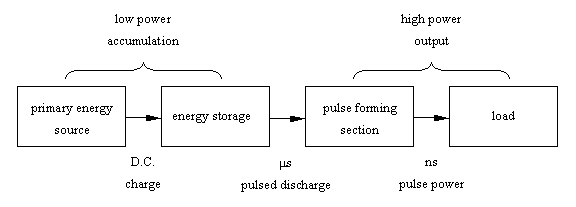
\includegraphics[height=4cm,width=8cm,keepaspectratio=true]{HPMsystem}
 \caption{Primjer ubacivanja slike.}
 \label{fig:prva}
	\end{center}
\end{figure}
\end{verbatim}
Uo�ite uporabu naredbe \verb|\label| unutar bloka. Na nju se potom u tekstu mo�emo referencirati pisanjem npr.\ \verb|Na Slici~\ref{fig:prva}| �ime \LaTeX{} u tekst uvrsti pripadaju�i broj slike, kao npr.\ ``Na Slici~\ref{fig:prva} prikazana je osnovna shema HPM sustava.''
Znak \verb|~| iza rije�i Slici osigurava to�no jedan znak razmaka, �to poma�e ukoliko je rije� Slika na kraju retka, da ne razdvoji rije� Slika i pripadaju�i broj slike.

\begin{figure}[!htbp]
	\begin{center}
 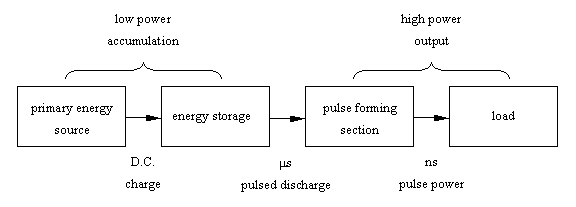
\includegraphics[height=4cm,width=8cm,keepaspectratio=true]{HPMsystem}
 \caption{Primjer ubacivanja slike.}
 \label{fig:prva}
	\end{center}
\end{figure}

Uo�ite i na�in prilago�avanja veli�ine slike. Parametri slike \emph{width} i \emph{height} odre�uju maksimalne dopu�tene dimenzije pri �emu se primarno po�tuje manju navedenu dimenziju, a \emph{keepaspectratio} osigurava zadr�avanje odnosa dimenzija slike, odnosno sprje�ava deformaciju slike, nakon proizvoljno unesenih veli�ina.

Uo�ite da sve oznake tj.\ \emph{labeli} ne smiju imati razmak u imenu. To vrijedi i op�enito, a ne samo za slike.

Tako�er, uo�ite da nije potrebno pisati ekstenziju slike jer to je ure�eno u postavkama glavnoga dokumenta pa time �tedi trud. Ekstenzije koje se mo�e izostaviti su: \emph{jpg}, \emph{jpeg}, \emph{png} i \emph{pdf}.

Shema prikazana na Slici~\ref{fig:prva} �e biti kori�tena i za potrebe idu�ih primjera, a {\color{blue} u mapi na va�em disku ju obri�ite nakon �to po�nete pohranjivati vlastite slike vezane uz va� rad}.


\section{Ubacivanje podslika}
Ponekada se jedna slika sastoji od dvije ili vi�e podslika kojima �elimo opisati neku cjelinu. Slika �e dobiti pripadni broj, a podslike slova (a), (b) itd.
To se mo�e posti�i sljede�om strukturom:
\begin{verbatim}
\begin{figure}[!htpb]
 \begin{center}
  \subfloat[Blok shema HPM sustava.]{\label{fig:HPM}
   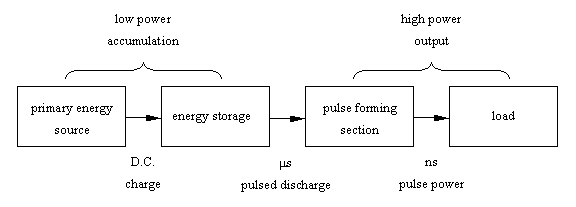
\includegraphics[height=5cm,width=10cm,keepaspectratio=true]{HPMsystem}}\\ 
	    %\hspace{10pt}
   \subfloat[JabRef su�elje za unos ``elektroni�ke'' reference.]
   {\label{fig:jabref}
   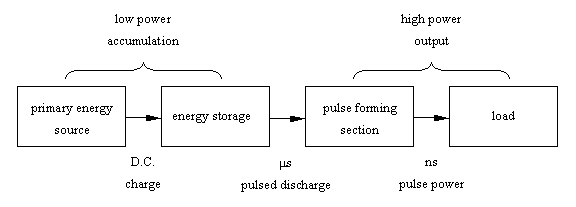
\includegraphics[height=7cm,keepaspectratio=true]{HPMsystem}}
\caption{Primjer ubacivanja vi�e podslika. Ovo je opis cijele slike.}
\label{fig:dvije_podslike}
  \end{center}
\end{figure}
\end{verbatim}
�to �e uvrstiti ono �to se vidi na Slici~\ref{fig:dvije_podslike}, koja se sastoji od dviju podslika.
Podslika~\ref{fig:HPM} pokazuje shemu HPM sustava, a podslika~\ref{fig:jabref} su�elje JabRef programa za unos bibliografskih jedinica.

\begin{figure}[!htpb]
	  \begin{center}
	   \subfloat[Blok shema HPM sustava.]{\label{fig:HPM} 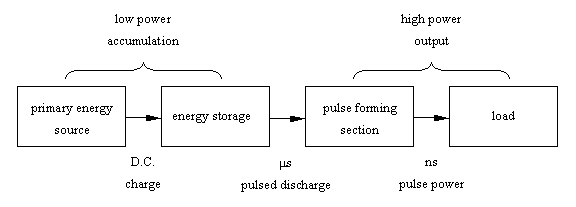
\includegraphics[height=5cm,width=10cm,keepaspectratio=true]{HPMsystem}} \\ %\hspace{10pt}
	   \subfloat[JabRef su�elje za unos ``elektroni�ke'' reference.]{\label{fig:jabref} 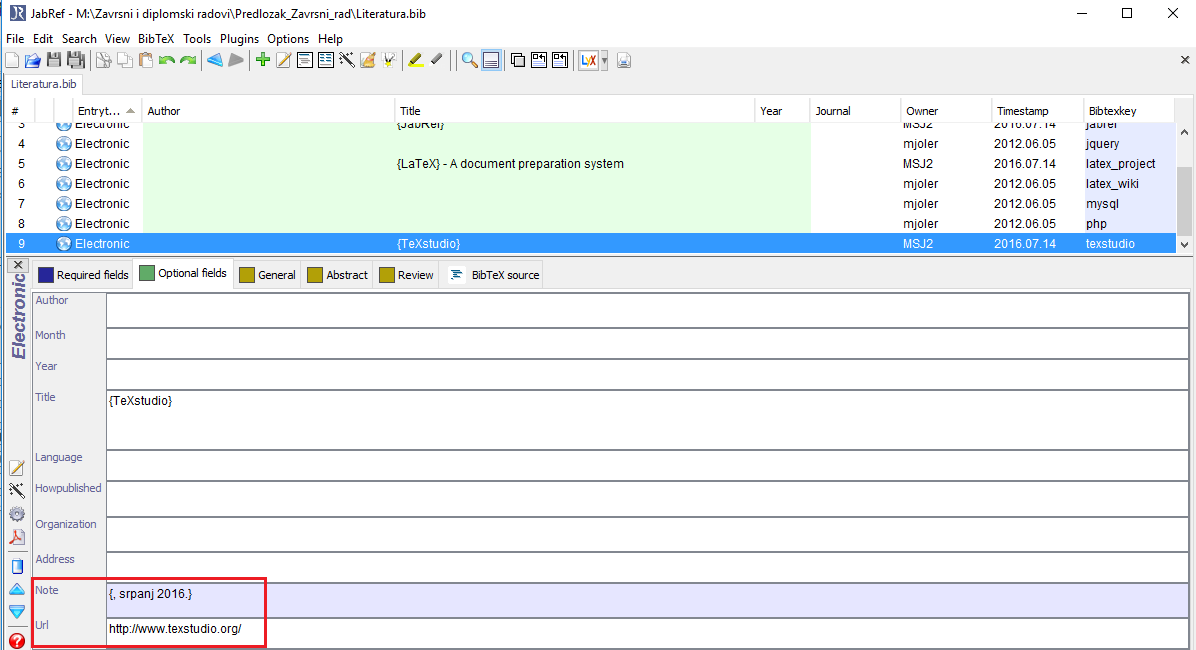
\includegraphics[height=7cm,keepaspectratio=true]{jabref}}
\caption{Primjer ubacivanja vi�e podslika. Ovo je opis cijele slike.}
\label{fig:dvije_podslike}
	  \end{center}
\end{figure}



\section{Ubacivanje tabele} 
Vi�e detalja o kreiranju tabela pro�itajte u literaturi, a sljede�i blok vam omogu�ava kreiranje jednostavne tabele, kao �to je prikazano u Tabeli~\ref{tab:prva}.
\begin{verbatim}
\begin{table}[!htbp]
\renewcommand{\arraystretch}{1.2}
\caption{Ovo je primjer izrade tabele.}
\centering
\begin{tabular}{|c|c|c|}
\hline
variabla & vrijednost 1 & vrijednost 2  \\ [0.5ex]
\hline \hline  
A & 5 & 3 \\ [0.5ex] % razmak do iducega retka
B & 4 & 2 \\ [0.5ex]
\hline
\end{tabular}
\label{tab:prva}
\end{table}
\end{verbatim}

\begin{table}[!htbp]
\renewcommand{\arraystretch}{1.2}
\caption{Ovo je primjer izrade tabele.}
\centering
\begin{tabular}{|c|c|c|}
\hline
variabla & vrijednost 1 & vrijednost 2  \\ [0.5ex]
\hline \hline 
A & 5 & 3 \\ [0.5ex] % razmak do iducega retka
B & 4 & 2 \\ [0.5ex]
\hline
\end{tabular}
\label{tab:prva}
\end{table}
%
Podaci koji su u stupcima se u tabeli razdvajaju znakom \&. Novi redak se na kraju aktualnoga retka formira znakom \verb|\\|. Broj stupaca se definira iza \emph{tabular} time �to se navedu slova koja ozna�avaju poravnavanje teksta u svakom stupcu, a broj slova zna�i broj stupaca koji �e biti kreiran u tabeli. Vertikalni razmak izme�u redaka u tabeli mo�ete za cijelu tabelu prilagoditi uporabom sljede�e sintakse prije strukture za tabelu:\\
\verb| \renewcommand{\arraystretch}{1.2} | gdje broj u zagradi na kraju (ovdje je 1.2) prilagodite sukladno va�oj preferenciji. Mo�e se prilagoditi i razmak za svaki pojedini redak (uo�ite \verb|[0.5ex]| na kraju redaka), ali to je manje od interesa jer tipi�no �elimo da svi retci imaju jednaki razmak jedni od drugih.

Sli�no mo�ete u�initi i za razmak izme�u stupaca tabele navo�enjem sljede�e sintakse prije bloka tabele:\\
\verb| \renewcommand{\tabcolsep}{0.3cm} |.



\section{Uporaba kratica u tekstu. Automatsko generiranje popisa kratica.}  \label{sec:kratice}
Listu kratica definirajte u datoteci \verb|Kratice.tex| (vidjeti predlo�ak unutar datoteke). U redovitom tekstu, kraticu  mo�ete ubaciti kori�tenjem naredbe \verb|\gls{ID_kratice}| gdje je \verb|ID_kraticE| identifikator kratice kako je definiran u datoteci \emph{Kratice.tex}. Pri prvoj uporabi naredbe \verb|\gls|, ispisat �e se najprije puni naziv pojma pa u zagradi kratica, a kod svake sljede�e uporabe, ispisat �e se samo kratica. Na primjer, kada (nakon prethodnog deklariranja u datoteci \verb|Kratice.tex|) upotrijebite \verb|\gls{gsm}| prvi puta, u tekstu �e se ispisati \gls{gsm}, a kada upotrijebite \verb|\gls{gsm}| drugi puta i dalje, u tekstu �e se ispisati samo \gls{gsm} (usporedi s definicijom kratice u datoteci \verb|Kratice.tex|). 
 
{\color{red} Listu kratica generirate sljede�im postupkom:} \label{generiranje_liste_kratica}
\begin{enumerate}
	\item Pokrenite kompilaciju cijeloga teksta jedanputa (to �e generirati neke datoteke koje su potrebne za daljnju obradu, specifi�no one s ekstenzijama .ist i .glo).
	\item Otvorite \emph{Command Prompt} aplikaciju na va�em ra�unalu i postavite se u radnu mapu gdje su vam datoteke za diplomski rad. 
	\item Potom pokrenite \emph{makeindex} rutinu (ona �e tipi�no biti ve� prisutna na va�em ra�unalu) upisuju�i sljede�u sintaksu: \\
	\verb|makeindex   -s myDoc.ist  -o myDoc.gls   myDoc.glo| \\
	gdje naziv datoteke \emph{myDoc} treba zamijeniti nazivom va�e glavne .tex datoteke, (npr. \verb|JMBAG_Ime_Prezime.tex|).
	\item Pokrenite \LaTeX{} jo� jednom ili dva puta, ako treba, dok se u uvodu pdf dokumenta ne pojavi lista kratica (pod naslovom \emph{Pojmovnik}).	
\end{enumerate}

Mo�da isprva zvu�i slo�eno, ali zapravo nije (bar ne uz ovako precizne upute!). Svaki puta kada dodate nove definicije kratica, potrebno je ponoviti ovaj postupak da bi se a�urirale odgovaraju�e datoteke i uredno prikazala potpuna lista u pdf-u (a i izbjegle poruke o pogre�kama tijekom kompajliranja teksta). 

Nije te�ko nakon �to prvi puta pro�ete ovaj postupak i omogu�ava vam u tekstu biti dosljedan u uporabi odre�ene kratice. Da izbjegnete �u�enje, va�no je jo� re�i da �e se ovim postupkom automatski stvoriti tek lista kratica koje ste u tekstu upotrijebili uporabom sintakse \verb|\gls|, a ne na temelju liste definicija koje ste naveli u datoteci \verb|Kratice.tex|. Zato, ako nijednom u tekstu ne upotrijebite sintaksu \verb|\gls|, ne�e biti ispisan ni popis kratica tj.\ \emph{Pojmovnik}. {\color{blue} Kako \LaTeX{} na kraju uvijek nagradi trud koji je ulo�en u savladavanje njegove sintakse, pogodnost ovakvoga automatskoga kreiranja Pojmovnika je i to �to uz svaki kraticu \LaTeX{} automatski ispi�e i brojeve stranica na kojima se doti�na kratica pojavljuje!} U elektroni�kom pdf dokumentu, brojevi stranica su ujedno i hiper-veze na te stranice pa se tako mo�e odmah sko�iti na stranicu gdje je pojedina kratica upotrijebljena.

Ukoliko vam se prethodno opisani postupak �ini preslo�enim, popis kratica mo�ete napraviti i ru�no, isto pomo�u datoteke Kratice.tex, u kojoj tako�er postoji kratki predlo�ak i za takav pristup. Za to je onda u osnovnoj datoteci \verb|JMBAG_Ima_Prezime.tex| potrebno deaktivirati liniju koda koja po�inje sa \verb|\printglossary|, a aktivirati blok koji po�inje sa \verb|\begin{glossary}| i zavr�ava sa \verb|end{glossary}|.



\section{Nagla�avanje teksta}
\subsection{Navodnici}
Za navodnike s lijeve strane fraze (otvaranje navodnika) koristi se 2x jednostruki navodnik koji se na tipkovnici nalazi lijevo od broja 1, a za navodnike s desne strane fraze (zatvaranje navodnika), koristi se 2x jednostruki navodnik koji se na tipkovnici nalazi na tipki \emph{�}, �to proizvede npr.\ ``abc''.

{\color{blue} Alternativno, u ovom paketu je pripremljena i naredba {\color{red} \verb|\navod{abc}|} gdje je \emph{abc} tekst koji se stavlja izme�u navodnika, tj.\ \navod{abc}.}

\subsection{Kosa i podebljana slova}
Nagla�avanje neke rije�i ili fraze pomo�u kosih (italic) slova mo�emo dobiti uporabom naredbe {\color{red} \verb|\emph{abc}|} ili pomo�u  {\color{red}\verb|\textit{abc}|} gdje je \emph{abc} neki tekst koji se �eli naglasiti.

\textbf{Podebljana slova} mo�emo posti�i uporabom naredbe {\color{red} \verb|\textbf{abc}|} gdje je \textit{abc} neki tekst koji �elimo podebljati.

\section{Verbatim: okru�enje za doslovni tekst}
Verbatim okru�enje omogu�ava ispis teksta u izvornom obliku, bez da ga \LaTeX{} tuma�i po svojiim sintakti�kim pravilima. To je pogodno kada se na stranicu  npr.\ �eli kopirati dio programskoga koda iz nekog jezika i kada �elimo zadr�ati sve izvorne znakove u nekoj frazi, bez da \LaTeX{} po�ne javljati pogre�ke kod kompajliranja, �to bi se moglo pojaviti kada se ne bi koristilo \emph{verbatim okru�enje}, po�to bi neke znakove interpretirao kao pogre�ke u sintaksi.

Postoji kra�i i du�i oblik verbatima. Kra�i slu�i za kra�u frazu od jedne ili par rije�i, a du�i za vi�e redaka.

\noindent Kra�i oblik verbatima ima sintaksu: \verb+\verb|neka fraza|+

\noindent Du�i oblik verbatima ima sintaksu:\\
\verb|\begin{verbatim}| \\
\verb|neki tekst| \\
\verb|\end{verbatim}| \\


\section{Kreiranje jedne jednad�be ili serije jednad�ba}

\subsection{Kreiranje jedne jednad�be}
Jednad�ba se napi�e u posebnom matemati�kom modu koji se kreira pomo�u bloka:
\begin{verbatim}
	\begin{equation}
		 A = B + C   \label{eq:prva}
	\end{equation}
\end{verbatim}
�to �e dati sljede�i izgled:
\begin{equation}
	 A = B + C   \label{eq:prva}
\end{equation}
Da bi se na nju referenciralo, na �eljenom mjestu u tekstu upi�emo \verb|\eqref{eq:prva}|, �ime �e se uvrstiti njezin pripadni (automatski generirani) broj, a za potpuniji smisao mo�emo npr.\ napisati \verb| Jednad�ba~\eqref{eq:prva}|, rezultat �ega je da �e u tekstu pisati Jednad�ba~\eqref{eq:prva}. 
Ako ju se ne �eli numerirati, onda se nakon rije�i \emph{begin} stavi zvjezdica, tj.\ \verb|begin*{equation}|.

\subsection{Kreiranje grupe jednad�ba}
Grupa jednad�ba se kreira uporabom \emph{subequations} sintakse. Na primjer, sljede�i blok �e definirati dvije podjednad�be u grupi, gdje �e svaka biti numerirana istim brojem, a razlikovati slovom iza broja.
\begin{verbatim}
	\begin{subequations}
		\begin{align}
		        A &= B + C  	\label{subeq:prva} \\
		        D &= F + G		\label{subeq:druga}
		\end{align}
	\label{subeq:obje}
	\end{subequations}
\end{verbatim}

To �e u izlaznom dokumentu rezultirati sljede�im izgledom:
\begin{subequations}
\begin{align}
        A &= B + C  	\label{subeq:prva} \\
        D &= F + G		\label{subeq:druga}
\end{align}
\label{subeq:obje}
\end{subequations}
U \eqref{subeq:prva} je prikazano dobivanje vrijednosti $A$, a u \eqref{subeq:druga} je prikazano dobivanje vrijednosti $D$. Jednad�ba~\eqref{subeq:obje} je \emph{�uveni studentov zakon}!



\section{Liste}
Liste su �este forme u tekstu kojima se na pregledni na�in nabrajaju neke stavke. Stavke obi�no navodimo ili s to�kama na po�etku, s brojevima ili sa slovima. U \LaTeX-u su upravo ta tri stila unaprijed definirana, a mogu�e su i slo�enije definicije stilova i kombinacije lista.

\subsection{Lista s to�kama}
Lista s to�kama se postigne blokom
\begin{verbatim}
\begin{itemize}
    \item prva nenumerirana stavka
    \item druga nenumerirana stavka
\end{itemize}
\end{verbatim}
�to na ekranu proizvede:
\begin{itemize}
% \setlength\itemsep{1ex}   % za lokalnu prilagodbu
	\item prva nenumerirana stavka
	\item druga nenumerirana stavka
\end{itemize}

\subsection{Lista s brojevima}
Numerirana lista s brojevima se postigne blokom
\begin{verbatim}
\begin{enumerate}[itemsep=1ex, topsep=4pt, partopsep=0pt]
     \item prva numerirana stavka
     \item druga numerirana stavka
\end{enumerate}
\end{verbatim}
U uglatoj zagradi su tri parametra kojima se to�no mo�e kontrolirati vertikalni razmak izme�u stavki u listi (\emph{itemsep}), razmak izme�u prethodnoga teksta i prve stavke u listi (\emph{topsep}) i dodatni prostor izme�u liste i prethodnoga paragrafa kada lista zapo�inje novi paragraf (\emph{partopsep}), ali te parametre \textbf{ne morate navoditi} tj.\ tu uglatu zagradu ne morate pisati. Tada �e se primijeniti vrijednosti parametara koje su definirane za cijeli dokument, a ove parametre se mo�e upotrijebiti tek da u nekom pojedinom slu�aju prilagodite razmake.
Za osjetiti efekte ovih parametara, najbolje se malo sam poigrati razli�itim vrijednostima parametara i vidjeti posljedice toga na listu (pri tome se uz brojeve kao prikladne jedinice za razmak mogu koristiti \emph{pt}, \emph{ex} ili \emph{em}).

\subsection{Proizvoljno ozna�ena lista}
Takva se lista mo�e posti�i u sklopu op�enitije forme koja omogu�uje proizvoljni opis ispred pojedine stavke, pomo�u sljede�ega bloka:
\begin{verbatim}
\begin{description}
     \item[a)] prva opisna stavka
     \item[b)] druga opisna stavka
\end{description}
\end{verbatim}
�to na ekranu proizvede:
\begin{description}%[itemsep=1ex, topsep=4pt, partopsep=0pt] za lokalnu prilagodbu
	\item[a)] prva opisna stavka
	\item[b)] druga opisna stavka \\
\end{description}
%
Kod ove strukture, u uglatu zagradu iza naredbe \verb|\item|, navodi se proizvoljna oznaka kojom se �eli na neki na�in ``numerirati'' listu.
%:::::::::::::::::::::::::::::::::::::::::::::::::::
\chapter{Dodatne informacije}
\section{Primjeri uporabe sintakti�kih struktura}
\begin{enumerate}
	\item Za uvid u kontekstualnu primjenu raznih sintakti�kih struktura, mo�ete otvoriti datoteku \href{run:Intro.tex}{{\color{blue}Intro.tex}}, unutar koje su napisane i ove upute. 
	\item Primjere slo�enijih sintakti�kih struktura, kao �to su ubacivanje slike, tabele ili jednad�be, mo�ete na�i u datoteci \href{run:sintaksa_cestih_struktura.tex}{{\color{blue}sintaksa\_cestih\_struktura.tex}} koja je dio paketa. Odabrane se strukture mo�e kopirati i zalijepiti u va� tekst, uz minimalne prilagodbe kao �to su naziv slike, veli�ina slike, opis i ID slike, a analogno i za tabele i jednad�be.
	\item Kona�no, za vi�e detalja o bilo �emu, potra�ite informacije u dvama priru�nicima koji su prilo�eni u mapi \href{run:prirucnici}{{\color{blue}prirucnici}} ili na webu, gdje se, me�u obiljem drugih informacija, nalaze i korisne wiki stranice \cite{latex_wiki,tex_exchange} o \LaTeX-u pomo�u kojih se obi�no brzo prona�e upute i zadovoljavaju�e rje�enje kakvom sintaksom se mo�e urediti �eljeni dio teksta.
\end{enumerate}

\section{Savjeti za lak�e ure�ivanje teksta}
Vjerujem da vam ovaj dokument mo�e uvelike pomo�i u pripremi teksta va�ega zavr�nog/diplomskog rada i omogu�iti da glavninu vremena tro�ite na sadr�aj rada, a manje na formatiranje rada jer to �e za vas sada obaviti \LaTeX{}! 

No, korektnosti radi, potrebno je napomenuti i sljede�e: \LaTeX{} je vrlo osjetljiv na pogre�ke u sintaksi naredbi (da, ba� kao �to su i programski jezici) pa vas mo�e povremeno ugnjaviti javljanjem pogre�ke koju nikako ne uspijevate uo�iti gdje je. Iskustvo kojim se izbjegava ta nelagoda jest sljede�e:
\begin{itemize}
	\item svako poglavlje napi�ite u novoj datoteci (da biste koli�inu teksta razdvojili na preglednije i manje cjeline) koju imenujte prikladnim imenom (bez razmaka u imenu). Potom te datoteke samo pozivajte iz glavnoga dokumenta \verb|JMBAG_Ime_Prezime.tex| pomo�u naredbe \verb|\include{ime_datoteke}|. Takav je pristup upravo i kori�ten u pripremi ovoga paketa.
	%
	\item {\color{red} budite koncentrirani dok pi�ete \LaTeX{} naredbe, poglavito zagrade, posebne znakove i matemati�ki tekst gdje se zahtijeva uporaba znaka \$!}
	%
	\item kompajlirajte tekst prije nego se skupi puno teksta jer tako �ete imati manje teksta za prekontrolirati u slu�aju pogre�ke. Tako�er vam za provjeru tek manjega dijela dokumenta mo�e pomo�i paket \verb|\usepackage{syntonly}| i naredba \verb|syntaxonly|, a isto tako i naredba \verb|\includeonly{ime_datoteke}| kojom �ete kompajlirati samo tu navedenu datoteku, �ime  ispred ``ne�eljenih'' datoteka ne morate stavljati znak ``komentara'' (\%).
	%
	\item ako niste sigurni ho�e li vam raditi neka naredba nakon pisanja, radije tekst kompajlirajte odmah po pisanju te naredbe---da vidite �to �ete dobiti i rije�ite dvojbu, nego da �ekate da se skupi jo� dubioznih mjesta u tekstu, kada �e nakon kompajliranja biti te�e detektirati koja linija teksta zapravo izaziva probleme (\LaTeX-ov prozor s porukama �esto nije odve� precizan u lociranju i opisu pogre�aka, ovisno o editoru teksta koji koristite).
\end{itemize}


\section{Zavr�ne napomene}
Ovime zaklju�ujemo uvodne upute koje �e najve�em broju studenata biti dovoljne (ili barem dovoljna osnova) za uspje�no pisanje zavr�nog odnosno diplomskog rada.

Prije nego prije�ete na kreiranje vlastitoga sadr�aja u�inite jo� sljede�e akcije kojima �ete deaktivirati dio paketa koji �e biti nepotreban:
\begin{enumerate}
	\item u mapi \href{run:slike}{{\color{blue}slike}}, obri�ite datoteke \verb|HPMsystem.png| i \verb|jabref.png| jer su one slu�ile tek za ilustracije u ovim Uputama.
	%
	\item u glavnoj datoteci  \href{run:JMBAG\_Ime\_Prezime.tex}{{\color{blue}JMBAG\_Ime\_Prezime.tex}} stavite znak komentara ``\%'' ispred linije \verb|\chapter{Kako koristiti paket za pisanje zavr�noga rada u \LaTeX-u}
Ovo su uvodne napomene za kori�tenje predlo�ka za pisanje zavr�noga ili diplomskoga rada studenata Tehni�koga fakulteta u Rijeci. Prije kori�tenja paketa, pro�itajte ovaj tekst jer �e vam dati nu�ne uvodne informacije, znatno vam olak�ati i ubrzati ure�ivanje teksta nakon toga, pri �emu �e vas i voditi kroz uporabu ovoga paketa na prakti�an na�in.

Paket je pripremljen tako da student �to prije mo�e pisati vlastiti tekst u ve� pripremljenom predlo�ku koji �e, uz minimalno u�enje sintakse \LaTeX-a, studentu olak�ati urediti svoj rad. U paketu su uklju�ene potrebne upute i sintakti�ke strukture koje bi trebale udovoljiti potrebama ve�ine studenta, a dodatne informacije postoje u dvama priru�nicima koji su uklju�eni u ovom paketu te, naravno, na raznim web stranicama na internetu koje su posve�ene \LaTeX-u (vidi u nastavku).

{\color{red} POZOR: paket treba biti prekopiran negdje na disk ne mijenjaju�i originalnu strukturu mapa (foldera) i ne mijenjaju�i nazive datoteka koje su u mapi \emph{tex\_aux}!}


\section{Opis sadr�aja paketa}
\vspace{-2ex}
Paket se sastoji od:
\begin{itemize}
 \item datoteke \href{run:UPUTE.pdf}{{\color{blue} UPUTE.pdf}} koja sadr�i postupak instalacije potrebnih alata na ra�unalo te kori�tenja paketa. \emph{UPUTE} su bazirane na Windows OS, a korisnici drugih OS-ova si na nazna�enim web lokacijama samo trebaju na�i instalacije za njihov OS.
 %
 \item datoteke \verb|JMBAG_Ime_Prezime.tex| koja je sredi�nja datoteka koja povezuje sve cjeline i kompajliranjem koje se dobije izlazni \verb|JMBAG_Ime_Prezime.pdf| dokument (naravno, tijekom rada, upisat �ete svoj specifi�ni JMBAG i ime i prezime).\\ U ovoj se datoteci inicijalno nalaze i upute za kori�tenje paketa kao i primjeri osnovne uporabe naj�e��ih sintakti�kih struktura u \LaTeX-u koje bi trebale biti dovoljne ve�ini studenata za pisanje rada.
 %
 \item mape \verb|tex_aux| u kojoj su \emph{interne datoteke} koje definiraju stilove, formate i sl.\ koji slu�e u slaganju izlaznoga formata. \textbf{Student/ica s njima ne treba \emph{ni�ta} raditi}, ali one trebaju biti u \verb|tex_aux| mapi pod glavnom mapom zavr�noga rada, kao �to je postavljeno u ovom paketu.
 %
 \item mape \emph{slike} u koju student treba pohraniti sve slike koje �e koristiti u radu. Ime mape se ne smije preimenovati bez boljega poznavanja sintakse \LaTeX-a jer ovaj paket da bi ispravno radio o�ekuje ba� takvo ime mape!
 %
 \item datoteke \verb|sintaksa_cestih_struktura.tex| koja ne sudjeluje izravno u kompajliranju pdf dokumenta, nego slu�i kao repozitorij u kojemu su sadr�ane naj�e��e potrebne sintakti�ke strukture koje su spremne za kopiranje u va� tekst uz minimalnu prilagodbu parametara (npr.\ opis slike, ime datoteke specifi�ne slike koju se ubacuje i proizvoljni ID te slike za kasnije referenciranje).
 %
 \item mape \href{run:prirucnici}{{\color{blue}prirucnici}} u kojoj se nalazi nekoliko najpopularnijih priru�nika za uporabu \LaTeX-a. 
\end{itemize}
%%%%%%%%%%%%%%%%%%%%%%%%%%%%%%%%%%%%%%%%%%%%%%%%%%%%%%%%%%%%%%%

\section{�ime se opremiti za pisanje rada}
Da bi se rad napisao pomo�u \LaTeX-a (a to vrijedi svake lipe!), najprije je na ra�unalo potrebno instalirati:
\begin{enumerate}
	\item obavezno: \LaTeX{} software 
	\item obavezno: editor za ure�ivanje teksta 
	\item neobavezno, ali korisno: softver za opis literature. (Premda dodatni softver nije nu�an jer se popis literature mo�e obraditi i ru�no (no to je manje sofisticirano kod uvr�tavanja referenca), sugeriram instalaciju softvera koji pomo�u intuitivnih su�elja korisniku omogu�ava opis pojedine kori�tene literature (kao mala baza podataka), a potom se pojedina jedinica literature jednostavno ubacuje u tekst, a popis literature se na kraju automatski formira (vi�e o tome pro�itajte u nastavku).
\end{enumerate}

\subsection{Instalacija \LaTeX-a}
\begin{enumerate}
	\item odite na sredi�nji \LaTeX{} portal \cite{latex_project}: \url{http://www.latex-project.org/}
	\item kliknite na poveznicu \href{http://www.latex-project.org/ftp.html}{Getting LaTeX} i potom uo�ite i povucite instalaciju koja odgovara va�em OS-u (npr.\ proTeXt za Windows, MacTeX za Mac, TeX Live za Linux). Pozor: instalacijski paket je velik i mo�e du�e potrajati �ak i na brzoj vezi---dajte si dovoljno vremena za obaviti download.
	\item Instalirajte \LaTeX{} slijede�i upute koje su prilo�ene za odabranu instalaciju (npr.\ proTeXt za Windowse daje kratki pdf s uputama koje vas vode kroz instalaciju korak po korak).
\end{enumerate}

\subsection{Instalacija editora teksta}
Instalirajte editor koji je pogodan za pisanje \LaTeX{} koda. \textbf{Za Windows OS, toplo preporu�am}  \href{http://www.texstudio.org}{{\color{blue} TeXstudio}} \cite{texstudio} jer je bogat opcijama, ugodan za rad i stabilan, a instalacije postoje i za Linux i Mac OS. TeXstudio se zasebno povu�e i instalira na ra�unalo, a neke editore teksta koji ve� do�u u paketu za instalaciju LaTeXa mo�ete ignorirati (npr.\ za Windows je do nedavno bio popularan \emph{TeXnicCenter} i dolazi ve� upakiran u proTeXt-u (a mo�da �ete na�i i \emph{TeXworks}), za Mac je kvalitetan \emph{TeXShop} koji sada tako�er dolazi u paketu s MacTeX-om). 

\label{encoding1} {\color{red} POZOR: Premda �e ovo biti jo� napomenuto na stranici~\pageref{encoding2}, prije samoga po�etka pisanja va�ega rada, �to prije �elim napomenuti sljede�i va�ni detalj: za svaki va� tekst koji pi�ete u editoru teksta, uvjerite se da je kodna stranica postavljena na \navod{windows-1250}, �to je klju�no da bi se u izlaznom pdf-u ispravno ispisivali hrvatski dijakriti�ki znakovi! U TeXstudiu, aktualnu kodnu stranicu se mo�e vidjeti i promijeniti preko maloga izbornika u doljnjem desnom kutu glavnoga prozora, gdje se nalazi opcija ``Encoding''. Ukoliko tu ne pi�e ``windows-1250'', kliknite na izbornik, odaberite opciju ``More Encodings'' pa u potom otvorenom su�elju odaberite kodnu stranicu ``windows-1250 / CP 1250'' i potvrdu sa ``Change To''.}

\subsection{Instalacija programa za opis kori�tene literature}
\emph{Ponavljamo: Kori�tenje BiBTeX programa za opis literature \textbf{nije} neophodno, ali jest korisno. U datoteci po imenu \href{run:Literatura.tex}{{\color{blue}Literatura.tex}}, koja je uklju�ena u ovaj paket, ve� su namje�tene postavke kao da �e se literatura opisati pomo�u BiBTeX programa (npr.\ JabRef-a) i ne treba ni�ta mijenjati, ali ispod toga se mo�e prona�i i upute i za drugi--ru�ni-- na�in (p)opisivanja literature.}

Kao bibtex program za opis literature, preporu�am \href{http://www.jabref.org}{{\color{blue} JabRef}} program \cite{jabref}. To je legalno besplatno dostupni program za Windows OS (ali postoji i za Mac, a i platformski neovisna instalacija) koji nam omogu�ava opisivanje literature na lak na�in pomo�u intuitivnih su�elja, a kao rezultat kreira \emph{BibTeX} datoteku \emph{Literatura.bib} (gdje je (\emph{Literatura} naziv koji korisnik treba dodijeliti pri pohrani JabRef datoteke na disk u slu�aju ovoga predlo�ka, da bi paket funkcionirao) u kojoj je literatura opisana na na�in koji \LaTeX{} razumije. 

Uo�ite da ako ne koristite JabRef, ve� se odlu�ite za ru�ni unos literature, �to se isprva doima jednostavnijim, tada �e vam redoslijed referenca u popisu literature odgovarati to�no redoslijedu koji ste naveli u tom popisu --- dakle morate paziti da redoslijed formirate onim redom kojim pozivate reference u va�em tekstu (�to kod nekog kasnije ubacivanja dodatne reference unutar ve� postoje�ega redoslijeda tra�i brigu da ju se ubaci na odgovaraju�e mjesto u popisu literature), a tako�er trebate paziti i na formatiranje teksta svake reference! 

Za razliku od toga, kori�tenjem JabRef-a, izbjegavate ru�no formiranje popisa literature i ne trebate brinuti o redoslijedu referenca, ve� samo pomo�u JabRefa trebate unijeti sve jedinice literature koju �ete navesti, a \LaTeX{} �e vam automatski formirati listu referenca onim redoslijedom kojim reference bude pozivali u tekstu!

Nakon �to kompajlirate projekt, stvorit �e vam se pomo�na datoteka imena \href{run:JMBAG_Ime_Prezime.bbl}{{\color{blue}JMBAG\_Ime\_Prezime.bbl}} u kojoj �e jedinice literature tijekom kompilacije biti formatirane i odatle se ubacuju u kona�nu verziju teksta. Stoga, \textbf{ukoliko ima ikakvih detalja koje u opisu literature treba prilagoditi, a ne mo�ete automatskim putem}, uvijek vam kao ``zadnja crta obrane'' ostaje otvoriti \verb|bbl| datoteku i tamo ru�no napraviti izmjene. Potom ponovo kompajlirajte projekt i te �e se promjene vidjeti u pdf-u tj.\ ru�no unijete promjene ne�e biti poni�tene sve dok ne obri�ete cijelu datoteku.

Umjesto da rukom pi�ete cijelu bibliografiju, vremenski vam je vjerojatno u�inko\-vitije popis literature generirate uporabom JabRef-a, a potom ako i�ta jo� treba prilagoditi, onda samo to napraviti ru�no u \verb|bbl| datoteci.


\subsubsection{Osnovna uporaba JabRef programa}
Upoznajte se s najva�nijim opcijama u \emph{JabRef}-u:
\begin{itemize}
	\item uo�ite ikonu (pod znakom ``+'' i tekstom \emph{New BibTeX Entry}) za unos nove jedinice literature (npr. knjige, �lanka, web portala i sl.)
	%
	\item kada kliknete za unos nove stavke literature, uo�ite kakvi se sve tipovi literature nude za odabir. Odabirom opcije koja odgovara naslovu koji �elite unijeti, otvorit �e vam se novi prozor s poljima u koja se mo�e unijeti informacije o literaturi. Za odabrani tip literature samo su neka polja obavezna (nalaze se pod karticom (eng.\ \emph{tabom}) \emph{Required fields}), dok se pod drugim karticama mo�e i ne mora unijeti dodatne informacije. U slu�aju na�ih zavr�nih/diplomskih radova, bit �e znatan udjeli literature koja je na internetu pa za formatiranje iste, pro�itajte upute i napomene u nastavku ove sekcije.
	%
	\item kada je vi�e autora, njihova imena se u JabRefu polju za unos autora razdvajaju pisanjem klju�ne rije�i \verb|and| (a ne razmakom, zarezom ili to�ka-zarezom!)
	%
	\item U popisu literature se ne�e uvijek pojam prepisati onako kako ste ga vi zapisali u JabRefu! To je posljedica stilova koji su definirani u \verb|bst| datoteci (ne zamarajte se time sada jer je za naprednu razinu \LaTeX-a). No, ako neki pojam ba� ne ispadne suvislo napisan u popisu literature ili ba� �elite forsirati odre�eni na�in zapisa (�esto slu�aj kada se rije� s velikim slovima ne interpretira onako kako �elite), tada to�no odre�eni zapis mo�ete forsirati na na�in da \verb|{tu rije� ili frazu stavite unutar viti�astih zagrada}|
	%
	\item prije nego pohranite pojedinu stavku pomo�u \emph{Ctrl+S}, \textbf{morate svakoj jedinici literature dodijeliti jedinstveni identifikator}, tzv.\ \emph{Bibtexkey}, �to je jedno od polja koja su obavezna za unos. Mo�ete ru�no upisati neki proizvoljni string, ali pogodnije je generirati ga automatski.\\ Za to u�initi me�u ikonama na vrhu imate ikonu koja izgleda kao (�arobni) �tapi� sa zvjezdicama oko njega, klikom na kojega \emph{JabRef} automatski dodijeli jedinstveni BibTeX \emph{klju�} za tu bibliografsku jedinicu. Pomo�u toga klju�a se poslije bilo kada i bilo gdje u pisanju va�ega rada mo�ete pozvati na tu referencu, a \LaTeX{} �e sve ostalo obaviti za vas tj.\ dodijeliti joj odgovaraju�i broj u tekstu i s tim brojem uvrstiti u popis literature.
	%
	\item korisnik ima mogu�nost i promijeniti uzorak po kojem se kreira struktura automatski generiranoga jedinstvenoga BibTeX klju�a tako da se otvori opcija izbornika \emph{Options $>>$ Preferences $>>$ BibTeX key generator}, gdje je na vrhu prozora prikazan \emph{default} uzorak, npr. \verb|[auth]:[year]| �to zna�i da se klju� kreira na bazi \verb|prezime(autora):godina(rada)|. To se sada mo�e urediti po nekom novom uzorku, no ovako definirani uzorak u biti zadovoljava, a ako igdje ima potrebe za dodatnim razlikovanjem, mo�e se na automatski generiranom klju�u jo� ru�no napraviti korekcija dodavanjem nekog znaka na kraju, kao npr.\ dodavanjem \verb|_a| i sl. (Klikom na karticu \emph{BibTeX source} mo�ete vidjeti kako �e unos va�ih podataka zapravo biti zapisan u va�oj \emph{Literatura.bib} datoteci koja �e se formirati od svih bibliografskih jedinica koje unesete.)
	%
	%
	\item Za \emph{ime} va�e bibliografske datoteke kod pohrane na disk obavezno upi�ite  \emph{Literatura} jer to ime o�ekuje ovaj paket. Pozor: Datoteka \emph{Literatura.bib}, koju ste tako kreirali, mora se nalaziti unutar mape ovoga paketa da bi sve ispravno radilo! U paketu je za primjer ve� kreirana jedna datoteka istoga imena koju za vje�bu student mo�e i otvoriti u \emph{JabRef}-u, ali to su samo pokazne bibliografske jedinice unesene kao primjer, koje student treba u kona�nici zamijeniti svojim bibliografskim jedinicama.
	%
	\item Za ``elektroni�ke'' izvore literature (tj.\ sve �to ste kao informaciju na�li na webu), JabRef nudi tip literature pod nazivom ``Electronic'' (vidi Sl.~\ref{fig:jabref}). U njemu pod karticom (eng.\ tabom) \emph{Optional fields} pod poljem \verb|Title| mo�ete upisati ime web stranice (autor, tvrtka i sl.), pod poljem \verb|url| mo�ete upisati URL adresu te web stranice, a pod poljem \verb|Note| upisati datum kada ste posjetili tu web stranicu (npr.\ \emph{srpanj 2016.} ili \emph{3.~rujna~2016.}). Rezultat toga �e u pdf-u biti da je sve napisano redoslijedom koji je predvi�en u Uputama RiTeha za pisanje diplomskog rada \cite{riteh_upute}, \emph{osim �to u ovom Predlo�ku do sada nisam uspio rije�iti ubacivanje zareza izme�u URL adrese i datuma posjeta toj URL adresi}, koji bi ta dva podatka odvojio, pa je tu potrebna mala ru�na \emph{prilagodba na jedan od ovih dvaju na�ina}:
	\begin{enumerate}[label=\textbf{\roman*)}]
		\item kod unosa datuma u polje \verb|Note| (u su�elju JabRef-a), upi�ite datum na sljede�i na�in: \verb|{, <datum>}|, gdje je \verb|<datum>| va� specifi�ni datum, dok �e \emph{zarez} iza prve zagrade izvr�iti razdvajanje URL adrese i datuma, a \textbf{viti�aste zagrade} osigurati da se to ba� tako to�no prenese u pdf-dokument (uklju�uju�i i da se mjesec napi�e malim po�etnim slovom, �to ina�e ne bi bio slu�aj). (Za neke druge tipove referenca kao npr.\ tip \emph{manual}, zarez vam prije datuma ne�e trebati jer �e naziv literature zavr�iti zarezom.) U Jabrefu vam i ina�e vrijedi da kada �elite forsirati da se pojam ba� to�no u popisu literature zapi�e onako kao ste htjeli, onda se pojam stavi unutar viti�astih zagrada \verb|{kao u ovom primjeru}|.
		\item ako u polju \verb|Note| ne upi�ete datum na prethodno opisani na�in, onda vam u pdf dokumentu ne�e biti upisan zarez izme�u URL adrese i datuma koji ste unijeli, a tako�er �e i mjesec biti napisan velikim po�etnim slovom (�to nije stra�no, ali je manje po�eljno). To mo�ete \emph{ru�no} prilagoditi tako da otvorite \verb|.bbl| datoteku i pomo�u \emph{Find/Replace} operacije sve nazive mjeseca zamijenite na na�in da po�inju malim po�etnim slovom (�to nije te�ko kada vam je ve�ina datuma u popisu literature navedena u istom mjesecu), ali zareze �ete svakako morati ubacivati ru�no u svaku pojedinu stavku literature jer ne�e biti nekog predlo�ka kojim biste to rije�ili automatski pomo�u \emph{Find/Replace} operacije. Na kraju opet kompajlirajte projekt. S obzirom na navedeno, prvi na�in je vremenski �tedljiviji!
	\end{enumerate}
\end{itemize}

%%%%%%%%%%%%%%%%%%%%%%%%%%%%%%%%%%%%%%%%%%%%%%%%%%%


\chapter{Primjeri naj�e��ih sintakti�kih struktura}
Prije stvarnoga po�etka pisanja svoga rada, upoznajte se s osnovnim sintakti�kim strukturama koje �e vam trebati tijekom pisanja rada.

U nastavku su opisane naj�e��e sintakti�ke strukture (dio njih mo�ete na�i i u datoteci \emph{Intro.tex}), a dodatne slo�enije strukture su pohranjene u datoteci \href{run:sintaksa_cestih_struktura.tex}{{\color{blue}sintaksa\_cestih\_struktura.tex}} koja je sastavni dio glave mape ovoga paketa. 

\section{Postavljanje naslova poglavlja i sekcija}
\begin{itemize}
	\item \verb|\chapter{Naslov poglavlja}|: za definiranje naslova poglavlja
	\item \verb|\section{Naslov sekcije}|: za definiranje naslova sekcije unutar poglavlja
	\item \verb|\subsection{Naslov podsekcije}|: za definiranje naslova podsekcije
\end{itemize}


\section{Reference na literaturu} \label{sec:RefLit}
Za referencu na pojedini kori�teni izvor informacije (tj.\ jedinicu literature), koristimo naredbu \\
\verb|\cite{bibtexkey}|, gdje je \emph{bibtexkey} jedinstveni klju� kojim prethodno ozna�imo tu jedinicu literature. \verb|Bibtexkey| mo�emo definirati na jedan od sljede�ih na�ina:
\begin{description}
	\item[I)] ako popis literature definiramo izravno u datoteci \href{run:Literatura.tex}{{\color{blue}Literatura.tex}} (opcija (I) u datoteci), onda ispred svake stavke literature treba definirati i jedinstveni \verb|bibtexkey| pomo�u naredbe \verb|\bibitem{bibtexkey}| (vidi predlo�ak u datoteci)
	\item[II)] ako literaturu opisujemo pomo�u JabRef datoteke \emph{Literatura.bib} (opcija (II) u datoteci), onda se tamo uz svaku stavku definira \verb|bibtexkey| (bude na dnu JabRef obrasca za upis pojedine jedinice literature)
\end{description}
%
Npr.\ ako negdje u tekstu napi�emo \verb|\cite{latex_wiki}|, gdje je \verb|latex_wiki| prethodno definirani \emph{bibtexkey}, tada �e se u tekstu u uglatoj zagradi pokazati broj  te bibliografske jedinice pod kojim se nalazi u popisu literature (Bibliografiji) na kraju rada (u ovom primjeru, to je broj \cite{latex_wiki}).


\section{Referenca na sekciju, sliku, tabelu ili stranicu} \label{sec:RefText}

Za referenciranje na pojedine dijelove teksta unutar rada, koristimo
{\color{red} \verb|\label{ID}|} i {\color{red} \verb|\ref{ID}|} na na�in da se \verb|\label{ID}| postavi uz dio teksta koji �elimo ozna�iti internom oznakom i poslije �emo se u tekstu na to referencirati, a \verb|\ref{ID}| upotrijebimo na mjestu s kojega se referenciramo na dio teksta koji je ranije ozna�en pomo�u \verb|\label{ID}|.

Ako se �elimo referencirati na specifi�nu sliku ili tabelu ili sekciju ili jednad�bu u tekstu, tada unutar bloka toga sadr�aja stavimo oznaku \verb|\label{prefiks:ID_objekta}| gdje je \emph{objekt} slika ili tablica ili sekcija teksta ili jednad�ba, a na �eljenom mjestu u tekstu se na to referiramo pomo�u \verb|\ref{prefiks:ID_objekta}| (u slu�aju referenciranja jednad�be, bolji oblik naredbe je {\color{red} \verb|\eqref{prefiks:ID_objekta}|}).

\verb|ID_objekta| je proizvoljni string (bez razmaka) koji dodijelimo objektu od interesa, a radi preglednijega ure�ivanja teksta, uobi�ajeno je u \LaTeX-u za pojedine tipove oznaka staviti i odgovaraju�i \emph{prefiks}, kao npr.\ \emph{sec} za oznaku sekcije, \emph{fig} za oznaku slike, \emph{tab} za oznaku tabele, \emph{eq} za oznaku jednad�be i sl. (Tako bi za sliku kojoj dodijelimo $ID=prva$ bilo \verb|\label{fig:prva}|, za tablicu \verb|\label{tab:prva}|, za sekciju \verb|\label{sec:prva}|, a za jednad�bu \verb|\label{eq:prva}|.)

Za referencirati se na \emph{stranicu} u tekstu gdje se nalazi ne�to na �to se �elite osvrnuti, koristi naredba {\color{red} \verb|\pageref{prefiks:ID_objekta}|}. Za njenu primjenu se tako�er prethodno treba ozna�iti �eljeni tekst pomo�u naredbe \verb|\label|.

Tako npr.\ mo�emo staviti da je primjer kreiranja tabele \emph{prva} opisan na stranici~\verb|\pageref{tab:prva}|, �to �e za rezultat imati tekst u kojem pi�e ``da je primjer kreiranja tabele \emph{prva} opisan na stranici~\pageref{tab:prva}'' (jer se u tekstu ta tabela nakon kompajliranja npr.\ na�e na stranici 12). Kako god se tekst smanjivao ili pove�avao i navedena tablica mijenjala broj stranice na kojoj se u kona�nici nalazi, mi ne moramo o tome brinuti jer \LaTeX{} brine o tome i na kraju napi�e to�ni broj stranice! (To je jo� jedna o pogodnosti zbog �ega se ljudi i odlu�e, uz ne�to po�etnoga truda, za kori�tenje \LaTeX-a!).



\section{Poveznica na neki dokument ili URL adresu}
Naredbe \verb|\url| i \verb|\href| slu�e za kreiranje poveznice na neku URL adresu ili neki dokument na disku.

{\color{red}\verb|\url{adresa}|} �e otisnuti URL adresu to�no onako kako je \emph{adresa} navedena unutar zagrada.

{\color{red}\verb|\href{akcija:destinacija}{opis}|} �e na papiru/ekranu ispisati tekst \emph{opis} koji je naveden u drugoj zagradi, i izvr�iti \emph{akciju} prema \emph{destinaciji} koja je navedena u prvoj zagradi. 
\emph{Akcija} mo�e npr.\ glasiti \emph{run} ili \emph{mailto}, gdje �e prvi oblik otvoriti mapu ili datoteku staza koje je navedena kao \emph{destinacija}, a drugi oblik pokrenuti pisanje emaila prema email adresi koja je navedena kao \emph{destinacija}.

Ne pretjerujte ipak s uporabom ovih struktura, odnosno uop�e ne morate to koristiti u radu, nego za vanjske reference koristiti samo \verb|\cite{bibtexkey}| naredbu, a za unutra�nje reference (na dijelove teksta) kombinaciju naredbi \verb|\label{ID}| i \verb|\ref{ID}| kako je to opisano u Sekciji~\ref{sec:RefText}. 


\section{Ubacivanje slike}
Sliku mo�emo ubaciti pomo�u sljede�ega bloka naredbi:
\begin{verbatim}
\begin{figure}[!htbp]
	\begin{center}
 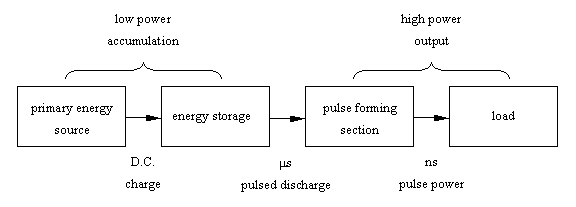
\includegraphics[height=4cm,width=8cm,keepaspectratio=true]{HPMsystem}
 \caption{Primjer ubacivanja slike.}
 \label{fig:prva}
	\end{center}
\end{figure}
\end{verbatim}
Uo�ite uporabu naredbe \verb|\label| unutar bloka. Na nju se potom u tekstu mo�emo referencirati pisanjem npr.\ \verb|Na Slici~\ref{fig:prva}| �ime \LaTeX{} u tekst uvrsti pripadaju�i broj slike, kao npr.\ ``Na Slici~\ref{fig:prva} prikazana je osnovna shema HPM sustava.''
Znak \verb|~| iza rije�i Slici osigurava to�no jedan znak razmaka, �to poma�e ukoliko je rije� Slika na kraju retka, da ne razdvoji rije� Slika i pripadaju�i broj slike.

\begin{figure}[!htbp]
	\begin{center}
 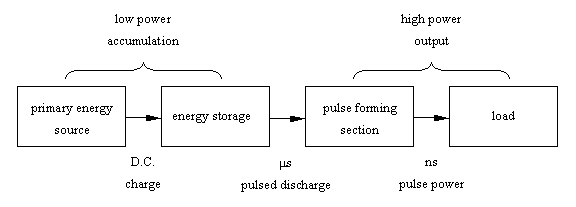
\includegraphics[height=4cm,width=8cm,keepaspectratio=true]{HPMsystem}
 \caption{Primjer ubacivanja slike.}
 \label{fig:prva}
	\end{center}
\end{figure}

Uo�ite i na�in prilago�avanja veli�ine slike. Parametri slike \emph{width} i \emph{height} odre�uju maksimalne dopu�tene dimenzije pri �emu se primarno po�tuje manju navedenu dimenziju, a \emph{keepaspectratio} osigurava zadr�avanje odnosa dimenzija slike, odnosno sprje�ava deformaciju slike, nakon proizvoljno unesenih veli�ina.

Uo�ite da sve oznake tj.\ \emph{labeli} ne smiju imati razmak u imenu. To vrijedi i op�enito, a ne samo za slike.

Tako�er, uo�ite da nije potrebno pisati ekstenziju slike jer to je ure�eno u postavkama glavnoga dokumenta pa time �tedi trud. Ekstenzije koje se mo�e izostaviti su: \emph{jpg}, \emph{jpeg}, \emph{png} i \emph{pdf}.

Shema prikazana na Slici~\ref{fig:prva} �e biti kori�tena i za potrebe idu�ih primjera, a {\color{blue} u mapi na va�em disku ju obri�ite nakon �to po�nete pohranjivati vlastite slike vezane uz va� rad}.


\section{Ubacivanje podslika}
Ponekada se jedna slika sastoji od dvije ili vi�e podslika kojima �elimo opisati neku cjelinu. Slika �e dobiti pripadni broj, a podslike slova (a), (b) itd.
To se mo�e posti�i sljede�om strukturom:
\begin{verbatim}
\begin{figure}[!htpb]
 \begin{center}
  \subfloat[Blok shema HPM sustava.]{\label{fig:HPM}
   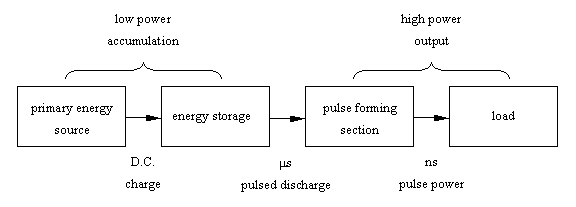
\includegraphics[height=5cm,width=10cm,keepaspectratio=true]{HPMsystem}}\\ 
	    %\hspace{10pt}
   \subfloat[JabRef su�elje za unos ``elektroni�ke'' reference.]
   {\label{fig:jabref}
   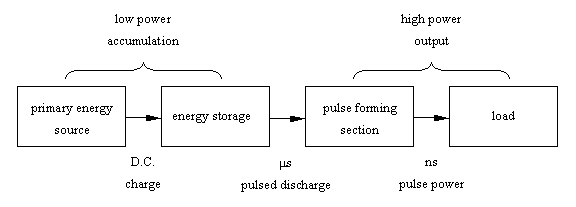
\includegraphics[height=7cm,keepaspectratio=true]{HPMsystem}}
\caption{Primjer ubacivanja vi�e podslika. Ovo je opis cijele slike.}
\label{fig:dvije_podslike}
  \end{center}
\end{figure}
\end{verbatim}
�to �e uvrstiti ono �to se vidi na Slici~\ref{fig:dvije_podslike}, koja se sastoji od dviju podslika.
Podslika~\ref{fig:HPM} pokazuje shemu HPM sustava, a podslika~\ref{fig:jabref} su�elje JabRef programa za unos bibliografskih jedinica.

\begin{figure}[!htpb]
	  \begin{center}
	   \subfloat[Blok shema HPM sustava.]{\label{fig:HPM} 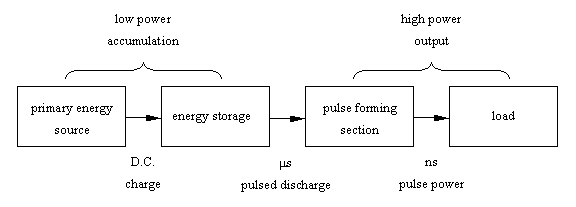
\includegraphics[height=5cm,width=10cm,keepaspectratio=true]{HPMsystem}} \\ %\hspace{10pt}
	   \subfloat[JabRef su�elje za unos ``elektroni�ke'' reference.]{\label{fig:jabref} 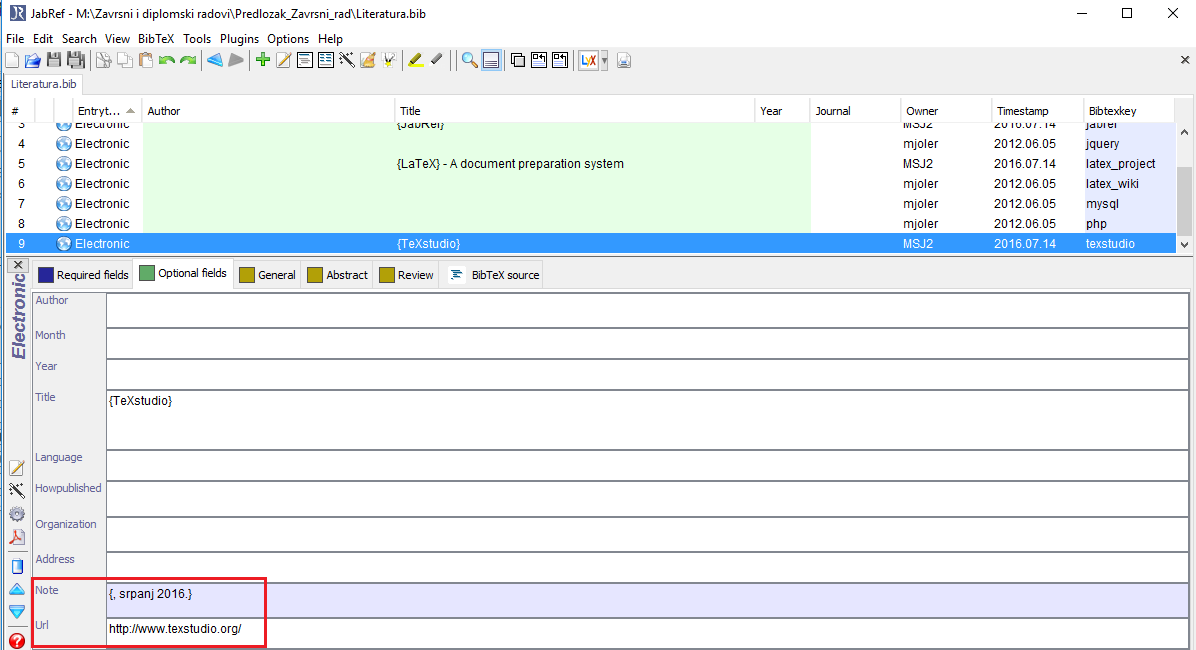
\includegraphics[height=7cm,keepaspectratio=true]{jabref}}
\caption{Primjer ubacivanja vi�e podslika. Ovo je opis cijele slike.}
\label{fig:dvije_podslike}
	  \end{center}
\end{figure}



\section{Ubacivanje tabele} 
Vi�e detalja o kreiranju tabela pro�itajte u literaturi, a sljede�i blok vam omogu�ava kreiranje jednostavne tabele, kao �to je prikazano u Tabeli~\ref{tab:prva}.
\begin{verbatim}
\begin{table}[!htbp]
\renewcommand{\arraystretch}{1.2}
\caption{Ovo je primjer izrade tabele.}
\centering
\begin{tabular}{|c|c|c|}
\hline
variabla & vrijednost 1 & vrijednost 2  \\ [0.5ex]
\hline \hline  
A & 5 & 3 \\ [0.5ex] % razmak do iducega retka
B & 4 & 2 \\ [0.5ex]
\hline
\end{tabular}
\label{tab:prva}
\end{table}
\end{verbatim}

\begin{table}[!htbp]
\renewcommand{\arraystretch}{1.2}
\caption{Ovo je primjer izrade tabele.}
\centering
\begin{tabular}{|c|c|c|}
\hline
variabla & vrijednost 1 & vrijednost 2  \\ [0.5ex]
\hline \hline 
A & 5 & 3 \\ [0.5ex] % razmak do iducega retka
B & 4 & 2 \\ [0.5ex]
\hline
\end{tabular}
\label{tab:prva}
\end{table}
%
Podaci koji su u stupcima se u tabeli razdvajaju znakom \&. Novi redak se na kraju aktualnoga retka formira znakom \verb|\\|. Broj stupaca se definira iza \emph{tabular} time �to se navedu slova koja ozna�avaju poravnavanje teksta u svakom stupcu, a broj slova zna�i broj stupaca koji �e biti kreiran u tabeli. Vertikalni razmak izme�u redaka u tabeli mo�ete za cijelu tabelu prilagoditi uporabom sljede�e sintakse prije strukture za tabelu:\\
\verb| \renewcommand{\arraystretch}{1.2} | gdje broj u zagradi na kraju (ovdje je 1.2) prilagodite sukladno va�oj preferenciji. Mo�e se prilagoditi i razmak za svaki pojedini redak (uo�ite \verb|[0.5ex]| na kraju redaka), ali to je manje od interesa jer tipi�no �elimo da svi retci imaju jednaki razmak jedni od drugih.

Sli�no mo�ete u�initi i za razmak izme�u stupaca tabele navo�enjem sljede�e sintakse prije bloka tabele:\\
\verb| \renewcommand{\tabcolsep}{0.3cm} |.



\section{Uporaba kratica u tekstu. Automatsko generiranje popisa kratica.}  \label{sec:kratice}
Listu kratica definirajte u datoteci \verb|Kratice.tex| (vidjeti predlo�ak unutar datoteke). U redovitom tekstu, kraticu  mo�ete ubaciti kori�tenjem naredbe \verb|\gls{ID_kratice}| gdje je \verb|ID_kraticE| identifikator kratice kako je definiran u datoteci \emph{Kratice.tex}. Pri prvoj uporabi naredbe \verb|\gls|, ispisat �e se najprije puni naziv pojma pa u zagradi kratica, a kod svake sljede�e uporabe, ispisat �e se samo kratica. Na primjer, kada (nakon prethodnog deklariranja u datoteci \verb|Kratice.tex|) upotrijebite \verb|\gls{gsm}| prvi puta, u tekstu �e se ispisati \gls{gsm}, a kada upotrijebite \verb|\gls{gsm}| drugi puta i dalje, u tekstu �e se ispisati samo \gls{gsm} (usporedi s definicijom kratice u datoteci \verb|Kratice.tex|). 
 
{\color{red} Listu kratica generirate sljede�im postupkom:} \label{generiranje_liste_kratica}
\begin{enumerate}
	\item Pokrenite kompilaciju cijeloga teksta jedanputa (to �e generirati neke datoteke koje su potrebne za daljnju obradu, specifi�no one s ekstenzijama .ist i .glo).
	\item Otvorite \emph{Command Prompt} aplikaciju na va�em ra�unalu i postavite se u radnu mapu gdje su vam datoteke za diplomski rad. 
	\item Potom pokrenite \emph{makeindex} rutinu (ona �e tipi�no biti ve� prisutna na va�em ra�unalu) upisuju�i sljede�u sintaksu: \\
	\verb|makeindex   -s myDoc.ist  -o myDoc.gls   myDoc.glo| \\
	gdje naziv datoteke \emph{myDoc} treba zamijeniti nazivom va�e glavne .tex datoteke, (npr. \verb|JMBAG_Ime_Prezime.tex|).
	\item Pokrenite \LaTeX{} jo� jednom ili dva puta, ako treba, dok se u uvodu pdf dokumenta ne pojavi lista kratica (pod naslovom \emph{Pojmovnik}).	
\end{enumerate}

Mo�da isprva zvu�i slo�eno, ali zapravo nije (bar ne uz ovako precizne upute!). Svaki puta kada dodate nove definicije kratica, potrebno je ponoviti ovaj postupak da bi se a�urirale odgovaraju�e datoteke i uredno prikazala potpuna lista u pdf-u (a i izbjegle poruke o pogre�kama tijekom kompajliranja teksta). 

Nije te�ko nakon �to prvi puta pro�ete ovaj postupak i omogu�ava vam u tekstu biti dosljedan u uporabi odre�ene kratice. Da izbjegnete �u�enje, va�no je jo� re�i da �e se ovim postupkom automatski stvoriti tek lista kratica koje ste u tekstu upotrijebili uporabom sintakse \verb|\gls|, a ne na temelju liste definicija koje ste naveli u datoteci \verb|Kratice.tex|. Zato, ako nijednom u tekstu ne upotrijebite sintaksu \verb|\gls|, ne�e biti ispisan ni popis kratica tj.\ \emph{Pojmovnik}. {\color{blue} Kako \LaTeX{} na kraju uvijek nagradi trud koji je ulo�en u savladavanje njegove sintakse, pogodnost ovakvoga automatskoga kreiranja Pojmovnika je i to �to uz svaki kraticu \LaTeX{} automatski ispi�e i brojeve stranica na kojima se doti�na kratica pojavljuje!} U elektroni�kom pdf dokumentu, brojevi stranica su ujedno i hiper-veze na te stranice pa se tako mo�e odmah sko�iti na stranicu gdje je pojedina kratica upotrijebljena.

Ukoliko vam se prethodno opisani postupak �ini preslo�enim, popis kratica mo�ete napraviti i ru�no, isto pomo�u datoteke Kratice.tex, u kojoj tako�er postoji kratki predlo�ak i za takav pristup. Za to je onda u osnovnoj datoteci \verb|JMBAG_Ima_Prezime.tex| potrebno deaktivirati liniju koda koja po�inje sa \verb|\printglossary|, a aktivirati blok koji po�inje sa \verb|\begin{glossary}| i zavr�ava sa \verb|end{glossary}|.



\section{Nagla�avanje teksta}
\subsection{Navodnici}
Za navodnike s lijeve strane fraze (otvaranje navodnika) koristi se 2x jednostruki navodnik koji se na tipkovnici nalazi lijevo od broja 1, a za navodnike s desne strane fraze (zatvaranje navodnika), koristi se 2x jednostruki navodnik koji se na tipkovnici nalazi na tipki \emph{�}, �to proizvede npr.\ ``abc''.

{\color{blue} Alternativno, u ovom paketu je pripremljena i naredba {\color{red} \verb|\navod{abc}|} gdje je \emph{abc} tekst koji se stavlja izme�u navodnika, tj.\ \navod{abc}.}

\subsection{Kosa i podebljana slova}
Nagla�avanje neke rije�i ili fraze pomo�u kosih (italic) slova mo�emo dobiti uporabom naredbe {\color{red} \verb|\emph{abc}|} ili pomo�u  {\color{red}\verb|\textit{abc}|} gdje je \emph{abc} neki tekst koji se �eli naglasiti.

\textbf{Podebljana slova} mo�emo posti�i uporabom naredbe {\color{red} \verb|\textbf{abc}|} gdje je \textit{abc} neki tekst koji �elimo podebljati.

\section{Verbatim: okru�enje za doslovni tekst}
Verbatim okru�enje omogu�ava ispis teksta u izvornom obliku, bez da ga \LaTeX{} tuma�i po svojiim sintakti�kim pravilima. To je pogodno kada se na stranicu  npr.\ �eli kopirati dio programskoga koda iz nekog jezika i kada �elimo zadr�ati sve izvorne znakove u nekoj frazi, bez da \LaTeX{} po�ne javljati pogre�ke kod kompajliranja, �to bi se moglo pojaviti kada se ne bi koristilo \emph{verbatim okru�enje}, po�to bi neke znakove interpretirao kao pogre�ke u sintaksi.

Postoji kra�i i du�i oblik verbatima. Kra�i slu�i za kra�u frazu od jedne ili par rije�i, a du�i za vi�e redaka.

\noindent Kra�i oblik verbatima ima sintaksu: \verb+\verb|neka fraza|+

\noindent Du�i oblik verbatima ima sintaksu:\\
\verb|\begin{verbatim}| \\
\verb|neki tekst| \\
\verb|\end{verbatim}| \\


\section{Kreiranje jedne jednad�be ili serije jednad�ba}

\subsection{Kreiranje jedne jednad�be}
Jednad�ba se napi�e u posebnom matemati�kom modu koji se kreira pomo�u bloka:
\begin{verbatim}
	\begin{equation}
		 A = B + C   \label{eq:prva}
	\end{equation}
\end{verbatim}
�to �e dati sljede�i izgled:
\begin{equation}
	 A = B + C   \label{eq:prva}
\end{equation}
Da bi se na nju referenciralo, na �eljenom mjestu u tekstu upi�emo \verb|\eqref{eq:prva}|, �ime �e se uvrstiti njezin pripadni (automatski generirani) broj, a za potpuniji smisao mo�emo npr.\ napisati \verb| Jednad�ba~\eqref{eq:prva}|, rezultat �ega je da �e u tekstu pisati Jednad�ba~\eqref{eq:prva}. 
Ako ju se ne �eli numerirati, onda se nakon rije�i \emph{begin} stavi zvjezdica, tj.\ \verb|begin*{equation}|.

\subsection{Kreiranje grupe jednad�ba}
Grupa jednad�ba se kreira uporabom \emph{subequations} sintakse. Na primjer, sljede�i blok �e definirati dvije podjednad�be u grupi, gdje �e svaka biti numerirana istim brojem, a razlikovati slovom iza broja.
\begin{verbatim}
	\begin{subequations}
		\begin{align}
		        A &= B + C  	\label{subeq:prva} \\
		        D &= F + G		\label{subeq:druga}
		\end{align}
	\label{subeq:obje}
	\end{subequations}
\end{verbatim}

To �e u izlaznom dokumentu rezultirati sljede�im izgledom:
\begin{subequations}
\begin{align}
        A &= B + C  	\label{subeq:prva} \\
        D &= F + G		\label{subeq:druga}
\end{align}
\label{subeq:obje}
\end{subequations}
U \eqref{subeq:prva} je prikazano dobivanje vrijednosti $A$, a u \eqref{subeq:druga} je prikazano dobivanje vrijednosti $D$. Jednad�ba~\eqref{subeq:obje} je \emph{�uveni studentov zakon}!



\section{Liste}
Liste su �este forme u tekstu kojima se na pregledni na�in nabrajaju neke stavke. Stavke obi�no navodimo ili s to�kama na po�etku, s brojevima ili sa slovima. U \LaTeX-u su upravo ta tri stila unaprijed definirana, a mogu�e su i slo�enije definicije stilova i kombinacije lista.

\subsection{Lista s to�kama}
Lista s to�kama se postigne blokom
\begin{verbatim}
\begin{itemize}
    \item prva nenumerirana stavka
    \item druga nenumerirana stavka
\end{itemize}
\end{verbatim}
�to na ekranu proizvede:
\begin{itemize}
% \setlength\itemsep{1ex}   % za lokalnu prilagodbu
	\item prva nenumerirana stavka
	\item druga nenumerirana stavka
\end{itemize}

\subsection{Lista s brojevima}
Numerirana lista s brojevima se postigne blokom
\begin{verbatim}
\begin{enumerate}[itemsep=1ex, topsep=4pt, partopsep=0pt]
     \item prva numerirana stavka
     \item druga numerirana stavka
\end{enumerate}
\end{verbatim}
U uglatoj zagradi su tri parametra kojima se to�no mo�e kontrolirati vertikalni razmak izme�u stavki u listi (\emph{itemsep}), razmak izme�u prethodnoga teksta i prve stavke u listi (\emph{topsep}) i dodatni prostor izme�u liste i prethodnoga paragrafa kada lista zapo�inje novi paragraf (\emph{partopsep}), ali te parametre \textbf{ne morate navoditi} tj.\ tu uglatu zagradu ne morate pisati. Tada �e se primijeniti vrijednosti parametara koje su definirane za cijeli dokument, a ove parametre se mo�e upotrijebiti tek da u nekom pojedinom slu�aju prilagodite razmake.
Za osjetiti efekte ovih parametara, najbolje se malo sam poigrati razli�itim vrijednostima parametara i vidjeti posljedice toga na listu (pri tome se uz brojeve kao prikladne jedinice za razmak mogu koristiti \emph{pt}, \emph{ex} ili \emph{em}).

\subsection{Proizvoljno ozna�ena lista}
Takva se lista mo�e posti�i u sklopu op�enitije forme koja omogu�uje proizvoljni opis ispred pojedine stavke, pomo�u sljede�ega bloka:
\begin{verbatim}
\begin{description}
     \item[a)] prva opisna stavka
     \item[b)] druga opisna stavka
\end{description}
\end{verbatim}
�to na ekranu proizvede:
\begin{description}%[itemsep=1ex, topsep=4pt, partopsep=0pt] za lokalnu prilagodbu
	\item[a)] prva opisna stavka
	\item[b)] druga opisna stavka \\
\end{description}
%
Kod ove strukture, u uglatu zagradu iza naredbe \verb|\item|, navodi se proizvoljna oznaka kojom se �eli na neki na�in ``numerirati'' listu.
%:::::::::::::::::::::::::::::::::::::::::::::::::::
\chapter{Dodatne informacije}
\section{Primjeri uporabe sintakti�kih struktura}
\begin{enumerate}
	\item Za uvid u kontekstualnu primjenu raznih sintakti�kih struktura, mo�ete otvoriti datoteku \href{run:Intro.tex}{{\color{blue}Intro.tex}}, unutar koje su napisane i ove upute. 
	\item Primjere slo�enijih sintakti�kih struktura, kao �to su ubacivanje slike, tabele ili jednad�be, mo�ete na�i u datoteci \href{run:sintaksa_cestih_struktura.tex}{{\color{blue}sintaksa\_cestih\_struktura.tex}} koja je dio paketa. Odabrane se strukture mo�e kopirati i zalijepiti u va� tekst, uz minimalne prilagodbe kao �to su naziv slike, veli�ina slike, opis i ID slike, a analogno i za tabele i jednad�be.
	\item Kona�no, za vi�e detalja o bilo �emu, potra�ite informacije u dvama priru�nicima koji su prilo�eni u mapi \href{run:prirucnici}{{\color{blue}prirucnici}} ili na webu, gdje se, me�u obiljem drugih informacija, nalaze i korisne wiki stranice \cite{latex_wiki,tex_exchange} o \LaTeX-u pomo�u kojih se obi�no brzo prona�e upute i zadovoljavaju�e rje�enje kakvom sintaksom se mo�e urediti �eljeni dio teksta.
\end{enumerate}

\section{Savjeti za lak�e ure�ivanje teksta}
Vjerujem da vam ovaj dokument mo�e uvelike pomo�i u pripremi teksta va�ega zavr�nog/diplomskog rada i omogu�iti da glavninu vremena tro�ite na sadr�aj rada, a manje na formatiranje rada jer to �e za vas sada obaviti \LaTeX{}! 

No, korektnosti radi, potrebno je napomenuti i sljede�e: \LaTeX{} je vrlo osjetljiv na pogre�ke u sintaksi naredbi (da, ba� kao �to su i programski jezici) pa vas mo�e povremeno ugnjaviti javljanjem pogre�ke koju nikako ne uspijevate uo�iti gdje je. Iskustvo kojim se izbjegava ta nelagoda jest sljede�e:
\begin{itemize}
	\item svako poglavlje napi�ite u novoj datoteci (da biste koli�inu teksta razdvojili na preglednije i manje cjeline) koju imenujte prikladnim imenom (bez razmaka u imenu). Potom te datoteke samo pozivajte iz glavnoga dokumenta \verb|JMBAG_Ime_Prezime.tex| pomo�u naredbe \verb|\include{ime_datoteke}|. Takav je pristup upravo i kori�ten u pripremi ovoga paketa.
	%
	\item {\color{red} budite koncentrirani dok pi�ete \LaTeX{} naredbe, poglavito zagrade, posebne znakove i matemati�ki tekst gdje se zahtijeva uporaba znaka \$!}
	%
	\item kompajlirajte tekst prije nego se skupi puno teksta jer tako �ete imati manje teksta za prekontrolirati u slu�aju pogre�ke. Tako�er vam za provjeru tek manjega dijela dokumenta mo�e pomo�i paket \verb|\usepackage{syntonly}| i naredba \verb|syntaxonly|, a isto tako i naredba \verb|\includeonly{ime_datoteke}| kojom �ete kompajlirati samo tu navedenu datoteku, �ime  ispred ``ne�eljenih'' datoteka ne morate stavljati znak ``komentara'' (\%).
	%
	\item ako niste sigurni ho�e li vam raditi neka naredba nakon pisanja, radije tekst kompajlirajte odmah po pisanju te naredbe---da vidite �to �ete dobiti i rije�ite dvojbu, nego da �ekate da se skupi jo� dubioznih mjesta u tekstu, kada �e nakon kompajliranja biti te�e detektirati koja linija teksta zapravo izaziva probleme (\LaTeX-ov prozor s porukama �esto nije odve� precizan u lociranju i opisu pogre�aka, ovisno o editoru teksta koji koristite).
\end{itemize}


\section{Zavr�ne napomene}
Ovime zaklju�ujemo uvodne upute koje �e najve�em broju studenata biti dovoljne (ili barem dovoljna osnova) za uspje�no pisanje zavr�nog odnosno diplomskog rada.

Prije nego prije�ete na kreiranje vlastitoga sadr�aja u�inite jo� sljede�e akcije kojima �ete deaktivirati dio paketa koji �e biti nepotreban:
\begin{enumerate}
	\item u mapi \href{run:slike}{{\color{blue}slike}}, obri�ite datoteke \verb|HPMsystem.png| i \verb|jabref.png| jer su one slu�ile tek za ilustracije u ovim Uputama.
	%
	\item u glavnoj datoteci  \href{run:JMBAG\_Ime\_Prezime.tex}{{\color{blue}JMBAG\_Ime\_Prezime.tex}} stavite znak komentara ``\%'' ispred linije \verb|\chapter{Kako koristiti paket za pisanje zavr�noga rada u \LaTeX-u}
Ovo su uvodne napomene za kori�tenje predlo�ka za pisanje zavr�noga ili diplomskoga rada studenata Tehni�koga fakulteta u Rijeci. Prije kori�tenja paketa, pro�itajte ovaj tekst jer �e vam dati nu�ne uvodne informacije, znatno vam olak�ati i ubrzati ure�ivanje teksta nakon toga, pri �emu �e vas i voditi kroz uporabu ovoga paketa na prakti�an na�in.

Paket je pripremljen tako da student �to prije mo�e pisati vlastiti tekst u ve� pripremljenom predlo�ku koji �e, uz minimalno u�enje sintakse \LaTeX-a, studentu olak�ati urediti svoj rad. U paketu su uklju�ene potrebne upute i sintakti�ke strukture koje bi trebale udovoljiti potrebama ve�ine studenta, a dodatne informacije postoje u dvama priru�nicima koji su uklju�eni u ovom paketu te, naravno, na raznim web stranicama na internetu koje su posve�ene \LaTeX-u (vidi u nastavku).

{\color{red} POZOR: paket treba biti prekopiran negdje na disk ne mijenjaju�i originalnu strukturu mapa (foldera) i ne mijenjaju�i nazive datoteka koje su u mapi \emph{tex\_aux}!}


\section{Opis sadr�aja paketa}
\vspace{-2ex}
Paket se sastoji od:
\begin{itemize}
 \item datoteke \href{run:UPUTE.pdf}{{\color{blue} UPUTE.pdf}} koja sadr�i postupak instalacije potrebnih alata na ra�unalo te kori�tenja paketa. \emph{UPUTE} su bazirane na Windows OS, a korisnici drugih OS-ova si na nazna�enim web lokacijama samo trebaju na�i instalacije za njihov OS.
 %
 \item datoteke \verb|JMBAG_Ime_Prezime.tex| koja je sredi�nja datoteka koja povezuje sve cjeline i kompajliranjem koje se dobije izlazni \verb|JMBAG_Ime_Prezime.pdf| dokument (naravno, tijekom rada, upisat �ete svoj specifi�ni JMBAG i ime i prezime).\\ U ovoj se datoteci inicijalno nalaze i upute za kori�tenje paketa kao i primjeri osnovne uporabe naj�e��ih sintakti�kih struktura u \LaTeX-u koje bi trebale biti dovoljne ve�ini studenata za pisanje rada.
 %
 \item mape \verb|tex_aux| u kojoj su \emph{interne datoteke} koje definiraju stilove, formate i sl.\ koji slu�e u slaganju izlaznoga formata. \textbf{Student/ica s njima ne treba \emph{ni�ta} raditi}, ali one trebaju biti u \verb|tex_aux| mapi pod glavnom mapom zavr�noga rada, kao �to je postavljeno u ovom paketu.
 %
 \item mape \emph{slike} u koju student treba pohraniti sve slike koje �e koristiti u radu. Ime mape se ne smije preimenovati bez boljega poznavanja sintakse \LaTeX-a jer ovaj paket da bi ispravno radio o�ekuje ba� takvo ime mape!
 %
 \item datoteke \verb|sintaksa_cestih_struktura.tex| koja ne sudjeluje izravno u kompajliranju pdf dokumenta, nego slu�i kao repozitorij u kojemu su sadr�ane naj�e��e potrebne sintakti�ke strukture koje su spremne za kopiranje u va� tekst uz minimalnu prilagodbu parametara (npr.\ opis slike, ime datoteke specifi�ne slike koju se ubacuje i proizvoljni ID te slike za kasnije referenciranje).
 %
 \item mape \href{run:prirucnici}{{\color{blue}prirucnici}} u kojoj se nalazi nekoliko najpopularnijih priru�nika za uporabu \LaTeX-a. 
\end{itemize}
%%%%%%%%%%%%%%%%%%%%%%%%%%%%%%%%%%%%%%%%%%%%%%%%%%%%%%%%%%%%%%%

\section{�ime se opremiti za pisanje rada}
Da bi se rad napisao pomo�u \LaTeX-a (a to vrijedi svake lipe!), najprije je na ra�unalo potrebno instalirati:
\begin{enumerate}
	\item obavezno: \LaTeX{} software 
	\item obavezno: editor za ure�ivanje teksta 
	\item neobavezno, ali korisno: softver za opis literature. (Premda dodatni softver nije nu�an jer se popis literature mo�e obraditi i ru�no (no to je manje sofisticirano kod uvr�tavanja referenca), sugeriram instalaciju softvera koji pomo�u intuitivnih su�elja korisniku omogu�ava opis pojedine kori�tene literature (kao mala baza podataka), a potom se pojedina jedinica literature jednostavno ubacuje u tekst, a popis literature se na kraju automatski formira (vi�e o tome pro�itajte u nastavku).
\end{enumerate}

\subsection{Instalacija \LaTeX-a}
\begin{enumerate}
	\item odite na sredi�nji \LaTeX{} portal \cite{latex_project}: \url{http://www.latex-project.org/}
	\item kliknite na poveznicu \href{http://www.latex-project.org/ftp.html}{Getting LaTeX} i potom uo�ite i povucite instalaciju koja odgovara va�em OS-u (npr.\ proTeXt za Windows, MacTeX za Mac, TeX Live za Linux). Pozor: instalacijski paket je velik i mo�e du�e potrajati �ak i na brzoj vezi---dajte si dovoljno vremena za obaviti download.
	\item Instalirajte \LaTeX{} slijede�i upute koje su prilo�ene za odabranu instalaciju (npr.\ proTeXt za Windowse daje kratki pdf s uputama koje vas vode kroz instalaciju korak po korak).
\end{enumerate}

\subsection{Instalacija editora teksta}
Instalirajte editor koji je pogodan za pisanje \LaTeX{} koda. \textbf{Za Windows OS, toplo preporu�am}  \href{http://www.texstudio.org}{{\color{blue} TeXstudio}} \cite{texstudio} jer je bogat opcijama, ugodan za rad i stabilan, a instalacije postoje i za Linux i Mac OS. TeXstudio se zasebno povu�e i instalira na ra�unalo, a neke editore teksta koji ve� do�u u paketu za instalaciju LaTeXa mo�ete ignorirati (npr.\ za Windows je do nedavno bio popularan \emph{TeXnicCenter} i dolazi ve� upakiran u proTeXt-u (a mo�da �ete na�i i \emph{TeXworks}), za Mac je kvalitetan \emph{TeXShop} koji sada tako�er dolazi u paketu s MacTeX-om). 

\label{encoding1} {\color{red} POZOR: Premda �e ovo biti jo� napomenuto na stranici~\pageref{encoding2}, prije samoga po�etka pisanja va�ega rada, �to prije �elim napomenuti sljede�i va�ni detalj: za svaki va� tekst koji pi�ete u editoru teksta, uvjerite se da je kodna stranica postavljena na \navod{windows-1250}, �to je klju�no da bi se u izlaznom pdf-u ispravno ispisivali hrvatski dijakriti�ki znakovi! U TeXstudiu, aktualnu kodnu stranicu se mo�e vidjeti i promijeniti preko maloga izbornika u doljnjem desnom kutu glavnoga prozora, gdje se nalazi opcija ``Encoding''. Ukoliko tu ne pi�e ``windows-1250'', kliknite na izbornik, odaberite opciju ``More Encodings'' pa u potom otvorenom su�elju odaberite kodnu stranicu ``windows-1250 / CP 1250'' i potvrdu sa ``Change To''.}

\subsection{Instalacija programa za opis kori�tene literature}
\emph{Ponavljamo: Kori�tenje BiBTeX programa za opis literature \textbf{nije} neophodno, ali jest korisno. U datoteci po imenu \href{run:Literatura.tex}{{\color{blue}Literatura.tex}}, koja je uklju�ena u ovaj paket, ve� su namje�tene postavke kao da �e se literatura opisati pomo�u BiBTeX programa (npr.\ JabRef-a) i ne treba ni�ta mijenjati, ali ispod toga se mo�e prona�i i upute i za drugi--ru�ni-- na�in (p)opisivanja literature.}

Kao bibtex program za opis literature, preporu�am \href{http://www.jabref.org}{{\color{blue} JabRef}} program \cite{jabref}. To je legalno besplatno dostupni program za Windows OS (ali postoji i za Mac, a i platformski neovisna instalacija) koji nam omogu�ava opisivanje literature na lak na�in pomo�u intuitivnih su�elja, a kao rezultat kreira \emph{BibTeX} datoteku \emph{Literatura.bib} (gdje je (\emph{Literatura} naziv koji korisnik treba dodijeliti pri pohrani JabRef datoteke na disk u slu�aju ovoga predlo�ka, da bi paket funkcionirao) u kojoj je literatura opisana na na�in koji \LaTeX{} razumije. 

Uo�ite da ako ne koristite JabRef, ve� se odlu�ite za ru�ni unos literature, �to se isprva doima jednostavnijim, tada �e vam redoslijed referenca u popisu literature odgovarati to�no redoslijedu koji ste naveli u tom popisu --- dakle morate paziti da redoslijed formirate onim redom kojim pozivate reference u va�em tekstu (�to kod nekog kasnije ubacivanja dodatne reference unutar ve� postoje�ega redoslijeda tra�i brigu da ju se ubaci na odgovaraju�e mjesto u popisu literature), a tako�er trebate paziti i na formatiranje teksta svake reference! 

Za razliku od toga, kori�tenjem JabRef-a, izbjegavate ru�no formiranje popisa literature i ne trebate brinuti o redoslijedu referenca, ve� samo pomo�u JabRefa trebate unijeti sve jedinice literature koju �ete navesti, a \LaTeX{} �e vam automatski formirati listu referenca onim redoslijedom kojim reference bude pozivali u tekstu!

Nakon �to kompajlirate projekt, stvorit �e vam se pomo�na datoteka imena \href{run:JMBAG_Ime_Prezime.bbl}{{\color{blue}JMBAG\_Ime\_Prezime.bbl}} u kojoj �e jedinice literature tijekom kompilacije biti formatirane i odatle se ubacuju u kona�nu verziju teksta. Stoga, \textbf{ukoliko ima ikakvih detalja koje u opisu literature treba prilagoditi, a ne mo�ete automatskim putem}, uvijek vam kao ``zadnja crta obrane'' ostaje otvoriti \verb|bbl| datoteku i tamo ru�no napraviti izmjene. Potom ponovo kompajlirajte projekt i te �e se promjene vidjeti u pdf-u tj.\ ru�no unijete promjene ne�e biti poni�tene sve dok ne obri�ete cijelu datoteku.

Umjesto da rukom pi�ete cijelu bibliografiju, vremenski vam je vjerojatno u�inko\-vitije popis literature generirate uporabom JabRef-a, a potom ako i�ta jo� treba prilagoditi, onda samo to napraviti ru�no u \verb|bbl| datoteci.


\subsubsection{Osnovna uporaba JabRef programa}
Upoznajte se s najva�nijim opcijama u \emph{JabRef}-u:
\begin{itemize}
	\item uo�ite ikonu (pod znakom ``+'' i tekstom \emph{New BibTeX Entry}) za unos nove jedinice literature (npr. knjige, �lanka, web portala i sl.)
	%
	\item kada kliknete za unos nove stavke literature, uo�ite kakvi se sve tipovi literature nude za odabir. Odabirom opcije koja odgovara naslovu koji �elite unijeti, otvorit �e vam se novi prozor s poljima u koja se mo�e unijeti informacije o literaturi. Za odabrani tip literature samo su neka polja obavezna (nalaze se pod karticom (eng.\ \emph{tabom}) \emph{Required fields}), dok se pod drugim karticama mo�e i ne mora unijeti dodatne informacije. U slu�aju na�ih zavr�nih/diplomskih radova, bit �e znatan udjeli literature koja je na internetu pa za formatiranje iste, pro�itajte upute i napomene u nastavku ove sekcije.
	%
	\item kada je vi�e autora, njihova imena se u JabRefu polju za unos autora razdvajaju pisanjem klju�ne rije�i \verb|and| (a ne razmakom, zarezom ili to�ka-zarezom!)
	%
	\item U popisu literature se ne�e uvijek pojam prepisati onako kako ste ga vi zapisali u JabRefu! To je posljedica stilova koji su definirani u \verb|bst| datoteci (ne zamarajte se time sada jer je za naprednu razinu \LaTeX-a). No, ako neki pojam ba� ne ispadne suvislo napisan u popisu literature ili ba� �elite forsirati odre�eni na�in zapisa (�esto slu�aj kada se rije� s velikim slovima ne interpretira onako kako �elite), tada to�no odre�eni zapis mo�ete forsirati na na�in da \verb|{tu rije� ili frazu stavite unutar viti�astih zagrada}|
	%
	\item prije nego pohranite pojedinu stavku pomo�u \emph{Ctrl+S}, \textbf{morate svakoj jedinici literature dodijeliti jedinstveni identifikator}, tzv.\ \emph{Bibtexkey}, �to je jedno od polja koja su obavezna za unos. Mo�ete ru�no upisati neki proizvoljni string, ali pogodnije je generirati ga automatski.\\ Za to u�initi me�u ikonama na vrhu imate ikonu koja izgleda kao (�arobni) �tapi� sa zvjezdicama oko njega, klikom na kojega \emph{JabRef} automatski dodijeli jedinstveni BibTeX \emph{klju�} za tu bibliografsku jedinicu. Pomo�u toga klju�a se poslije bilo kada i bilo gdje u pisanju va�ega rada mo�ete pozvati na tu referencu, a \LaTeX{} �e sve ostalo obaviti za vas tj.\ dodijeliti joj odgovaraju�i broj u tekstu i s tim brojem uvrstiti u popis literature.
	%
	\item korisnik ima mogu�nost i promijeniti uzorak po kojem se kreira struktura automatski generiranoga jedinstvenoga BibTeX klju�a tako da se otvori opcija izbornika \emph{Options $>>$ Preferences $>>$ BibTeX key generator}, gdje je na vrhu prozora prikazan \emph{default} uzorak, npr. \verb|[auth]:[year]| �to zna�i da se klju� kreira na bazi \verb|prezime(autora):godina(rada)|. To se sada mo�e urediti po nekom novom uzorku, no ovako definirani uzorak u biti zadovoljava, a ako igdje ima potrebe za dodatnim razlikovanjem, mo�e se na automatski generiranom klju�u jo� ru�no napraviti korekcija dodavanjem nekog znaka na kraju, kao npr.\ dodavanjem \verb|_a| i sl. (Klikom na karticu \emph{BibTeX source} mo�ete vidjeti kako �e unos va�ih podataka zapravo biti zapisan u va�oj \emph{Literatura.bib} datoteci koja �e se formirati od svih bibliografskih jedinica koje unesete.)
	%
	%
	\item Za \emph{ime} va�e bibliografske datoteke kod pohrane na disk obavezno upi�ite  \emph{Literatura} jer to ime o�ekuje ovaj paket. Pozor: Datoteka \emph{Literatura.bib}, koju ste tako kreirali, mora se nalaziti unutar mape ovoga paketa da bi sve ispravno radilo! U paketu je za primjer ve� kreirana jedna datoteka istoga imena koju za vje�bu student mo�e i otvoriti u \emph{JabRef}-u, ali to su samo pokazne bibliografske jedinice unesene kao primjer, koje student treba u kona�nici zamijeniti svojim bibliografskim jedinicama.
	%
	\item Za ``elektroni�ke'' izvore literature (tj.\ sve �to ste kao informaciju na�li na webu), JabRef nudi tip literature pod nazivom ``Electronic'' (vidi Sl.~\ref{fig:jabref}). U njemu pod karticom (eng.\ tabom) \emph{Optional fields} pod poljem \verb|Title| mo�ete upisati ime web stranice (autor, tvrtka i sl.), pod poljem \verb|url| mo�ete upisati URL adresu te web stranice, a pod poljem \verb|Note| upisati datum kada ste posjetili tu web stranicu (npr.\ \emph{srpanj 2016.} ili \emph{3.~rujna~2016.}). Rezultat toga �e u pdf-u biti da je sve napisano redoslijedom koji je predvi�en u Uputama RiTeha za pisanje diplomskog rada \cite{riteh_upute}, \emph{osim �to u ovom Predlo�ku do sada nisam uspio rije�iti ubacivanje zareza izme�u URL adrese i datuma posjeta toj URL adresi}, koji bi ta dva podatka odvojio, pa je tu potrebna mala ru�na \emph{prilagodba na jedan od ovih dvaju na�ina}:
	\begin{enumerate}[label=\textbf{\roman*)}]
		\item kod unosa datuma u polje \verb|Note| (u su�elju JabRef-a), upi�ite datum na sljede�i na�in: \verb|{, <datum>}|, gdje je \verb|<datum>| va� specifi�ni datum, dok �e \emph{zarez} iza prve zagrade izvr�iti razdvajanje URL adrese i datuma, a \textbf{viti�aste zagrade} osigurati da se to ba� tako to�no prenese u pdf-dokument (uklju�uju�i i da se mjesec napi�e malim po�etnim slovom, �to ina�e ne bi bio slu�aj). (Za neke druge tipove referenca kao npr.\ tip \emph{manual}, zarez vam prije datuma ne�e trebati jer �e naziv literature zavr�iti zarezom.) U Jabrefu vam i ina�e vrijedi da kada �elite forsirati da se pojam ba� to�no u popisu literature zapi�e onako kao ste htjeli, onda se pojam stavi unutar viti�astih zagrada \verb|{kao u ovom primjeru}|.
		\item ako u polju \verb|Note| ne upi�ete datum na prethodno opisani na�in, onda vam u pdf dokumentu ne�e biti upisan zarez izme�u URL adrese i datuma koji ste unijeli, a tako�er �e i mjesec biti napisan velikim po�etnim slovom (�to nije stra�no, ali je manje po�eljno). To mo�ete \emph{ru�no} prilagoditi tako da otvorite \verb|.bbl| datoteku i pomo�u \emph{Find/Replace} operacije sve nazive mjeseca zamijenite na na�in da po�inju malim po�etnim slovom (�to nije te�ko kada vam je ve�ina datuma u popisu literature navedena u istom mjesecu), ali zareze �ete svakako morati ubacivati ru�no u svaku pojedinu stavku literature jer ne�e biti nekog predlo�ka kojim biste to rije�ili automatski pomo�u \emph{Find/Replace} operacije. Na kraju opet kompajlirajte projekt. S obzirom na navedeno, prvi na�in je vremenski �tedljiviji!
	\end{enumerate}
\end{itemize}

%%%%%%%%%%%%%%%%%%%%%%%%%%%%%%%%%%%%%%%%%%%%%%%%%%%


\chapter{Primjeri naj�e��ih sintakti�kih struktura}
Prije stvarnoga po�etka pisanja svoga rada, upoznajte se s osnovnim sintakti�kim strukturama koje �e vam trebati tijekom pisanja rada.

U nastavku su opisane naj�e��e sintakti�ke strukture (dio njih mo�ete na�i i u datoteci \emph{Intro.tex}), a dodatne slo�enije strukture su pohranjene u datoteci \href{run:sintaksa_cestih_struktura.tex}{{\color{blue}sintaksa\_cestih\_struktura.tex}} koja je sastavni dio glave mape ovoga paketa. 

\section{Postavljanje naslova poglavlja i sekcija}
\begin{itemize}
	\item \verb|\chapter{Naslov poglavlja}|: za definiranje naslova poglavlja
	\item \verb|\section{Naslov sekcije}|: za definiranje naslova sekcije unutar poglavlja
	\item \verb|\subsection{Naslov podsekcije}|: za definiranje naslova podsekcije
\end{itemize}


\section{Reference na literaturu} \label{sec:RefLit}
Za referencu na pojedini kori�teni izvor informacije (tj.\ jedinicu literature), koristimo naredbu \\
\verb|\cite{bibtexkey}|, gdje je \emph{bibtexkey} jedinstveni klju� kojim prethodno ozna�imo tu jedinicu literature. \verb|Bibtexkey| mo�emo definirati na jedan od sljede�ih na�ina:
\begin{description}
	\item[I)] ako popis literature definiramo izravno u datoteci \href{run:Literatura.tex}{{\color{blue}Literatura.tex}} (opcija (I) u datoteci), onda ispred svake stavke literature treba definirati i jedinstveni \verb|bibtexkey| pomo�u naredbe \verb|\bibitem{bibtexkey}| (vidi predlo�ak u datoteci)
	\item[II)] ako literaturu opisujemo pomo�u JabRef datoteke \emph{Literatura.bib} (opcija (II) u datoteci), onda se tamo uz svaku stavku definira \verb|bibtexkey| (bude na dnu JabRef obrasca za upis pojedine jedinice literature)
\end{description}
%
Npr.\ ako negdje u tekstu napi�emo \verb|\cite{latex_wiki}|, gdje je \verb|latex_wiki| prethodno definirani \emph{bibtexkey}, tada �e se u tekstu u uglatoj zagradi pokazati broj  te bibliografske jedinice pod kojim se nalazi u popisu literature (Bibliografiji) na kraju rada (u ovom primjeru, to je broj \cite{latex_wiki}).


\section{Referenca na sekciju, sliku, tabelu ili stranicu} \label{sec:RefText}

Za referenciranje na pojedine dijelove teksta unutar rada, koristimo
{\color{red} \verb|\label{ID}|} i {\color{red} \verb|\ref{ID}|} na na�in da se \verb|\label{ID}| postavi uz dio teksta koji �elimo ozna�iti internom oznakom i poslije �emo se u tekstu na to referencirati, a \verb|\ref{ID}| upotrijebimo na mjestu s kojega se referenciramo na dio teksta koji je ranije ozna�en pomo�u \verb|\label{ID}|.

Ako se �elimo referencirati na specifi�nu sliku ili tabelu ili sekciju ili jednad�bu u tekstu, tada unutar bloka toga sadr�aja stavimo oznaku \verb|\label{prefiks:ID_objekta}| gdje je \emph{objekt} slika ili tablica ili sekcija teksta ili jednad�ba, a na �eljenom mjestu u tekstu se na to referiramo pomo�u \verb|\ref{prefiks:ID_objekta}| (u slu�aju referenciranja jednad�be, bolji oblik naredbe je {\color{red} \verb|\eqref{prefiks:ID_objekta}|}).

\verb|ID_objekta| je proizvoljni string (bez razmaka) koji dodijelimo objektu od interesa, a radi preglednijega ure�ivanja teksta, uobi�ajeno je u \LaTeX-u za pojedine tipove oznaka staviti i odgovaraju�i \emph{prefiks}, kao npr.\ \emph{sec} za oznaku sekcije, \emph{fig} za oznaku slike, \emph{tab} za oznaku tabele, \emph{eq} za oznaku jednad�be i sl. (Tako bi za sliku kojoj dodijelimo $ID=prva$ bilo \verb|\label{fig:prva}|, za tablicu \verb|\label{tab:prva}|, za sekciju \verb|\label{sec:prva}|, a za jednad�bu \verb|\label{eq:prva}|.)

Za referencirati se na \emph{stranicu} u tekstu gdje se nalazi ne�to na �to se �elite osvrnuti, koristi naredba {\color{red} \verb|\pageref{prefiks:ID_objekta}|}. Za njenu primjenu se tako�er prethodno treba ozna�iti �eljeni tekst pomo�u naredbe \verb|\label|.

Tako npr.\ mo�emo staviti da je primjer kreiranja tabele \emph{prva} opisan na stranici~\verb|\pageref{tab:prva}|, �to �e za rezultat imati tekst u kojem pi�e ``da je primjer kreiranja tabele \emph{prva} opisan na stranici~\pageref{tab:prva}'' (jer se u tekstu ta tabela nakon kompajliranja npr.\ na�e na stranici 12). Kako god se tekst smanjivao ili pove�avao i navedena tablica mijenjala broj stranice na kojoj se u kona�nici nalazi, mi ne moramo o tome brinuti jer \LaTeX{} brine o tome i na kraju napi�e to�ni broj stranice! (To je jo� jedna o pogodnosti zbog �ega se ljudi i odlu�e, uz ne�to po�etnoga truda, za kori�tenje \LaTeX-a!).



\section{Poveznica na neki dokument ili URL adresu}
Naredbe \verb|\url| i \verb|\href| slu�e za kreiranje poveznice na neku URL adresu ili neki dokument na disku.

{\color{red}\verb|\url{adresa}|} �e otisnuti URL adresu to�no onako kako je \emph{adresa} navedena unutar zagrada.

{\color{red}\verb|\href{akcija:destinacija}{opis}|} �e na papiru/ekranu ispisati tekst \emph{opis} koji je naveden u drugoj zagradi, i izvr�iti \emph{akciju} prema \emph{destinaciji} koja je navedena u prvoj zagradi. 
\emph{Akcija} mo�e npr.\ glasiti \emph{run} ili \emph{mailto}, gdje �e prvi oblik otvoriti mapu ili datoteku staza koje je navedena kao \emph{destinacija}, a drugi oblik pokrenuti pisanje emaila prema email adresi koja je navedena kao \emph{destinacija}.

Ne pretjerujte ipak s uporabom ovih struktura, odnosno uop�e ne morate to koristiti u radu, nego za vanjske reference koristiti samo \verb|\cite{bibtexkey}| naredbu, a za unutra�nje reference (na dijelove teksta) kombinaciju naredbi \verb|\label{ID}| i \verb|\ref{ID}| kako je to opisano u Sekciji~\ref{sec:RefText}. 


\section{Ubacivanje slike}
Sliku mo�emo ubaciti pomo�u sljede�ega bloka naredbi:
\begin{verbatim}
\begin{figure}[!htbp]
	\begin{center}
 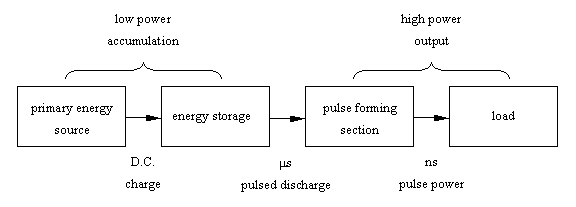
\includegraphics[height=4cm,width=8cm,keepaspectratio=true]{HPMsystem}
 \caption{Primjer ubacivanja slike.}
 \label{fig:prva}
	\end{center}
\end{figure}
\end{verbatim}
Uo�ite uporabu naredbe \verb|\label| unutar bloka. Na nju se potom u tekstu mo�emo referencirati pisanjem npr.\ \verb|Na Slici~\ref{fig:prva}| �ime \LaTeX{} u tekst uvrsti pripadaju�i broj slike, kao npr.\ ``Na Slici~\ref{fig:prva} prikazana je osnovna shema HPM sustava.''
Znak \verb|~| iza rije�i Slici osigurava to�no jedan znak razmaka, �to poma�e ukoliko je rije� Slika na kraju retka, da ne razdvoji rije� Slika i pripadaju�i broj slike.

\begin{figure}[!htbp]
	\begin{center}
 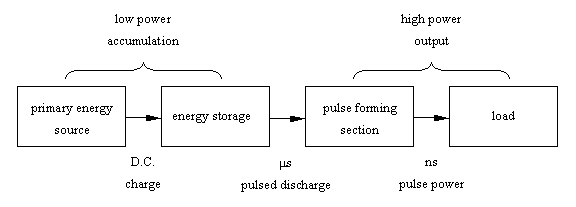
\includegraphics[height=4cm,width=8cm,keepaspectratio=true]{HPMsystem}
 \caption{Primjer ubacivanja slike.}
 \label{fig:prva}
	\end{center}
\end{figure}

Uo�ite i na�in prilago�avanja veli�ine slike. Parametri slike \emph{width} i \emph{height} odre�uju maksimalne dopu�tene dimenzije pri �emu se primarno po�tuje manju navedenu dimenziju, a \emph{keepaspectratio} osigurava zadr�avanje odnosa dimenzija slike, odnosno sprje�ava deformaciju slike, nakon proizvoljno unesenih veli�ina.

Uo�ite da sve oznake tj.\ \emph{labeli} ne smiju imati razmak u imenu. To vrijedi i op�enito, a ne samo za slike.

Tako�er, uo�ite da nije potrebno pisati ekstenziju slike jer to je ure�eno u postavkama glavnoga dokumenta pa time �tedi trud. Ekstenzije koje se mo�e izostaviti su: \emph{jpg}, \emph{jpeg}, \emph{png} i \emph{pdf}.

Shema prikazana na Slici~\ref{fig:prva} �e biti kori�tena i za potrebe idu�ih primjera, a {\color{blue} u mapi na va�em disku ju obri�ite nakon �to po�nete pohranjivati vlastite slike vezane uz va� rad}.


\section{Ubacivanje podslika}
Ponekada se jedna slika sastoji od dvije ili vi�e podslika kojima �elimo opisati neku cjelinu. Slika �e dobiti pripadni broj, a podslike slova (a), (b) itd.
To se mo�e posti�i sljede�om strukturom:
\begin{verbatim}
\begin{figure}[!htpb]
 \begin{center}
  \subfloat[Blok shema HPM sustava.]{\label{fig:HPM}
   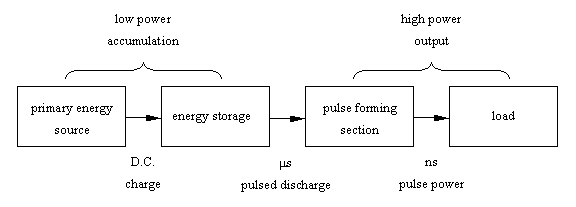
\includegraphics[height=5cm,width=10cm,keepaspectratio=true]{HPMsystem}}\\ 
	    %\hspace{10pt}
   \subfloat[JabRef su�elje za unos ``elektroni�ke'' reference.]
   {\label{fig:jabref}
   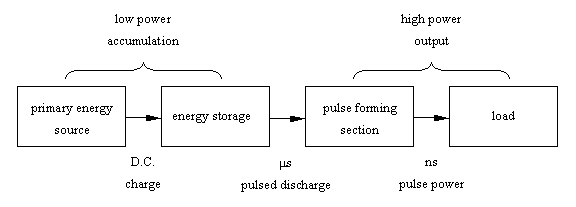
\includegraphics[height=7cm,keepaspectratio=true]{HPMsystem}}
\caption{Primjer ubacivanja vi�e podslika. Ovo je opis cijele slike.}
\label{fig:dvije_podslike}
  \end{center}
\end{figure}
\end{verbatim}
�to �e uvrstiti ono �to se vidi na Slici~\ref{fig:dvije_podslike}, koja se sastoji od dviju podslika.
Podslika~\ref{fig:HPM} pokazuje shemu HPM sustava, a podslika~\ref{fig:jabref} su�elje JabRef programa za unos bibliografskih jedinica.

\begin{figure}[!htpb]
	  \begin{center}
	   \subfloat[Blok shema HPM sustava.]{\label{fig:HPM} 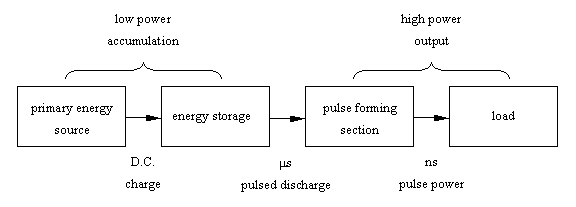
\includegraphics[height=5cm,width=10cm,keepaspectratio=true]{HPMsystem}} \\ %\hspace{10pt}
	   \subfloat[JabRef su�elje za unos ``elektroni�ke'' reference.]{\label{fig:jabref} 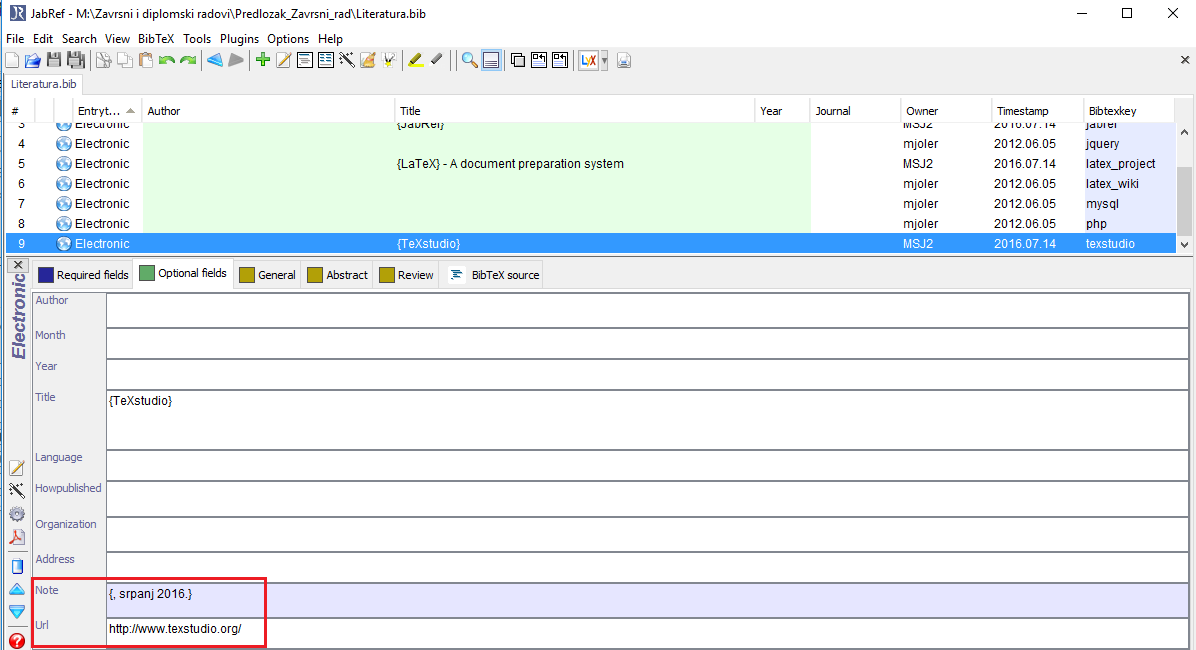
\includegraphics[height=7cm,keepaspectratio=true]{jabref}}
\caption{Primjer ubacivanja vi�e podslika. Ovo je opis cijele slike.}
\label{fig:dvije_podslike}
	  \end{center}
\end{figure}



\section{Ubacivanje tabele} 
Vi�e detalja o kreiranju tabela pro�itajte u literaturi, a sljede�i blok vam omogu�ava kreiranje jednostavne tabele, kao �to je prikazano u Tabeli~\ref{tab:prva}.
\begin{verbatim}
\begin{table}[!htbp]
\renewcommand{\arraystretch}{1.2}
\caption{Ovo je primjer izrade tabele.}
\centering
\begin{tabular}{|c|c|c|}
\hline
variabla & vrijednost 1 & vrijednost 2  \\ [0.5ex]
\hline \hline  
A & 5 & 3 \\ [0.5ex] % razmak do iducega retka
B & 4 & 2 \\ [0.5ex]
\hline
\end{tabular}
\label{tab:prva}
\end{table}
\end{verbatim}

\begin{table}[!htbp]
\renewcommand{\arraystretch}{1.2}
\caption{Ovo je primjer izrade tabele.}
\centering
\begin{tabular}{|c|c|c|}
\hline
variabla & vrijednost 1 & vrijednost 2  \\ [0.5ex]
\hline \hline 
A & 5 & 3 \\ [0.5ex] % razmak do iducega retka
B & 4 & 2 \\ [0.5ex]
\hline
\end{tabular}
\label{tab:prva}
\end{table}
%
Podaci koji su u stupcima se u tabeli razdvajaju znakom \&. Novi redak se na kraju aktualnoga retka formira znakom \verb|\\|. Broj stupaca se definira iza \emph{tabular} time �to se navedu slova koja ozna�avaju poravnavanje teksta u svakom stupcu, a broj slova zna�i broj stupaca koji �e biti kreiran u tabeli. Vertikalni razmak izme�u redaka u tabeli mo�ete za cijelu tabelu prilagoditi uporabom sljede�e sintakse prije strukture za tabelu:\\
\verb| \renewcommand{\arraystretch}{1.2} | gdje broj u zagradi na kraju (ovdje je 1.2) prilagodite sukladno va�oj preferenciji. Mo�e se prilagoditi i razmak za svaki pojedini redak (uo�ite \verb|[0.5ex]| na kraju redaka), ali to je manje od interesa jer tipi�no �elimo da svi retci imaju jednaki razmak jedni od drugih.

Sli�no mo�ete u�initi i za razmak izme�u stupaca tabele navo�enjem sljede�e sintakse prije bloka tabele:\\
\verb| \renewcommand{\tabcolsep}{0.3cm} |.



\section{Uporaba kratica u tekstu. Automatsko generiranje popisa kratica.}  \label{sec:kratice}
Listu kratica definirajte u datoteci \verb|Kratice.tex| (vidjeti predlo�ak unutar datoteke). U redovitom tekstu, kraticu  mo�ete ubaciti kori�tenjem naredbe \verb|\gls{ID_kratice}| gdje je \verb|ID_kraticE| identifikator kratice kako je definiran u datoteci \emph{Kratice.tex}. Pri prvoj uporabi naredbe \verb|\gls|, ispisat �e se najprije puni naziv pojma pa u zagradi kratica, a kod svake sljede�e uporabe, ispisat �e se samo kratica. Na primjer, kada (nakon prethodnog deklariranja u datoteci \verb|Kratice.tex|) upotrijebite \verb|\gls{gsm}| prvi puta, u tekstu �e se ispisati \gls{gsm}, a kada upotrijebite \verb|\gls{gsm}| drugi puta i dalje, u tekstu �e se ispisati samo \gls{gsm} (usporedi s definicijom kratice u datoteci \verb|Kratice.tex|). 
 
{\color{red} Listu kratica generirate sljede�im postupkom:} \label{generiranje_liste_kratica}
\begin{enumerate}
	\item Pokrenite kompilaciju cijeloga teksta jedanputa (to �e generirati neke datoteke koje su potrebne za daljnju obradu, specifi�no one s ekstenzijama .ist i .glo).
	\item Otvorite \emph{Command Prompt} aplikaciju na va�em ra�unalu i postavite se u radnu mapu gdje su vam datoteke za diplomski rad. 
	\item Potom pokrenite \emph{makeindex} rutinu (ona �e tipi�no biti ve� prisutna na va�em ra�unalu) upisuju�i sljede�u sintaksu: \\
	\verb|makeindex   -s myDoc.ist  -o myDoc.gls   myDoc.glo| \\
	gdje naziv datoteke \emph{myDoc} treba zamijeniti nazivom va�e glavne .tex datoteke, (npr. \verb|JMBAG_Ime_Prezime.tex|).
	\item Pokrenite \LaTeX{} jo� jednom ili dva puta, ako treba, dok se u uvodu pdf dokumenta ne pojavi lista kratica (pod naslovom \emph{Pojmovnik}).	
\end{enumerate}

Mo�da isprva zvu�i slo�eno, ali zapravo nije (bar ne uz ovako precizne upute!). Svaki puta kada dodate nove definicije kratica, potrebno je ponoviti ovaj postupak da bi se a�urirale odgovaraju�e datoteke i uredno prikazala potpuna lista u pdf-u (a i izbjegle poruke o pogre�kama tijekom kompajliranja teksta). 

Nije te�ko nakon �to prvi puta pro�ete ovaj postupak i omogu�ava vam u tekstu biti dosljedan u uporabi odre�ene kratice. Da izbjegnete �u�enje, va�no je jo� re�i da �e se ovim postupkom automatski stvoriti tek lista kratica koje ste u tekstu upotrijebili uporabom sintakse \verb|\gls|, a ne na temelju liste definicija koje ste naveli u datoteci \verb|Kratice.tex|. Zato, ako nijednom u tekstu ne upotrijebite sintaksu \verb|\gls|, ne�e biti ispisan ni popis kratica tj.\ \emph{Pojmovnik}. {\color{blue} Kako \LaTeX{} na kraju uvijek nagradi trud koji je ulo�en u savladavanje njegove sintakse, pogodnost ovakvoga automatskoga kreiranja Pojmovnika je i to �to uz svaki kraticu \LaTeX{} automatski ispi�e i brojeve stranica na kojima se doti�na kratica pojavljuje!} U elektroni�kom pdf dokumentu, brojevi stranica su ujedno i hiper-veze na te stranice pa se tako mo�e odmah sko�iti na stranicu gdje je pojedina kratica upotrijebljena.

Ukoliko vam se prethodno opisani postupak �ini preslo�enim, popis kratica mo�ete napraviti i ru�no, isto pomo�u datoteke Kratice.tex, u kojoj tako�er postoji kratki predlo�ak i za takav pristup. Za to je onda u osnovnoj datoteci \verb|JMBAG_Ima_Prezime.tex| potrebno deaktivirati liniju koda koja po�inje sa \verb|\printglossary|, a aktivirati blok koji po�inje sa \verb|\begin{glossary}| i zavr�ava sa \verb|end{glossary}|.



\section{Nagla�avanje teksta}
\subsection{Navodnici}
Za navodnike s lijeve strane fraze (otvaranje navodnika) koristi se 2x jednostruki navodnik koji se na tipkovnici nalazi lijevo od broja 1, a za navodnike s desne strane fraze (zatvaranje navodnika), koristi se 2x jednostruki navodnik koji se na tipkovnici nalazi na tipki \emph{�}, �to proizvede npr.\ ``abc''.

{\color{blue} Alternativno, u ovom paketu je pripremljena i naredba {\color{red} \verb|\navod{abc}|} gdje je \emph{abc} tekst koji se stavlja izme�u navodnika, tj.\ \navod{abc}.}

\subsection{Kosa i podebljana slova}
Nagla�avanje neke rije�i ili fraze pomo�u kosih (italic) slova mo�emo dobiti uporabom naredbe {\color{red} \verb|\emph{abc}|} ili pomo�u  {\color{red}\verb|\textit{abc}|} gdje je \emph{abc} neki tekst koji se �eli naglasiti.

\textbf{Podebljana slova} mo�emo posti�i uporabom naredbe {\color{red} \verb|\textbf{abc}|} gdje je \textit{abc} neki tekst koji �elimo podebljati.

\section{Verbatim: okru�enje za doslovni tekst}
Verbatim okru�enje omogu�ava ispis teksta u izvornom obliku, bez da ga \LaTeX{} tuma�i po svojiim sintakti�kim pravilima. To je pogodno kada se na stranicu  npr.\ �eli kopirati dio programskoga koda iz nekog jezika i kada �elimo zadr�ati sve izvorne znakove u nekoj frazi, bez da \LaTeX{} po�ne javljati pogre�ke kod kompajliranja, �to bi se moglo pojaviti kada se ne bi koristilo \emph{verbatim okru�enje}, po�to bi neke znakove interpretirao kao pogre�ke u sintaksi.

Postoji kra�i i du�i oblik verbatima. Kra�i slu�i za kra�u frazu od jedne ili par rije�i, a du�i za vi�e redaka.

\noindent Kra�i oblik verbatima ima sintaksu: \verb+\verb|neka fraza|+

\noindent Du�i oblik verbatima ima sintaksu:\\
\verb|\begin{verbatim}| \\
\verb|neki tekst| \\
\verb|\end{verbatim}| \\


\section{Kreiranje jedne jednad�be ili serije jednad�ba}

\subsection{Kreiranje jedne jednad�be}
Jednad�ba se napi�e u posebnom matemati�kom modu koji se kreira pomo�u bloka:
\begin{verbatim}
	\begin{equation}
		 A = B + C   \label{eq:prva}
	\end{equation}
\end{verbatim}
�to �e dati sljede�i izgled:
\begin{equation}
	 A = B + C   \label{eq:prva}
\end{equation}
Da bi se na nju referenciralo, na �eljenom mjestu u tekstu upi�emo \verb|\eqref{eq:prva}|, �ime �e se uvrstiti njezin pripadni (automatski generirani) broj, a za potpuniji smisao mo�emo npr.\ napisati \verb| Jednad�ba~\eqref{eq:prva}|, rezultat �ega je da �e u tekstu pisati Jednad�ba~\eqref{eq:prva}. 
Ako ju se ne �eli numerirati, onda se nakon rije�i \emph{begin} stavi zvjezdica, tj.\ \verb|begin*{equation}|.

\subsection{Kreiranje grupe jednad�ba}
Grupa jednad�ba se kreira uporabom \emph{subequations} sintakse. Na primjer, sljede�i blok �e definirati dvije podjednad�be u grupi, gdje �e svaka biti numerirana istim brojem, a razlikovati slovom iza broja.
\begin{verbatim}
	\begin{subequations}
		\begin{align}
		        A &= B + C  	\label{subeq:prva} \\
		        D &= F + G		\label{subeq:druga}
		\end{align}
	\label{subeq:obje}
	\end{subequations}
\end{verbatim}

To �e u izlaznom dokumentu rezultirati sljede�im izgledom:
\begin{subequations}
\begin{align}
        A &= B + C  	\label{subeq:prva} \\
        D &= F + G		\label{subeq:druga}
\end{align}
\label{subeq:obje}
\end{subequations}
U \eqref{subeq:prva} je prikazano dobivanje vrijednosti $A$, a u \eqref{subeq:druga} je prikazano dobivanje vrijednosti $D$. Jednad�ba~\eqref{subeq:obje} je \emph{�uveni studentov zakon}!



\section{Liste}
Liste su �este forme u tekstu kojima se na pregledni na�in nabrajaju neke stavke. Stavke obi�no navodimo ili s to�kama na po�etku, s brojevima ili sa slovima. U \LaTeX-u su upravo ta tri stila unaprijed definirana, a mogu�e su i slo�enije definicije stilova i kombinacije lista.

\subsection{Lista s to�kama}
Lista s to�kama se postigne blokom
\begin{verbatim}
\begin{itemize}
    \item prva nenumerirana stavka
    \item druga nenumerirana stavka
\end{itemize}
\end{verbatim}
�to na ekranu proizvede:
\begin{itemize}
% \setlength\itemsep{1ex}   % za lokalnu prilagodbu
	\item prva nenumerirana stavka
	\item druga nenumerirana stavka
\end{itemize}

\subsection{Lista s brojevima}
Numerirana lista s brojevima se postigne blokom
\begin{verbatim}
\begin{enumerate}[itemsep=1ex, topsep=4pt, partopsep=0pt]
     \item prva numerirana stavka
     \item druga numerirana stavka
\end{enumerate}
\end{verbatim}
U uglatoj zagradi su tri parametra kojima se to�no mo�e kontrolirati vertikalni razmak izme�u stavki u listi (\emph{itemsep}), razmak izme�u prethodnoga teksta i prve stavke u listi (\emph{topsep}) i dodatni prostor izme�u liste i prethodnoga paragrafa kada lista zapo�inje novi paragraf (\emph{partopsep}), ali te parametre \textbf{ne morate navoditi} tj.\ tu uglatu zagradu ne morate pisati. Tada �e se primijeniti vrijednosti parametara koje su definirane za cijeli dokument, a ove parametre se mo�e upotrijebiti tek da u nekom pojedinom slu�aju prilagodite razmake.
Za osjetiti efekte ovih parametara, najbolje se malo sam poigrati razli�itim vrijednostima parametara i vidjeti posljedice toga na listu (pri tome se uz brojeve kao prikladne jedinice za razmak mogu koristiti \emph{pt}, \emph{ex} ili \emph{em}).

\subsection{Proizvoljno ozna�ena lista}
Takva se lista mo�e posti�i u sklopu op�enitije forme koja omogu�uje proizvoljni opis ispred pojedine stavke, pomo�u sljede�ega bloka:
\begin{verbatim}
\begin{description}
     \item[a)] prva opisna stavka
     \item[b)] druga opisna stavka
\end{description}
\end{verbatim}
�to na ekranu proizvede:
\begin{description}%[itemsep=1ex, topsep=4pt, partopsep=0pt] za lokalnu prilagodbu
	\item[a)] prva opisna stavka
	\item[b)] druga opisna stavka \\
\end{description}
%
Kod ove strukture, u uglatu zagradu iza naredbe \verb|\item|, navodi se proizvoljna oznaka kojom se �eli na neki na�in ``numerirati'' listu.
%:::::::::::::::::::::::::::::::::::::::::::::::::::
\chapter{Dodatne informacije}
\section{Primjeri uporabe sintakti�kih struktura}
\begin{enumerate}
	\item Za uvid u kontekstualnu primjenu raznih sintakti�kih struktura, mo�ete otvoriti datoteku \href{run:Intro.tex}{{\color{blue}Intro.tex}}, unutar koje su napisane i ove upute. 
	\item Primjere slo�enijih sintakti�kih struktura, kao �to su ubacivanje slike, tabele ili jednad�be, mo�ete na�i u datoteci \href{run:sintaksa_cestih_struktura.tex}{{\color{blue}sintaksa\_cestih\_struktura.tex}} koja je dio paketa. Odabrane se strukture mo�e kopirati i zalijepiti u va� tekst, uz minimalne prilagodbe kao �to su naziv slike, veli�ina slike, opis i ID slike, a analogno i za tabele i jednad�be.
	\item Kona�no, za vi�e detalja o bilo �emu, potra�ite informacije u dvama priru�nicima koji su prilo�eni u mapi \href{run:prirucnici}{{\color{blue}prirucnici}} ili na webu, gdje se, me�u obiljem drugih informacija, nalaze i korisne wiki stranice \cite{latex_wiki,tex_exchange} o \LaTeX-u pomo�u kojih se obi�no brzo prona�e upute i zadovoljavaju�e rje�enje kakvom sintaksom se mo�e urediti �eljeni dio teksta.
\end{enumerate}

\section{Savjeti za lak�e ure�ivanje teksta}
Vjerujem da vam ovaj dokument mo�e uvelike pomo�i u pripremi teksta va�ega zavr�nog/diplomskog rada i omogu�iti da glavninu vremena tro�ite na sadr�aj rada, a manje na formatiranje rada jer to �e za vas sada obaviti \LaTeX{}! 

No, korektnosti radi, potrebno je napomenuti i sljede�e: \LaTeX{} je vrlo osjetljiv na pogre�ke u sintaksi naredbi (da, ba� kao �to su i programski jezici) pa vas mo�e povremeno ugnjaviti javljanjem pogre�ke koju nikako ne uspijevate uo�iti gdje je. Iskustvo kojim se izbjegava ta nelagoda jest sljede�e:
\begin{itemize}
	\item svako poglavlje napi�ite u novoj datoteci (da biste koli�inu teksta razdvojili na preglednije i manje cjeline) koju imenujte prikladnim imenom (bez razmaka u imenu). Potom te datoteke samo pozivajte iz glavnoga dokumenta \verb|JMBAG_Ime_Prezime.tex| pomo�u naredbe \verb|\include{ime_datoteke}|. Takav je pristup upravo i kori�ten u pripremi ovoga paketa.
	%
	\item {\color{red} budite koncentrirani dok pi�ete \LaTeX{} naredbe, poglavito zagrade, posebne znakove i matemati�ki tekst gdje se zahtijeva uporaba znaka \$!}
	%
	\item kompajlirajte tekst prije nego se skupi puno teksta jer tako �ete imati manje teksta za prekontrolirati u slu�aju pogre�ke. Tako�er vam za provjeru tek manjega dijela dokumenta mo�e pomo�i paket \verb|\usepackage{syntonly}| i naredba \verb|syntaxonly|, a isto tako i naredba \verb|\includeonly{ime_datoteke}| kojom �ete kompajlirati samo tu navedenu datoteku, �ime  ispred ``ne�eljenih'' datoteka ne morate stavljati znak ``komentara'' (\%).
	%
	\item ako niste sigurni ho�e li vam raditi neka naredba nakon pisanja, radije tekst kompajlirajte odmah po pisanju te naredbe---da vidite �to �ete dobiti i rije�ite dvojbu, nego da �ekate da se skupi jo� dubioznih mjesta u tekstu, kada �e nakon kompajliranja biti te�e detektirati koja linija teksta zapravo izaziva probleme (\LaTeX-ov prozor s porukama �esto nije odve� precizan u lociranju i opisu pogre�aka, ovisno o editoru teksta koji koristite).
\end{itemize}


\section{Zavr�ne napomene}
Ovime zaklju�ujemo uvodne upute koje �e najve�em broju studenata biti dovoljne (ili barem dovoljna osnova) za uspje�no pisanje zavr�nog odnosno diplomskog rada.

Prije nego prije�ete na kreiranje vlastitoga sadr�aja u�inite jo� sljede�e akcije kojima �ete deaktivirati dio paketa koji �e biti nepotreban:
\begin{enumerate}
	\item u mapi \href{run:slike}{{\color{blue}slike}}, obri�ite datoteke \verb|HPMsystem.png| i \verb|jabref.png| jer su one slu�ile tek za ilustracije u ovim Uputama.
	%
	\item u glavnoj datoteci  \href{run:JMBAG\_Ime\_Prezime.tex}{{\color{blue}JMBAG\_Ime\_Prezime.tex}} stavite znak komentara ``\%'' ispred linije \verb|\include{Intro}| kojom se pozivaju ove upute ili obri�ite tu liniju koda, �ime to vi�e ne�e biti uklju�eno u tekst va�eg vlastitoga rada.
\end{enumerate}

Budite slobodni emailati svoje dojmove o razumljivosti i prakti�nosti ovoga materijala, kao i informacije o uo�enim pogre�kama u tekstu. \\

\noindent Ugodan rad! \\

\noindent Miroslav Joler	\\	
\href{mailto:mjoler@riteh.hr}{mjoler@riteh.hr}	\\ \\


{\color{red} A sada, prije�ite na kreiranje vlastitoga sadr�aja, pri �emu �e vam, za po�etak, pomo�i vodi� iz sljede�ega poglavlja.}


\chapter{Vodi� za pisanje vlastitoga teksta}

\section{Upis uvodnih podataka}
\begin{enumerate}
	\item {\color{red} \textbf{Otvaranje glavne datoteke.}} Pokrenite va� editor \LaTeX{} teksta i iz njega otvorite sredi�nju datoteku ovoga predlo�ka za pisanje rada, koja je nazvana \href{run:JMBAG\_Ime\_Prezime.tex}{{\color{blue}JMBAG\_Ime\_Prezime.tex}} i nalazi se u sredi�njoj mapi unutar ovoga paketa (ili probajte klikom na prethodnu poveznicu u tekstu).
	%
	\item {\color{red} \textbf{Upis uvodnih podataka.}} U gornjem dijelu dokumenta nemate ni�ta za mijenjati, nego skrolajte prema dolje do linije koja glasi: \verb|\begin{document}|. Specifi�ni podaci koje student/ica nakon toga treba upisati bit �e uz sljede�e naredbe:
	\begin{itemize}
		\item \verb|\degreesubject|: upisati razinu studija koji poha�ate (npr.\ Preddiplomski studij ra�unarstva ili Diplomski studij ra�unarstva i sl.)
		\item \verb|\documenttype|: upisati \emph{Zavr�ni rad} ili \emph{Diplomski rad}
		\item \verb|\title|: upisati naslov rada kako je zadano u slu�benom zadatku
%\item \verb|\date|: upisati samo mjesec predaje rada. Godina se upisuje automatski.
		\item \verb|\author|: upisati svoje ime i prezime
		\item \verb|\jmbag|: zamijeniti postoje�i broj vlastitim JMBAG brojem 
		\item \verb|\mentor|: upisati titulu te ime i prezime svojega mentora
	\end{itemize}
	%
	\item {\color{red} \textbf{Prva kompilacija teksta.}} \label{encoding2} \textbf{POZOR: prije prve kompilacije teksta, uvjerite se da vam je kodna stranica postavljena na ``windows-1250'' (alternativni naziv: ``cp1250''), kada se radi o ra�unalu s Windowsima. Ona je kod kompilacije klju�na za ispravno ispisivanje hrvatskih dijakriti�kih znakova u izlaznom PDF dokumentu! Vidite stranicu~\pageref{encoding1} za dodatne upute o postavljanju te kodne stranice.\\
	Za ra�unala s MacOS ili Linux OS-om, mogu�e je da je umjesto kodne stranice ``cp1250'' potrebno aktivirati kodnu stranicu ``utf8''.} 
	
	Za prvu probu nakon une�enih podataka, kompajlirajte dokument na na�in da unutar va�ega \emph{TeXstudio} editora odaberete opciju izbornika \emph{Tools} koja je nazvana \emph{Build \& View} ili, kra�e, samo stisnete tipku F5 ili kliknete na ikonu dvostrukog zelenog trokuta u glavnoj traci alata. To pokrene postupak kompajliranja svega i rezultat bi trebao biti \emph{PDF} datoteka u kojoj �ete vidjeti lijepo formatirane po�etne stranice rada. \\
	Za prvu kompilaciju budite strpljivi jer \LaTeX{} �e mo�da tijekom postupka kompilacije povla�iti neke vanjske pakete koji mu trebaju, a nisu jo� prisutni na va�em ra�unalu nakon instalacije \LaTeX-a. U takvom slu�aju, tipi�no se dovoljno strpjeti oko 30~s prije nego se pojavi PDF dokument kao rezultat kompilacije. Ukoliko se to ne dogodi, u prozoru s porukama �e vam \LaTeX{} mo�ebitno napisati da mu nedostaje neka datoteka sa .sty ekstenzijom, �to zna�i da automatsko povla�enje ili nije namje�teno kao opcija u va�oj \LaTeX{} instalaciji (ali mo�e se namjestiti u postavkama \LaTeX-a) ili nije uspjelo pa tra�eni paket mo�ete sami na webu potra�iti i povu�i na va�e ra�unalo (najjednostavnije je uvrstiti ga u glavnu mapu va�ega projekta). Pozor: 
		\begin{itemize}
			\item TeXstudio u startu ve� ima postavljen \emph{PDF} kao format izlaznoga dokumenta, ali ukoliko to iz nekog razloga ne bude slu�aj, mo�e se postaviti u izborniku i opcijama za konfiguraciju TeXstudia. 
			%
			\item ponekada je potrebno 2-3 puta pokrenuti \emph{Build} operaciju da bi sve promjene bile a�urirane u \emph{PDF} dokumentu kao �to su npr.\ brojevi referenca, popis literature i sl. (TeXstudio, po potrebi, �esto sam automatski pokrene kompajliranje dva puta zaredom, ali po�to to ne mora biti slu�aj svaki puta, dobro je za znati pa onda vi ru�no pokrenete drugi puta.)
		\end{itemize}
	%
	\item {\color{red} \textbf{Promjena naziva glavne datoteke.}} Zatvorite \verb|JMBAG_Ime_Prezime.tex| datoteku (i svaku drugu ako je jo� neka \emph{tex} datoteka otvorena) i u mapi {\color{red} promijenite ime \verb|JMBAG_Ime_Prezime.tex| datoteke} na na�in da {\color{red} JMBAG, ime i prezime zamijenite va�im specifi�nim podacima}. Potom ponovo otvorite tu datoteku jer ona je sredi�nja datoteka koja slu�i za kompajliranje cijeloga projekta i mora biti otvorena uvijek kada se kompajlira tekst (drugim rije�ima, tu datoteku kompajlirate). \textbf{(Nakon �to idu�i put kompjalirate projekt pod novim imenom, obri�ite u va�oj radnoj mapi sve datoteke koje nose staro ime!)}
	%
	\item {\color{red} \textbf{Definiranje \emph{Posvete}.}} (Neobavezno). Ako �elite napisati kratku posvetu (pazi, posveta nije isto �to i zahvala, koju imate priliku definirati nakon toga) nekome (majci, ocu, roditeljima i sl.), u glavnoj datoteci va�ega rada (stari naziv \verb|JMBAG_Ime_Prezime.tex| koji ste zamijenili novim nazivom) prona�ite blok koji po�inje tekstom \verb|\begin{dedication}| i u liniji ispod toga tekst predlo�ka zamijenite nekim va�im tekstom suvisle posvete. \\
	Ukoliko nemate potrebu upisati neku Posvetu, u tom slu�aju (o)stavite znakove komentara \verb|%| ispred te tri linije koda, da biste to deaktivirali kod kompilacije teksta.
	%
	\item {\color{red} \textbf{Definiranje \emph{Zahvale}.}} (Neobavezno). Ako �elite napisati zahvalu nekome (npr.\ mentoru za savjete, roditeljima ili bliskoj osobi za potporu tijekom studija, kolegama za pomo� pri radu i sl.), otvorite datoteku \href{run:Zahvala.tex}{{\color{blue}Zahvala.tex}} i zamijenite tekst predlo�ka nekim va�im osobnim tekstom. Ostale linije predlo�ka ne mijenjajte. Potom snimite datoteku (Ctrl+S) i zatvorite.\\ 
	Ukoliko nemate potrebu pisati neku zahvalu, prona�ite u glavnoj datoteci blok koji po�inje tekstom \verb|\begin{acknowledgments}| i sve linije toga bloka stavite u komentar. \\
	Naknadne izmjene i prilagodbe teksta Zahvale mo�ete u�initi izmjenama u datoteci \verb|Zahvala.tex|, a aktiviranje ili deaktiviranje teksta Zahvale uklanjanjem ili postavljanjem komentara na taj blok koda u glavnoj datoteci.
	%
	\item {\color{red} \textbf{Ure�enje \emph{Izjave o samostalnoj izradi rada}.}} (Obavezno). Otvorite datoteku \href{run:Izjava.tex}{{\color{blue}Izjava.tex}} i:
	\begin{enumerate}
		\item po �elji, prilagodite tekst izjave s obzirom na rod glagola (``izradio'' ili ``izradila'')
		\item  u retku gdje pi�e \verb|Ime Prezime|, umjesto toga upi�ite svoje ime i prezime.
		\item pomo�u linije \verb+\verb|  |+ regulirajte poravnanje imena i prezimena s gornjom crtom.
	\end{enumerate}
	Snimite datoteku na disk i zatvorite.
\end{enumerate}

\section{Po�etak pisanja glavnoga dijela rada}
\begin{enumerate}
	\item {\color{red} \textbf{Pisanje prvoga poglavlja.}} Otvorite datoteku  \href{run:Poglavlje\_1.tex}{{\color{blue}Poglavlje\_1.tex}} i po�nite pisati svoj vlastiti tekst uz postavljanje naslova poglavlja i sekcija (tj. potpoglavlja) po vlastitom izboru, a na kraju proizvoljno mo�ete promijeniti ime te datoteke u ne�to �to odgovara sadr�aju va�ega poglavlja i to ime stavite u \verb|\include| naredbu umjesto inicijalnoga naziva \verb|Poglavlje_1| (ako vas ne smeta, mo�ete i ostaviti naziv \verb|Poglavlje_1|).\\ Da bi se tekst toga \verb|Poglavlja_1| uspje�no kompajlirao u izlazni dokument, uklonite znak komentara ``\%'' ispred \verb|\include{Poglavlje_1}| naredbe u glavnoj datoteci (stari naziv datoteke bio je  \href{run:JMBAG\_Ime\_Prezime.tex}{{\color{blue}JMBAG\_Ime\_Prezime.tex}}). Tako u�inite i za sva nova poglavlja koja �ete potom kreirati.
	%
	\item {\color{red} \textbf{Definiranje \emph{Literature.}}} Popis literature se gradi sukcesivno tijekom pisanja rada. Kao �to je opisano u Sekciji~\ref{sec:RefLit} na stranici \pageref{sec:RefLit}, popis literature mo�ete graditi na dva na�ina---sa i bez uporabe JabRef programa, a oba na�ina su omogu�ena u datoteci \href{run:Literatura.tex}{{\color{blue}Literatura.tex}}.\\ 
	Za onaj na�in za koji ste se odlu�ili, uklonite komentare ispred toga bloka naredbi u datoteci \verb|Literatura.tex|, a za onaj drugi na�in postavite znakove komentara, da biste taj drugi na�in onesposobili kod kompajliranja teksta.\\
	\emph{Spoznajte da se u popisu literature smiju na�i samo one stavke koje su referencirane u radu}! Drugim rije�ima, ne mo�ete definirati popis literature, a da se na pojedinu stavku nijednom ne referencirate u tekstu rada! S druge strane, na pojedinu se literaturu mo�ete u radu referencirati koliko god puta ho�ete, ali u popisu literature ju se navodi samo jedanput!
	
	{\color{red} POZOR: ponekada se dogodi da postupak kompajliranja teksta (tvrdoglavo) ne�e osvje�iti popis literature nakon �to je u njemu bilo izmjena (npr. redoslijed stavki, redni brojevi i sl.), �ak ni nakon dvaju pokretanja kompajlera. \textbf{Tada je najbolje obrisati pomo�ne datoteke (me�u kojima je i \emph{.bbl} datoteka koja je ``zadu�ena'' za popis literature) uporabom naredbe ``Clean Auxiliary Files\dots'', koja se nalazi pod izbornikom \emph{Tools}, pa ponovo pokrenuti kompajler dva puta.}} Brisanje pomo�nih datoteka ima efekt ``�istoga starta'' i uglavnom �e dati �eljeni rezultat, a kada ni to ne bi pomoglo, onda se mo�e ru�nim intervencijama u datoteci \emph{.bbl} izvr�iti potrebne promjene.
	%
	\item {\color{red} \textbf{Definiranje \emph{kratica}}} za pojmove kori�tene u tekstu (neobavezno). Kratice i pripadaju�e pune nazive pojmova definirajte u datoteci \href{run:Kratice.tex}{{\color{blue}Kratice.tex}}, prema po�etnom predlo�ku koji je u njoj dan. Listu mo�ete sukcesivno pro�irivati svaki puta kada na�ete potrebu definirati neki novi pojam s kraticom.\\
	Uporaba kratica u tekstu je opisana u Sekciji~\ref{sec:kratice}, ali popis kratica (u tekstu zvan \emph{Pojmovnik}) ne�e automatski biti pro�iren novim kraticama, ve� za to trebate provesti postupak za \hyperref[generiranje_liste_kratica]{{\color{blue} generiranje liste kratica}} koji je opisan u Sekciji~\ref{sec:kratice}.
	%
	\item {\color{red} \textbf{Pisanje ostalih dijelova rada.}} Nastavite pisati rad definiranjem \emph{Poglavlja~2}, \emph{Poglavlja~3} itd.\, analogno kako ste �inili za \emph{Poglavlje~1}\dots
	%
	\item {\color{red} \textbf{Upis Sa�etka rada.}}\\
	Na kraju rada, a prije mo�ebitnih (neobaveznih) priloga, potrebno je napisati \emph{Sa�etak} rada i \emph{klju�ne rije�i} na hrvatskom i engleskom (gdje je to naslovljeno s \emph{Abstract} odnosno \emph{keywords}). \\
	Sa�etak je forma kratkoga teksta (1-3 paragrafa ukupne du�ine manje od pola stranice) u kojemu navedete \emph{�to} je u radu prikazano i \emph{ne ulazite u daljnja obja�njavanja}.\\
	Za upis \emph{Sa�etka} i \emph{klju�nih rije�i} odnosno \emph{Abstract}-a i \emph{keywords}-a, otvorite datoteku \href{Sazetak.tex}{{\color{blue}Sazetak.tex}} i tekst predlo�ka zamijenite vlastitim tekstom sa�etaka i klju�nih rije�i na hrvatskom i engleskom, a ostatak strukture koda nemojte mijenjati.
\end{enumerate}

\vspace{10pt}

\begin{flushright}
	Sretno! \\
	Miroslav Joler \\
	\href{mailto:mjoler@riteh.hr}{mjoler@riteh.hr}
\end{flushright}

| kojom se pozivaju ove upute ili obri�ite tu liniju koda, �ime to vi�e ne�e biti uklju�eno u tekst va�eg vlastitoga rada.
\end{enumerate}

Budite slobodni emailati svoje dojmove o razumljivosti i prakti�nosti ovoga materijala, kao i informacije o uo�enim pogre�kama u tekstu. \\

\noindent Ugodan rad! \\

\noindent Miroslav Joler	\\	
\href{mailto:mjoler@riteh.hr}{mjoler@riteh.hr}	\\ \\


{\color{red} A sada, prije�ite na kreiranje vlastitoga sadr�aja, pri �emu �e vam, za po�etak, pomo�i vodi� iz sljede�ega poglavlja.}


\chapter{Vodi� za pisanje vlastitoga teksta}

\section{Upis uvodnih podataka}
\begin{enumerate}
	\item {\color{red} \textbf{Otvaranje glavne datoteke.}} Pokrenite va� editor \LaTeX{} teksta i iz njega otvorite sredi�nju datoteku ovoga predlo�ka za pisanje rada, koja je nazvana \href{run:JMBAG\_Ime\_Prezime.tex}{{\color{blue}JMBAG\_Ime\_Prezime.tex}} i nalazi se u sredi�njoj mapi unutar ovoga paketa (ili probajte klikom na prethodnu poveznicu u tekstu).
	%
	\item {\color{red} \textbf{Upis uvodnih podataka.}} U gornjem dijelu dokumenta nemate ni�ta za mijenjati, nego skrolajte prema dolje do linije koja glasi: \verb|\begin{document}|. Specifi�ni podaci koje student/ica nakon toga treba upisati bit �e uz sljede�e naredbe:
	\begin{itemize}
		\item \verb|\degreesubject|: upisati razinu studija koji poha�ate (npr.\ Preddiplomski studij ra�unarstva ili Diplomski studij ra�unarstva i sl.)
		\item \verb|\documenttype|: upisati \emph{Zavr�ni rad} ili \emph{Diplomski rad}
		\item \verb|\title|: upisati naslov rada kako je zadano u slu�benom zadatku
%\item \verb|\date|: upisati samo mjesec predaje rada. Godina se upisuje automatski.
		\item \verb|\author|: upisati svoje ime i prezime
		\item \verb|\jmbag|: zamijeniti postoje�i broj vlastitim JMBAG brojem 
		\item \verb|\mentor|: upisati titulu te ime i prezime svojega mentora
	\end{itemize}
	%
	\item {\color{red} \textbf{Prva kompilacija teksta.}} \label{encoding2} \textbf{POZOR: prije prve kompilacije teksta, uvjerite se da vam je kodna stranica postavljena na ``windows-1250'' (alternativni naziv: ``cp1250''), kada se radi o ra�unalu s Windowsima. Ona je kod kompilacije klju�na za ispravno ispisivanje hrvatskih dijakriti�kih znakova u izlaznom PDF dokumentu! Vidite stranicu~\pageref{encoding1} za dodatne upute o postavljanju te kodne stranice.\\
	Za ra�unala s MacOS ili Linux OS-om, mogu�e je da je umjesto kodne stranice ``cp1250'' potrebno aktivirati kodnu stranicu ``utf8''.} 
	
	Za prvu probu nakon une�enih podataka, kompajlirajte dokument na na�in da unutar va�ega \emph{TeXstudio} editora odaberete opciju izbornika \emph{Tools} koja je nazvana \emph{Build \& View} ili, kra�e, samo stisnete tipku F5 ili kliknete na ikonu dvostrukog zelenog trokuta u glavnoj traci alata. To pokrene postupak kompajliranja svega i rezultat bi trebao biti \emph{PDF} datoteka u kojoj �ete vidjeti lijepo formatirane po�etne stranice rada. \\
	Za prvu kompilaciju budite strpljivi jer \LaTeX{} �e mo�da tijekom postupka kompilacije povla�iti neke vanjske pakete koji mu trebaju, a nisu jo� prisutni na va�em ra�unalu nakon instalacije \LaTeX-a. U takvom slu�aju, tipi�no se dovoljno strpjeti oko 30~s prije nego se pojavi PDF dokument kao rezultat kompilacije. Ukoliko se to ne dogodi, u prozoru s porukama �e vam \LaTeX{} mo�ebitno napisati da mu nedostaje neka datoteka sa .sty ekstenzijom, �to zna�i da automatsko povla�enje ili nije namje�teno kao opcija u va�oj \LaTeX{} instalaciji (ali mo�e se namjestiti u postavkama \LaTeX-a) ili nije uspjelo pa tra�eni paket mo�ete sami na webu potra�iti i povu�i na va�e ra�unalo (najjednostavnije je uvrstiti ga u glavnu mapu va�ega projekta). Pozor: 
		\begin{itemize}
			\item TeXstudio u startu ve� ima postavljen \emph{PDF} kao format izlaznoga dokumenta, ali ukoliko to iz nekog razloga ne bude slu�aj, mo�e se postaviti u izborniku i opcijama za konfiguraciju TeXstudia. 
			%
			\item ponekada je potrebno 2-3 puta pokrenuti \emph{Build} operaciju da bi sve promjene bile a�urirane u \emph{PDF} dokumentu kao �to su npr.\ brojevi referenca, popis literature i sl. (TeXstudio, po potrebi, �esto sam automatski pokrene kompajliranje dva puta zaredom, ali po�to to ne mora biti slu�aj svaki puta, dobro je za znati pa onda vi ru�no pokrenete drugi puta.)
		\end{itemize}
	%
	\item {\color{red} \textbf{Promjena naziva glavne datoteke.}} Zatvorite \verb|JMBAG_Ime_Prezime.tex| datoteku (i svaku drugu ako je jo� neka \emph{tex} datoteka otvorena) i u mapi {\color{red} promijenite ime \verb|JMBAG_Ime_Prezime.tex| datoteke} na na�in da {\color{red} JMBAG, ime i prezime zamijenite va�im specifi�nim podacima}. Potom ponovo otvorite tu datoteku jer ona je sredi�nja datoteka koja slu�i za kompajliranje cijeloga projekta i mora biti otvorena uvijek kada se kompajlira tekst (drugim rije�ima, tu datoteku kompajlirate). \textbf{(Nakon �to idu�i put kompjalirate projekt pod novim imenom, obri�ite u va�oj radnoj mapi sve datoteke koje nose staro ime!)}
	%
	\item {\color{red} \textbf{Definiranje \emph{Posvete}.}} (Neobavezno). Ako �elite napisati kratku posvetu (pazi, posveta nije isto �to i zahvala, koju imate priliku definirati nakon toga) nekome (majci, ocu, roditeljima i sl.), u glavnoj datoteci va�ega rada (stari naziv \verb|JMBAG_Ime_Prezime.tex| koji ste zamijenili novim nazivom) prona�ite blok koji po�inje tekstom \verb|\begin{dedication}| i u liniji ispod toga tekst predlo�ka zamijenite nekim va�im tekstom suvisle posvete. \\
	Ukoliko nemate potrebu upisati neku Posvetu, u tom slu�aju (o)stavite znakove komentara \verb|%| ispred te tri linije koda, da biste to deaktivirali kod kompilacije teksta.
	%
	\item {\color{red} \textbf{Definiranje \emph{Zahvale}.}} (Neobavezno). Ako �elite napisati zahvalu nekome (npr.\ mentoru za savjete, roditeljima ili bliskoj osobi za potporu tijekom studija, kolegama za pomo� pri radu i sl.), otvorite datoteku \href{run:Zahvala.tex}{{\color{blue}Zahvala.tex}} i zamijenite tekst predlo�ka nekim va�im osobnim tekstom. Ostale linije predlo�ka ne mijenjajte. Potom snimite datoteku (Ctrl+S) i zatvorite.\\ 
	Ukoliko nemate potrebu pisati neku zahvalu, prona�ite u glavnoj datoteci blok koji po�inje tekstom \verb|\begin{acknowledgments}| i sve linije toga bloka stavite u komentar. \\
	Naknadne izmjene i prilagodbe teksta Zahvale mo�ete u�initi izmjenama u datoteci \verb|Zahvala.tex|, a aktiviranje ili deaktiviranje teksta Zahvale uklanjanjem ili postavljanjem komentara na taj blok koda u glavnoj datoteci.
	%
	\item {\color{red} \textbf{Ure�enje \emph{Izjave o samostalnoj izradi rada}.}} (Obavezno). Otvorite datoteku \href{run:Izjava.tex}{{\color{blue}Izjava.tex}} i:
	\begin{enumerate}
		\item po �elji, prilagodite tekst izjave s obzirom na rod glagola (``izradio'' ili ``izradila'')
		\item  u retku gdje pi�e \verb|Ime Prezime|, umjesto toga upi�ite svoje ime i prezime.
		\item pomo�u linije \verb+\verb|  |+ regulirajte poravnanje imena i prezimena s gornjom crtom.
	\end{enumerate}
	Snimite datoteku na disk i zatvorite.
\end{enumerate}

\section{Po�etak pisanja glavnoga dijela rada}
\begin{enumerate}
	\item {\color{red} \textbf{Pisanje prvoga poglavlja.}} Otvorite datoteku  \href{run:Poglavlje\_1.tex}{{\color{blue}Poglavlje\_1.tex}} i po�nite pisati svoj vlastiti tekst uz postavljanje naslova poglavlja i sekcija (tj. potpoglavlja) po vlastitom izboru, a na kraju proizvoljno mo�ete promijeniti ime te datoteke u ne�to �to odgovara sadr�aju va�ega poglavlja i to ime stavite u \verb|\include| naredbu umjesto inicijalnoga naziva \verb|Poglavlje_1| (ako vas ne smeta, mo�ete i ostaviti naziv \verb|Poglavlje_1|).\\ Da bi se tekst toga \verb|Poglavlja_1| uspje�no kompajlirao u izlazni dokument, uklonite znak komentara ``\%'' ispred \verb|\chapter{Naslov poglavlja}

\section{Naslov sekcije}

\section{Naslov sekcije}

% itd.

%%%%  POGLAVLJE ZAVRSENO  %%%%%
| naredbe u glavnoj datoteci (stari naziv datoteke bio je  \href{run:JMBAG\_Ime\_Prezime.tex}{{\color{blue}JMBAG\_Ime\_Prezime.tex}}). Tako u�inite i za sva nova poglavlja koja �ete potom kreirati.
	%
	\item {\color{red} \textbf{Definiranje \emph{Literature.}}} Popis literature se gradi sukcesivno tijekom pisanja rada. Kao �to je opisano u Sekciji~\ref{sec:RefLit} na stranici \pageref{sec:RefLit}, popis literature mo�ete graditi na dva na�ina---sa i bez uporabe JabRef programa, a oba na�ina su omogu�ena u datoteci \href{run:Literatura.tex}{{\color{blue}Literatura.tex}}.\\ 
	Za onaj na�in za koji ste se odlu�ili, uklonite komentare ispred toga bloka naredbi u datoteci \verb|Literatura.tex|, a za onaj drugi na�in postavite znakove komentara, da biste taj drugi na�in onesposobili kod kompajliranja teksta.\\
	\emph{Spoznajte da se u popisu literature smiju na�i samo one stavke koje su referencirane u radu}! Drugim rije�ima, ne mo�ete definirati popis literature, a da se na pojedinu stavku nijednom ne referencirate u tekstu rada! S druge strane, na pojedinu se literaturu mo�ete u radu referencirati koliko god puta ho�ete, ali u popisu literature ju se navodi samo jedanput!
	
	{\color{red} POZOR: ponekada se dogodi da postupak kompajliranja teksta (tvrdoglavo) ne�e osvje�iti popis literature nakon �to je u njemu bilo izmjena (npr. redoslijed stavki, redni brojevi i sl.), �ak ni nakon dvaju pokretanja kompajlera. \textbf{Tada je najbolje obrisati pomo�ne datoteke (me�u kojima je i \emph{.bbl} datoteka koja je ``zadu�ena'' za popis literature) uporabom naredbe ``Clean Auxiliary Files\dots'', koja se nalazi pod izbornikom \emph{Tools}, pa ponovo pokrenuti kompajler dva puta.}} Brisanje pomo�nih datoteka ima efekt ``�istoga starta'' i uglavnom �e dati �eljeni rezultat, a kada ni to ne bi pomoglo, onda se mo�e ru�nim intervencijama u datoteci \emph{.bbl} izvr�iti potrebne promjene.
	%
	\item {\color{red} \textbf{Definiranje \emph{kratica}}} za pojmove kori�tene u tekstu (neobavezno). Kratice i pripadaju�e pune nazive pojmova definirajte u datoteci \href{run:Kratice.tex}{{\color{blue}Kratice.tex}}, prema po�etnom predlo�ku koji je u njoj dan. Listu mo�ete sukcesivno pro�irivati svaki puta kada na�ete potrebu definirati neki novi pojam s kraticom.\\
	Uporaba kratica u tekstu je opisana u Sekciji~\ref{sec:kratice}, ali popis kratica (u tekstu zvan \emph{Pojmovnik}) ne�e automatski biti pro�iren novim kraticama, ve� za to trebate provesti postupak za \hyperref[generiranje_liste_kratica]{{\color{blue} generiranje liste kratica}} koji je opisan u Sekciji~\ref{sec:kratice}.
	%
	\item {\color{red} \textbf{Pisanje ostalih dijelova rada.}} Nastavite pisati rad definiranjem \emph{Poglavlja~2}, \emph{Poglavlja~3} itd.\, analogno kako ste �inili za \emph{Poglavlje~1}\dots
	%
	\item {\color{red} \textbf{Upis Sa�etka rada.}}\\
	Na kraju rada, a prije mo�ebitnih (neobaveznih) priloga, potrebno je napisati \emph{Sa�etak} rada i \emph{klju�ne rije�i} na hrvatskom i engleskom (gdje je to naslovljeno s \emph{Abstract} odnosno \emph{keywords}). \\
	Sa�etak je forma kratkoga teksta (1-3 paragrafa ukupne du�ine manje od pola stranice) u kojemu navedete \emph{�to} je u radu prikazano i \emph{ne ulazite u daljnja obja�njavanja}.\\
	Za upis \emph{Sa�etka} i \emph{klju�nih rije�i} odnosno \emph{Abstract}-a i \emph{keywords}-a, otvorite datoteku \href{Sazetak.tex}{{\color{blue}Sazetak.tex}} i tekst predlo�ka zamijenite vlastitim tekstom sa�etaka i klju�nih rije�i na hrvatskom i engleskom, a ostatak strukture koda nemojte mijenjati.
\end{enumerate}

\vspace{10pt}

\begin{flushright}
	Sretno! \\
	Miroslav Joler \\
	\href{mailto:mjoler@riteh.hr}{mjoler@riteh.hr}
\end{flushright}

| kojom se pozivaju ove upute ili obri�ite tu liniju koda, �ime to vi�e ne�e biti uklju�eno u tekst va�eg vlastitoga rada.
\end{enumerate}

Budite slobodni emailati svoje dojmove o razumljivosti i prakti�nosti ovoga materijala, kao i informacije o uo�enim pogre�kama u tekstu. \\

\noindent Ugodan rad! \\

\noindent Miroslav Joler	\\	
\href{mailto:mjoler@riteh.hr}{mjoler@riteh.hr}	\\ \\


{\color{red} A sada, prije�ite na kreiranje vlastitoga sadr�aja, pri �emu �e vam, za po�etak, pomo�i vodi� iz sljede�ega poglavlja.}


\chapter{Vodi� za pisanje vlastitoga teksta}

\section{Upis uvodnih podataka}
\begin{enumerate}
	\item {\color{red} \textbf{Otvaranje glavne datoteke.}} Pokrenite va� editor \LaTeX{} teksta i iz njega otvorite sredi�nju datoteku ovoga predlo�ka za pisanje rada, koja je nazvana \href{run:JMBAG\_Ime\_Prezime.tex}{{\color{blue}JMBAG\_Ime\_Prezime.tex}} i nalazi se u sredi�njoj mapi unutar ovoga paketa (ili probajte klikom na prethodnu poveznicu u tekstu).
	%
	\item {\color{red} \textbf{Upis uvodnih podataka.}} U gornjem dijelu dokumenta nemate ni�ta za mijenjati, nego skrolajte prema dolje do linije koja glasi: \verb|\begin{document}|. Specifi�ni podaci koje student/ica nakon toga treba upisati bit �e uz sljede�e naredbe:
	\begin{itemize}
		\item \verb|\degreesubject|: upisati razinu studija koji poha�ate (npr.\ Preddiplomski studij ra�unarstva ili Diplomski studij ra�unarstva i sl.)
		\item \verb|\documenttype|: upisati \emph{Zavr�ni rad} ili \emph{Diplomski rad}
		\item \verb|\title|: upisati naslov rada kako je zadano u slu�benom zadatku
%\item \verb|\date|: upisati samo mjesec predaje rada. Godina se upisuje automatski.
		\item \verb|\author|: upisati svoje ime i prezime
		\item \verb|\jmbag|: zamijeniti postoje�i broj vlastitim JMBAG brojem 
		\item \verb|\mentor|: upisati titulu te ime i prezime svojega mentora
	\end{itemize}
	%
	\item {\color{red} \textbf{Prva kompilacija teksta.}} \label{encoding2} \textbf{POZOR: prije prve kompilacije teksta, uvjerite se da vam je kodna stranica postavljena na ``windows-1250'' (alternativni naziv: ``cp1250''), kada se radi o ra�unalu s Windowsima. Ona je kod kompilacije klju�na za ispravno ispisivanje hrvatskih dijakriti�kih znakova u izlaznom PDF dokumentu! Vidite stranicu~\pageref{encoding1} za dodatne upute o postavljanju te kodne stranice.\\
	Za ra�unala s MacOS ili Linux OS-om, mogu�e je da je umjesto kodne stranice ``cp1250'' potrebno aktivirati kodnu stranicu ``utf8''.} 
	
	Za prvu probu nakon une�enih podataka, kompajlirajte dokument na na�in da unutar va�ega \emph{TeXstudio} editora odaberete opciju izbornika \emph{Tools} koja je nazvana \emph{Build \& View} ili, kra�e, samo stisnete tipku F5 ili kliknete na ikonu dvostrukog zelenog trokuta u glavnoj traci alata. To pokrene postupak kompajliranja svega i rezultat bi trebao biti \emph{PDF} datoteka u kojoj �ete vidjeti lijepo formatirane po�etne stranice rada. \\
	Za prvu kompilaciju budite strpljivi jer \LaTeX{} �e mo�da tijekom postupka kompilacije povla�iti neke vanjske pakete koji mu trebaju, a nisu jo� prisutni na va�em ra�unalu nakon instalacije \LaTeX-a. U takvom slu�aju, tipi�no se dovoljno strpjeti oko 30~s prije nego se pojavi PDF dokument kao rezultat kompilacije. Ukoliko se to ne dogodi, u prozoru s porukama �e vam \LaTeX{} mo�ebitno napisati da mu nedostaje neka datoteka sa .sty ekstenzijom, �to zna�i da automatsko povla�enje ili nije namje�teno kao opcija u va�oj \LaTeX{} instalaciji (ali mo�e se namjestiti u postavkama \LaTeX-a) ili nije uspjelo pa tra�eni paket mo�ete sami na webu potra�iti i povu�i na va�e ra�unalo (najjednostavnije je uvrstiti ga u glavnu mapu va�ega projekta). Pozor: 
		\begin{itemize}
			\item TeXstudio u startu ve� ima postavljen \emph{PDF} kao format izlaznoga dokumenta, ali ukoliko to iz nekog razloga ne bude slu�aj, mo�e se postaviti u izborniku i opcijama za konfiguraciju TeXstudia. 
			%
			\item ponekada je potrebno 2-3 puta pokrenuti \emph{Build} operaciju da bi sve promjene bile a�urirane u \emph{PDF} dokumentu kao �to su npr.\ brojevi referenca, popis literature i sl. (TeXstudio, po potrebi, �esto sam automatski pokrene kompajliranje dva puta zaredom, ali po�to to ne mora biti slu�aj svaki puta, dobro je za znati pa onda vi ru�no pokrenete drugi puta.)
		\end{itemize}
	%
	\item {\color{red} \textbf{Promjena naziva glavne datoteke.}} Zatvorite \verb|JMBAG_Ime_Prezime.tex| datoteku (i svaku drugu ako je jo� neka \emph{tex} datoteka otvorena) i u mapi {\color{red} promijenite ime \verb|JMBAG_Ime_Prezime.tex| datoteke} na na�in da {\color{red} JMBAG, ime i prezime zamijenite va�im specifi�nim podacima}. Potom ponovo otvorite tu datoteku jer ona je sredi�nja datoteka koja slu�i za kompajliranje cijeloga projekta i mora biti otvorena uvijek kada se kompajlira tekst (drugim rije�ima, tu datoteku kompajlirate). \textbf{(Nakon �to idu�i put kompjalirate projekt pod novim imenom, obri�ite u va�oj radnoj mapi sve datoteke koje nose staro ime!)}
	%
	\item {\color{red} \textbf{Definiranje \emph{Posvete}.}} (Neobavezno). Ako �elite napisati kratku posvetu (pazi, posveta nije isto �to i zahvala, koju imate priliku definirati nakon toga) nekome (majci, ocu, roditeljima i sl.), u glavnoj datoteci va�ega rada (stari naziv \verb|JMBAG_Ime_Prezime.tex| koji ste zamijenili novim nazivom) prona�ite blok koji po�inje tekstom \verb|\begin{dedication}| i u liniji ispod toga tekst predlo�ka zamijenite nekim va�im tekstom suvisle posvete. \\
	Ukoliko nemate potrebu upisati neku Posvetu, u tom slu�aju (o)stavite znakove komentara \verb|%| ispred te tri linije koda, da biste to deaktivirali kod kompilacije teksta.
	%
	\item {\color{red} \textbf{Definiranje \emph{Zahvale}.}} (Neobavezno). Ako �elite napisati zahvalu nekome (npr.\ mentoru za savjete, roditeljima ili bliskoj osobi za potporu tijekom studija, kolegama za pomo� pri radu i sl.), otvorite datoteku \href{run:Zahvala.tex}{{\color{blue}Zahvala.tex}} i zamijenite tekst predlo�ka nekim va�im osobnim tekstom. Ostale linije predlo�ka ne mijenjajte. Potom snimite datoteku (Ctrl+S) i zatvorite.\\ 
	Ukoliko nemate potrebu pisati neku zahvalu, prona�ite u glavnoj datoteci blok koji po�inje tekstom \verb|\begin{acknowledgments}| i sve linije toga bloka stavite u komentar. \\
	Naknadne izmjene i prilagodbe teksta Zahvale mo�ete u�initi izmjenama u datoteci \verb|Zahvala.tex|, a aktiviranje ili deaktiviranje teksta Zahvale uklanjanjem ili postavljanjem komentara na taj blok koda u glavnoj datoteci.
	%
	\item {\color{red} \textbf{Ure�enje \emph{Izjave o samostalnoj izradi rada}.}} (Obavezno). Otvorite datoteku \href{run:Izjava.tex}{{\color{blue}Izjava.tex}} i:
	\begin{enumerate}
		\item po �elji, prilagodite tekst izjave s obzirom na rod glagola (``izradio'' ili ``izradila'')
		\item  u retku gdje pi�e \verb|Ime Prezime|, umjesto toga upi�ite svoje ime i prezime.
		\item pomo�u linije \verb+\verb|  |+ regulirajte poravnanje imena i prezimena s gornjom crtom.
	\end{enumerate}
	Snimite datoteku na disk i zatvorite.
\end{enumerate}

\section{Po�etak pisanja glavnoga dijela rada}
\begin{enumerate}
	\item {\color{red} \textbf{Pisanje prvoga poglavlja.}} Otvorite datoteku  \href{run:Poglavlje\_1.tex}{{\color{blue}Poglavlje\_1.tex}} i po�nite pisati svoj vlastiti tekst uz postavljanje naslova poglavlja i sekcija (tj. potpoglavlja) po vlastitom izboru, a na kraju proizvoljno mo�ete promijeniti ime te datoteke u ne�to �to odgovara sadr�aju va�ega poglavlja i to ime stavite u \verb|\include| naredbu umjesto inicijalnoga naziva \verb|Poglavlje_1| (ako vas ne smeta, mo�ete i ostaviti naziv \verb|Poglavlje_1|).\\ Da bi se tekst toga \verb|Poglavlja_1| uspje�no kompajlirao u izlazni dokument, uklonite znak komentara ``\%'' ispred \verb|\chapter{Naslov poglavlja}

\section{Naslov sekcije}

\section{Naslov sekcije}

% itd.

%%%%  POGLAVLJE ZAVRSENO  %%%%%
| naredbe u glavnoj datoteci (stari naziv datoteke bio je  \href{run:JMBAG\_Ime\_Prezime.tex}{{\color{blue}JMBAG\_Ime\_Prezime.tex}}). Tako u�inite i za sva nova poglavlja koja �ete potom kreirati.
	%
	\item {\color{red} \textbf{Definiranje \emph{Literature.}}} Popis literature se gradi sukcesivno tijekom pisanja rada. Kao �to je opisano u Sekciji~\ref{sec:RefLit} na stranici \pageref{sec:RefLit}, popis literature mo�ete graditi na dva na�ina---sa i bez uporabe JabRef programa, a oba na�ina su omogu�ena u datoteci \href{run:Literatura.tex}{{\color{blue}Literatura.tex}}.\\ 
	Za onaj na�in za koji ste se odlu�ili, uklonite komentare ispred toga bloka naredbi u datoteci \verb|Literatura.tex|, a za onaj drugi na�in postavite znakove komentara, da biste taj drugi na�in onesposobili kod kompajliranja teksta.\\
	\emph{Spoznajte da se u popisu literature smiju na�i samo one stavke koje su referencirane u radu}! Drugim rije�ima, ne mo�ete definirati popis literature, a da se na pojedinu stavku nijednom ne referencirate u tekstu rada! S druge strane, na pojedinu se literaturu mo�ete u radu referencirati koliko god puta ho�ete, ali u popisu literature ju se navodi samo jedanput!
	
	{\color{red} POZOR: ponekada se dogodi da postupak kompajliranja teksta (tvrdoglavo) ne�e osvje�iti popis literature nakon �to je u njemu bilo izmjena (npr. redoslijed stavki, redni brojevi i sl.), �ak ni nakon dvaju pokretanja kompajlera. \textbf{Tada je najbolje obrisati pomo�ne datoteke (me�u kojima je i \emph{.bbl} datoteka koja je ``zadu�ena'' za popis literature) uporabom naredbe ``Clean Auxiliary Files\dots'', koja se nalazi pod izbornikom \emph{Tools}, pa ponovo pokrenuti kompajler dva puta.}} Brisanje pomo�nih datoteka ima efekt ``�istoga starta'' i uglavnom �e dati �eljeni rezultat, a kada ni to ne bi pomoglo, onda se mo�e ru�nim intervencijama u datoteci \emph{.bbl} izvr�iti potrebne promjene.
	%
	\item {\color{red} \textbf{Definiranje \emph{kratica}}} za pojmove kori�tene u tekstu (neobavezno). Kratice i pripadaju�e pune nazive pojmova definirajte u datoteci \href{run:Kratice.tex}{{\color{blue}Kratice.tex}}, prema po�etnom predlo�ku koji je u njoj dan. Listu mo�ete sukcesivno pro�irivati svaki puta kada na�ete potrebu definirati neki novi pojam s kraticom.\\
	Uporaba kratica u tekstu je opisana u Sekciji~\ref{sec:kratice}, ali popis kratica (u tekstu zvan \emph{Pojmovnik}) ne�e automatski biti pro�iren novim kraticama, ve� za to trebate provesti postupak za \hyperref[generiranje_liste_kratica]{{\color{blue} generiranje liste kratica}} koji je opisan u Sekciji~\ref{sec:kratice}.
	%
	\item {\color{red} \textbf{Pisanje ostalih dijelova rada.}} Nastavite pisati rad definiranjem \emph{Poglavlja~2}, \emph{Poglavlja~3} itd.\, analogno kako ste �inili za \emph{Poglavlje~1}\dots
	%
	\item {\color{red} \textbf{Upis Sa�etka rada.}}\\
	Na kraju rada, a prije mo�ebitnih (neobaveznih) priloga, potrebno je napisati \emph{Sa�etak} rada i \emph{klju�ne rije�i} na hrvatskom i engleskom (gdje je to naslovljeno s \emph{Abstract} odnosno \emph{keywords}). \\
	Sa�etak je forma kratkoga teksta (1-3 paragrafa ukupne du�ine manje od pola stranice) u kojemu navedete \emph{�to} je u radu prikazano i \emph{ne ulazite u daljnja obja�njavanja}.\\
	Za upis \emph{Sa�etka} i \emph{klju�nih rije�i} odnosno \emph{Abstract}-a i \emph{keywords}-a, otvorite datoteku \href{Sazetak.tex}{{\color{blue}Sazetak.tex}} i tekst predlo�ka zamijenite vlastitim tekstom sa�etaka i klju�nih rije�i na hrvatskom i engleskom, a ostatak strukture koda nemojte mijenjati.
\end{enumerate}

\vspace{10pt}

\begin{flushright}
	Sretno! \\
	Miroslav Joler \\
	\href{mailto:mjoler@riteh.hr}{mjoler@riteh.hr}
\end{flushright}

   % ovo poslije staviti pod komentar kada se nau?i koristiti
% !TeX encoding = windows-1250
\chapter{Uvod}
\qquad Tema ovog diplomskog rada je napraviti funkcionalnu aplikaciju za upravljanje robotom i mapiranje okoline koriste�i Unity 3D razvojni program.  Zahvaljuju�i Unity-ju biti �e lak�e ostvariti cilj da se napravi univerzalni i multiplatformski softver s kojim �e se mo�i upravljati s vi�e vrsta robota.\\ 
Kao glavni alat za spajanje i upravljanje na robota koristi se ROS (Robotski Operacijski Sustav) 1.
Za omogu�avanje komunikacije izme�u ROS-a, tj. robota i Unity aplikacije, koristiti �emo ROS\# knji�nicu.
Za svrhu implementacije i testiranja kao testnog robota odabran je popularni Turtlebot 3. Konkretnije koristit �emo simulirano okru�enje (simulaciju) Turtlebot-a i njegovog modela..




\section{Naslov sekcije}

\section{Naslov sekcije}

% itd.

%%%%  POGLAVLJE ZAVRSENO  %%%%%
  
% !TeX encoding = windows-1250
\chapter{Opis problema}

\qquad Cilj ovog rada je napraviti funkcionalnu aplikaciju za upravljanje robotom i mapiranje okoline koriste�i Unity razvojni program. Jedna od bitnih stavki u navedenom zadatku jest komunikacija i razmjena podataka izme�u ROSa i Unityja. U tu svrhu koristit �e se ROS\# knji�nica koja sadr�i set alata za adaptaciju i interakciju ROSa s Unityjem.

\section{ROS\#}

\qquad ROS\# je odabran iz razloga �to on ve�inski rje�ava problem komunikacije izme�u ROSa i Unitya, no ne sasvim. Za kompleksnije stvari kao �to je mapiranje, potrebno je pro�iriti mogu�nosti ROS\#a na na�in da se omogu�i intuitivno i efikasno �itanje ROS poruka. Tako�er treba rje�iti problem kako iskoristiti i prikazati dobivene podatke u Unity ekosustavu. 

Nakon instalacije potrebnih alata, potrebno je iste konfigurirati na na�in da se mogu koristiti sa ROS\#om i Unityjem. U to je uklju�ena i potreba da se ROS\# knji�nica uvede u Unity. Zavr�etkom ovih osnovnih koraka omogu�eno je kretanje s implementacijom glavnog cilja - razvoj aplikacije za upravljanje robotom i mapiranje okoline. 

\subsection{Alternativni alati}

\qquad Uz ROS\# postoje jo� dva potencijalna alata koji slu�e za istu svrhu:
\begin{enumerate}
	\item \textbf{Unity Robotics Hub} - Slu�beni Unity alat koji se razvija od strane tvrtke \emph{Unity Technologies}. Navedeni alat je manje popularan od ROS\# alata no ubrzano raste. Dijelovi Unity Robotics Huba su proiza�li iz ROS\#a, a to su alat za uvoz URDF modela i TCP konektor koji su dodatno modificirani od strane Unityja. Iako navedeni alat jo� nije dostigao ROS\# po mogu�nostima i popularnosti, aktivno se razvija i izra�uju nove ina�ice pa bi u skoroj budu�nosti mogao postati vode�i alat za spajanje ROSa i Unityja. \cite{unityroboticshub}
	\item \textbf{Unity ROS} - Alat razvijen od strane privatne osobe koji je zadnje a�uriran prije tri godine te nije do�ivio veliku popularnost i kori�tenje od strane ROS i Unity zajednice. Razlog toga jest lo�a podr�ka i limitirane funkcionalnosti alata. \cite{unityros}
\end{enumerate}

Iako svi navedeni alati imaju sli�ni temelj za uspostavljanje komunikacije izme�u ROSa i Unityja, ROS\# i dalje vodi na ljestvici popularnosti svojom fleksibilno��u, ve�im mogu�nostima te podr�kom zajednice i programera.


\section{Unity i aplikacija}
\qquad Jednom kad Unity sadr�i funkcionalnu ROS\# knji�nicu, dobiva se pristup alatu za uvo�enje URDF modela robota, �to je ujedno i prvi korak u izradu konkretne aplikacije. Potrebno je uvesti model kori�tenog robota �to uklju�uje i njegove fizi�ke i motori�ke karakteristike kako bi se ga moglo ispravno prikazati u Unityju te upravljati istim. U tu svrhu potrebno je pokrenuti \emph{publish\_description\_turtlebot.launch} datoteku koja je detaljnije opisana u Dodatku A ovog rada. Prije samog pokretanja ove \emph{launch} datoteke potrebno je navesti u kojem �e se ROS paketu i gdje unutar paketa prona�i i u�itati URDF model �eljenog robota. Pokretanjem \emph{launch} datoteke u�itava se URDF model robota te se kroz \emph{file\_server} alat objavljuje kao ROS �vor kojega ROS\# URDF alat mo�e pro�itati i uvesti u Unity. Ovo je trenutno jedini na�in za efikasno uvo�enje modela robota u Unityju.

S obzirom da je Unity poznat kao dobar alat za razvijanje softvera za vi�e platforma odjednom, isti �e se iskoristiti na na�in da se ciljna aplikacija napravi kako bi ista bila kompatibilna za:
\begin{enumerate}
	\item Linux Ubuntu - Na prvom mjestu se nalazi Ubuntu iz razloga �to se cijeli rad radi na ovom operacijskom sustavu, prvobitno zbog ROSa.
	\item Android - Jedan od ve�ih zahtjeva danas je imati mobilnu aplikaciju. Posebno je to slu�aj za upravljanje nekim robotom iz razloga �to je no�enje prijenosnog ra�unala te�e. Mobilna aplikacija za upravljanje robotom olak�ava i pobolj�ava korisni�ko iskustvo pri upravljanju robota.
	\item Windows - Kao najkori�teniji operacijski sustav danas, prikladno je imati aplikaciju i za njega.
\end{enumerate}
Mac OS aplikaciju je tako�er mogu�e napraviti, no zbog tehni�ke ograni�enosti presko�it �e se.

Pri izradi aplikacije za pojedinu platformu, potrebne su neke dorade da bi aplikacija radila na toj platformi. Zahvaljuju�i Unityju i Mono frameworku koji Unity koristi (.NET Standard 2.0) navedene dorade su dovoljno sitne da je prelazak na drugu platformu relativno bezbolan.

Unato� tome, neke zna�ajke znaju bit nekompatibilne. Kao op�i primjer mogu se navesti na�ini interakcije korisnika s aplikacijom, npr. mobilni �e ure�aj imati na raspolaganju razne senzore, zaslon na dodir i sl., ali ne�e imati tipkovnicu i mi� (osim kod eksplicitnog spajanja dodatnog hardvera), dok se osobno ra�unalo uvijek koristi tipkovnicom i mi�em ali ve�inom nema iste senzore kao mobilni ure�aj, a i zaslon na dodir nije uvijek prisutan. Iz tog se razloga ne mo�e uvijek implementirati isti na�in interakcije korisnika s aplikacijom za razne platforme i ure�aje a da bude uvijek funkcionalan.

Jo� jedan mogu�i problem kod implementacije svih potrebnih zna�ajki jest mogu�nost prevelikog protoka podataka, gdje bi moglo do�i do efekta uskog grla (eng. bottleneck). Potrebno je dobro se informirati o tome koliko �e potrebna komunikacija izme�u ROSa i Unityja za pojedinu zna�ajku slati podataka (koliko svaka ROS tema �alje podataka i po kojoj frekvenciji). Ovisno o tome, postoji mogu�nost da treba:  promjeniti kvalitetu emitirane slike s kamere, smanjiti frekvenciju slanja podataka o mapiranju ili �ak i promjeniti na�in stvaranja podataka (npr. druga metoda mapiranja). Postoje slu�ajevi koje se ne�e mo�i procjeniti dok se ne iste poku�a implementirati.

\subsection{Pogled s kamere}

\qquad Implementacija prikaza pogleda s kamere robota u realnom vremenu treba biti napravljena na na�in da se slika nesmetano prikazuje na ekranu, bez obzira na razlu�ivost. Postoje vi�e na�ina na koje se mo�e taj problem rje�iti, od kojih su dva prikladna:

Postaviti 3D objekt ispred robota koji slu�i kao platno gdje se postavlja slika s kamere. Platno bi trebalo biti fiksne pozicije u odnosu na poziciju i orijentaciju robota.

Drugi na�in je napraviti 2D Canvas na kojega bi se moglo postaviti komponentu slike s kamere robota. Oba su na�ina izvediva, no potrebno ih je isprobati i uviditi mogu�e pote�ko�e koje bi mogle biti smetnja pri skaliranju slike na razli�ite rezolucije i ure�aje.

\subsection{Upravljanje robotom}

\qquad Upravljanje robotom podrazumijeva upravljanje njegovim motori�kim sposobnostima. U ovom �e se radu to ograni�iti na kretanje robota kroz prostor. Potrebno je implementirati da se upravljanje robotom mo�e izvr�avati na svim navedenim platformama. Ovdje najve�i problem predstavlja prija�nje navedene mogu�e razlike u hardveru ure�aja (ra�unalo i mobilni ure�aj). Iz tog razloga postoji mogu�nost da �e se trebati implementirati vi�e metoda upravljanja robotom.

\subsection{Mapiranje}

\qquad Najve�i implementacijski problem predstavlja mapiranje. Po�to je kori�teni robot edukacijske svrhe, isti nema kompleksne komponente za interakciju s prostorom ali opremljen je laserskim skenom i kamerom. Sukladno tome, potrebno je istra�iti dostupne metode i omogu�iti 2D i 3D mapiranje. Postoje popularni alati u ROS sustavu koji to omogu�uju uz pretpostavku da je robot opremljen potrebnim komponentama, npr. laserski skener za 2D mapiranje ili kamera s mogu�nosti 3D percepcije (percepcija dubine prostora) za 3D mapiranje prostora. 

Kada se mapiranje uspje�no pokrene u ROS sustavu, potrebno je rezultiraju�e podatke (mapu) mo�i prenijeti u Unity. Ovdje �e trebati analizirati rezultiraju�e podatke da bi se do�lo do zaklju�ka gdje i kako se trebaju procesirati. Podaci �e se svakako morati procesirati u Unityju prije kori�tenja, no mogu�e je da �e se trebati prije i formatirati na odre�eni na�in da bi dohvat podataka u Unityju bio efikasniji. Za formatiranje podataka najprikladnije je napraviti ROS �vor kojega se mo�e isprogramirati da �ita i formatira podatke ROS tema koje objaljvuje alat za mapiranje kojeg se bude odabralo kao najprikladnijim. Formatirane podatke se tada mo�e ponovno objaviti na isti na�in.

Kori�tenje dobivenih podataka u Unityju podrazumijeva kako �e se te podatke pretvoriti u vizualni element u aplikaciji. U slu�aju 3D mapiranja cijeli �e se proces trebati optimizirati iz razloga �to su 3D elementi ra�unski skuplji - svaki 3D element u aplikaciji je zasebni objekt kojeg treba stvoriti i dr�ati u memoriji. Dok 2D elementi se mogu postavljati kao npr. slike ili teksture �to drasti�no smanjuje potrebu za resursima ra�unala jer predstavljaju jedan objekt ili komponentu objekta u aplikaciji.
\clearpage 


% !TeX encoding = windows-1250
\chapter{Programski alati}
\qquad Prije samog rje�avanja problematike kako napraviti navedenu aplikaciju, potrebno je objasniti �to su i kako funkcioniraju kori�teni softverski alati. Definirati �e se i koji su preduvjeti, tj. knji�nice ili alati koji svaki od njih zahtjeva da se mo�e odraditi funkcija koja im se zada za prethodno navedenu svrhu.

\qquad Kori�tene su najnovije dostupne a stabilne ina�ice kori�tenih alata:
\begin{enumerate}
	\item ROS Noetic Ninjemys - datum izlaska 23. svibnja 2020.
	\item Unity 2019. LTS - iza�lo polovicom 2020. godine
	\item ROS\# 1.6 - datum izlaska 20. prosinca 2019.
\end{enumerate}
Sve to na najnovijoj tada dostupnoj LTS verziji Linux Ubuntu operacijskog sustava, 20.04 LTS.

\section{ROS}
\qquad Robotski Operacijski Sustav (ROS) je radni okvir (eng. framework) koji se instalira u Linux operacijski sustav i unato� tome �to sadr�i rije�i operacijski sustav, on to nije. Postoji i eksperimentalna verzija za Windows 10 i OS X, no ovaj �e se rad usredoto�iti na razvoj na Linux-u. Jedna od najbitnijih karakteristika ROS sustava jest da je omogu�ena komunikacija i upravljanje hardverom robota preko softverskih alata ROS-a bez da se treba imati posebno znanje o kori�tenom hardveru.

\qquad ROS se ponajvi�e koristio u znanstvene i obrazovne svrhe, ali se zbog svoje prakti�nosti i potencijala ubrzo pro�irio i u ostale grane robotike. Prije prelaska na ROS, svaki proizvo�a� robota je je trebao razvijati svoj API (Application Programming Interface) za komunikaciju i upravljanje svojim robotima. Sada roboti diljem svijeta ve�inom koriste ROS kao svoj primarni sustav za komunikaciju i upravljanje, te je zbog toga vrlo korisno nau�iti ROS. Sa istim znanjem i vje�tinama mogu�e je razvijati softver koji �e poslu�iti na razli�itim robotima, razli�itih proizvo�a�a, upravo radi ROS unificiranja. 

\qquad ROS sadr�i razne alate i knji�nice, koji su razvijeni i poslo�eni po odre�enoj ROS konvenciji. Sve zajedno jako pojednostavljuje razvoj novih robotskih softvera i omogu�ava kompleksno pona�anje robota. Tako�er ROS sadr�i razne upravlja�ke programe i algoritme, i sve je otvorenog koda - besplatno.\cite{rosurl}

\qquad Nedavno je razvijen i novi ROS, ROS 2. Prva slu�bena verzija izdana je krajem 2017. Iako je preporu�ljivo koristiti vi�e future-proof tehnologije, za ovaj rad odabran je ROS 1 iz razloga �to neki od kriti�nih alata za uspjeh rada nisu podr�ani na najnovijim verzijama ROS-a 2. Unato� tome �to je ROS 2 vi�e future-proof i noviji, ROS 1 se i dalje razvija te nova verzija izlazi svake godine. Neke od razlika izme�u ROS-a 1 i 2 navedene su u tablici \ref{tab:rosversions}.
\begin{table}[!htbp]
	\scriptsize
	\renewcommand{\arraystretch}{1.2}
	\caption{ROS 1 i ROS 2 bitne razlike}
	\centering
	\begin{tabular}{|c|c|c|}
		\hline
		Zna�ajka & ROS 1 & ROS 2
		\\ [0.5ex]
		\hline \hline
		Testirane platforme & Ubuntu & Ubuntu, OS X, Windows 10 \\ [0.5ex] % razmak do iducega retka
		C++ & C++11 & C++14, C++17 \\ [0.5ex]
		Python & Python 2 (Noetic Python 3) & Python 3.5 \\ [0.5ex]
		Roslaunch & XML & Python - kompleksnija logika \\ [0.5ex]
		�vor u procesu & 1 & Vi�e od 1 \\ [0.5ex]
		& Velika zajednica s puno stabilnih & Minimalne ovisnosti, bolja prenosivost, \\
		Ostalo & i odli�nih paketa. & pouzdanost, perzistentnost i rad \\
		&  Puno literature i tutorijala. & u stvarnom vremenu (real-time).\\ [0.5ex]
		\hline
	\end{tabular}
	\label{tab:rosversions}
\end{table}

\section{Unity}
\qquad Unity je cross-platform (multi-platformsko) razvojno okru�enje, primarno za razvijanje ra�unalnih igara. Sveukupni razvoj Unity razvojnog okru�enja radi ameri�ka korporacija Unity Technologies. Tako�er, sam softver je besplatan za edukacijske i osobne svrhe te komercijalne svrhe do 100.000 ameri�kih dolara prihoda. Postoji veliki izbor besplatnih i ne besplatnih paketa koji se mo�e koristiti za ubrzati i olak�ati odre�ene zadatke, a to se sve nalazi na tzv. "Unity Asset Store". \cite{unityassetstore}

Unity LTS (Long Term Support) verzija se u teku�oj godini dovr�i za pro�lu - Unity 2019. LTS je do�ao sredinom 2020. godine, a nova, 2020. verzija je ve� dostupna i ona se postepeno nadogra�uje. LTS verzija se svakog tjedna a�urira novim zakrpama.

U slu�aju da se �eli izgraditi aplikaciju za drugu platformu, potrebno je imati instaliran Unity alat za �eljenu platformu. U slu�aju da je to Windows, Linux ili Mac OS, tada je potrebno imati zasebnu instalaciju Unity-ja na �eljenom operacijskom sustavu da bi se mogla izgraditi aplikacija za taj sustav.

\subsection{Editor}

\qquad Unity Editor je glavni alat za razvoj (slika~\ref{fig:unityeditor}). U njemu se radi ve�ina razvoja oko vizualnih elemenata i interakcije izme�u njih. Glavne komponente ure�iva�a su sljede�e: 
\begin{itemize}
	\item Hierarchy (hijerarhija) - Hijerarhijski prikaz svih elemenata u trenutnoj sceni. Unity svoje elemente u sceni naziva GameObject (igra�i objekt). 
	\item Scene (scena) - Glavni prozor gdje se radi sve u vezi s elementima koji se mogu grafi�ki prikazati.
	\item Game (igra) - Prozor koji slu�i kao emulacija igre. Pritiskom na "Play" gumb pokre�e se igra i ovaj pokre�e se ovaj prozor gdje se mo�e igrati i vidjeti �to i kako radi nakon izrade u prozoru scene.
	\item Inspector (inspektor) - Nakon odabira odre�enog elementa iz hijerarhije (element se tako�er mo�e odabrati i u sceni), ovdje se prikazuju sve komponente nadodane na taj odabrani element tj. GameObject. Mogu se dodavati razne komponente koje Unity pru�a, tipa prikaz slika i teksta, animacije, efekti i jo� mnogo toga, ali i skripte koje sama osoba koja razvija softver mo�e napisati.
	\item Console (konzola) - Mjesto gdje se ispisuju sve poruke, upozorenja i gre�ke. 
	\item Project (projekt) - Ovime se mo�e upravljati arhitekturom projekta. Od klasi�nog stvaranja mapa i datoteka, imenovanja i ostalog, do dodavanja specifi�nih Unity dodataka.
	\item Ostalo - Meni traka u kojoj se mogu pristupiti svim ostalim postavkama (uklju�uju�i i ve� navedenim stavkama). Dodatni alati se mogu postaviti kao aktivni i vidljivi, npr. pristup Asset Store-u, panel za animacije i animator te ostale stvari koje nisu vezane za zadatak ovog rada. 
\end{itemize}
\begin{figure}[!htbp]
	\begin{center}
		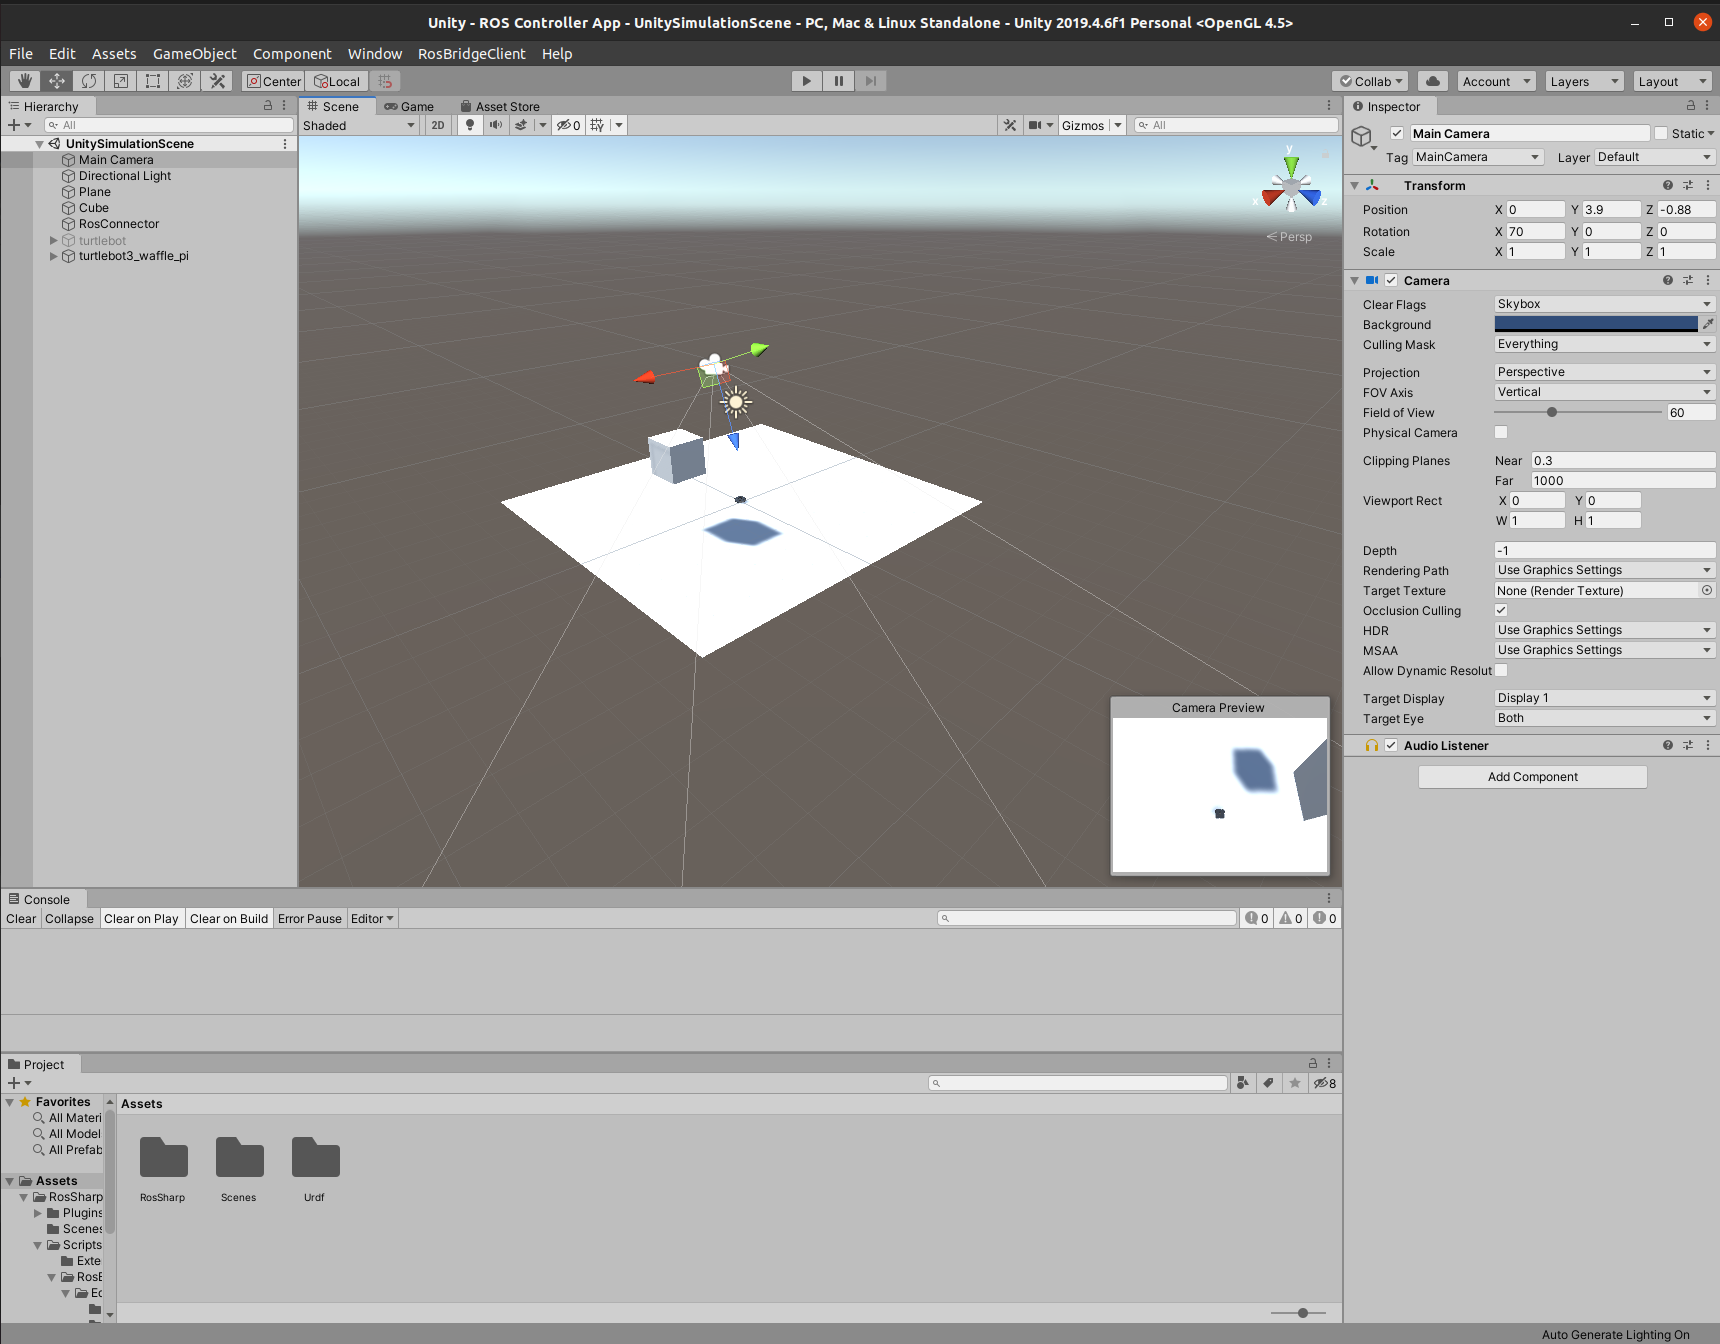
\includegraphics[height=12cm,width=21cm,keepaspectratio=true]{unitySS}
		\caption{Unity Editor}
		\label{fig:unityeditor}
	\end{center}
\end{figure}
\newpage

\subsection{Skripte}

\qquad Unity tako�er svojim korisnicima omogu�ava programiranje vlastitih (ili kori�tenje tu�ih) skripta. Programiranje se vr�i u C\# programskom jeziku, koji se izvr�ava na \textit{Mono} razvojnom okru�enju. Tako�er, mogu�e je skripte programirati u \textit{JavaScriptu}, ali je podr�ka lo�ija.

\qquad Cilj \textit{Mono} razvojnog okru�enja je da omogu�i kori�tenje .NET Framework-a na razne operacijske sustave, jer je ina�e .NET framework razvijen od strane Microsofta samo za Windows OS. Komponente \textit{Mono} framework-a uklju�uju:
\begin{itemize}
	\item C\# kompajler - Potpun kompajler, sa svim zna�ajkama od C\# 1.0 do 6.0.
	\item Mono Runtime \cite{monoabout} - Glavne komponente:
	\begin{itemize}
		\item Just-in-Time (JIT) kompajler - kompilacija koda tokom izvr�avanja programa. 
		\item Ahead-of-Time (AOT) kompajler - kompilacija koda u nativni kod stroja gdje �e se izvr�avati, prije njegovog izvr�avanja.
		\item �ita� knji�nica - omogu�uje nam u�itavanje vanjskih programskih knji�nica.
		\item Sakuplja� sme�a (Garbage collector) - automatsko brisanje objekata u memoriji koji se vi�e ne koriste.
		\item Dretveni sustav - omogu�ava izvr�avanje vi�e dretva (threads) istovremeno, pospje�uje brzinu i produktivnost odre�enog programa ako je isprogramirano na pametan na�in.
		\item Interoperabilnost - karakteristika da vi�e programskih sustava mogu bez pote�ko�a me�usobno funkcionirati.
	\end{itemize}

	\item .NET Framework knji�nica klasa - \textit{Mono} platforma pru�a set klasa kao temelj za razvijanje aplikacija. Navedene su klase kompatibilne s Microsoftovim .NET Framework klasama.
	\item \textit{Mono} pru�a i dodatne klase koje nisu uklju�ene u Microsoftovim baznim klasama koje su posebice korisne za razvijanje Linux aplikacija, npr. Gtk+, Zip, OpenGL, Cairo, POSIX i druge.
\end{itemize}
\qquad Glavne zna�ajke \textit{Mono} radnog okru�enja:
\begin{itemize}
	\item Multi-platformsko radno okru�enje - Linux, macOS, BSD, Microsoft Windows.
	\item Multi-jezi�an - C\#, VB 8, Java, Python, Ruby i jo� mnogi.
	\item Kompatibilan s binarnim kodom.
	\item Kompatibilan s Microsoft APIjem - pokre�e ASP.NET, ADO.NET, Silverlight i Windows.Forms.
	\item Otvorenog koda i besplatan - sav \textit{Mono} sadr�aj, uklju�uju�i i knji�nice, distribuiran je koriste�i MIT licencu.
	\item Opse�na pokrivenost - implementacije mnogih popularnih knji�nica i protokola.
\end{itemize}

\qquad Programiranje prilago�enih skripti omogu�ava kompleksna pona�anja i radnje u igri/softveru kojega se razvija. Gotovo sve akcije koje se mo�e napraviti u Editoru, mo�e se i u skripti, te se time mo�e drasti�no pove�ati opseg mogu�nosti.
\clearpage

\section{ROS\#}
\qquad ROS\# je set programskih knji�nica i alata otvorenog koda u C\#-u koja omogu�uje komunikaciju izme�u ROS-a i .NET aplikacija - Unity-ja, razvijen od strane Siemens kompanije. ROS\# je bio primarno razvijen za Windows OS, ali se uspje�no mo�e koristiti i na druge operacijske sustave. Paket se mo�e preuzeti s Unity Asset Store-a ili direktno sa slu�benog Github repozitorija. \cite{rossharprepo} Ovo je ujedno i glavni alat koji �e se koristiti u ovom radu za stvaranje mosta izme�u ROS-a i Unity-a.

\qquad Glavni sadr�aj ovog paketa je sljede�i:
\begin{itemize}
	\item .NET rje�enje za RosBridgeClient (knji�nica koja omogu�uje spajanje vanjskih aplikacija na ROS sustav), Urdf (robotski modeli) i MessageGeneration (generiranje poruka).
	\item ROS paketi kori�teni od strane ROS\#-a.
	\item Unity projekt koji sadr�i primjer scenu te RosBridgeClient, Urdf i MessageGeneration ekstenzije za Unity.
\end{itemize}

\subsection{RosBridgeClient}

\qquad RosBridgeClient za spajanje .NET baziranih aplikacija na ROS koristi \emph{rosbridge\_suite}. \emph{rosbridge\_suite} pru�a ROS-u API funkcionalnost za programe koji su izvan ROS sustava. Isti koristi naredbe bazirane na JSON formatu. Transportni sloj je implementiran u \emph{rosbridge\_server} paketu koji pru�a WebSocket poveznicu. \cite{rosbridgesuite} WebSocket je konstantna poveznica izme�u klijenta i servera gdje se promet odvija u oba smjera te koristi TCP/IP protokol.

 
% !TeX encoding = windows-1250
\chapter{Opis rje�enja}

\qquad Nastavno na dosad navedeno opisat �e se aplikacija i njezina struktura, kako je ista napravljena i na kojem principu funkcionira. Tri glavne komponente ovog sustava, kao �to je ve� navedeno, su: ROS, ROS\# i Unity. Na slici \ref{fig:maindiagram} prikazan je dijagram kako sustav izgleda gdje su nam navedene komponente i glavni dijelovi sustava.

\qquad Prvi korak sustava jest pokretanje Gazebo simulacije u ROSu gdje se simulira robota i njegovo okru�enje. Alternativa u pravom svijetu bi bila ista osim �to ne bismo trebali pokretati Gazebo ve� pravog robota na kojemu se tako�er izvr�ava ROS.

\qquad Drugi korak jest Unity odnosno Editor i njegove standalone te mobilne aplikacije koje su implementirane i adaptirane sa istom svrhom i mogu�nostima. �to zna�i da se mo�e bilo koja aplikacija pokrenuti i spojiti na navedeni robotski sustav.

\qquad ROS\# paket, odnosno most koji spaja ROS i Unity pomo�u RosBridgeClient-a otvara vezu izme�u prethodno navedena dva koraka, a koji funkcionira na temelju pretplate i izdavanja poruka na ROS teme (eng. topic). Jednom kad se veza otvorila, Unity se mo�e pretpla�ivati na ROS teme i izdavati nove poruke na ROS teme.

\qquad Na slici \ref{fig:maindiagram} prikazan je glavni princip prethodno navedenih mogu�nosti:
\begin{enumerate}
	\item Unity se pretpla�uje na ROS teme - povratne informacije, npr. odometrija, slika kamere, laserski sken.
	\item Unity izdaje nove poruke na ROS teme - kontrolne poruke, npr. upravljanje robotom.	
\end{enumerate}

\begin{figure}[!htbp]
	\begin{center}
		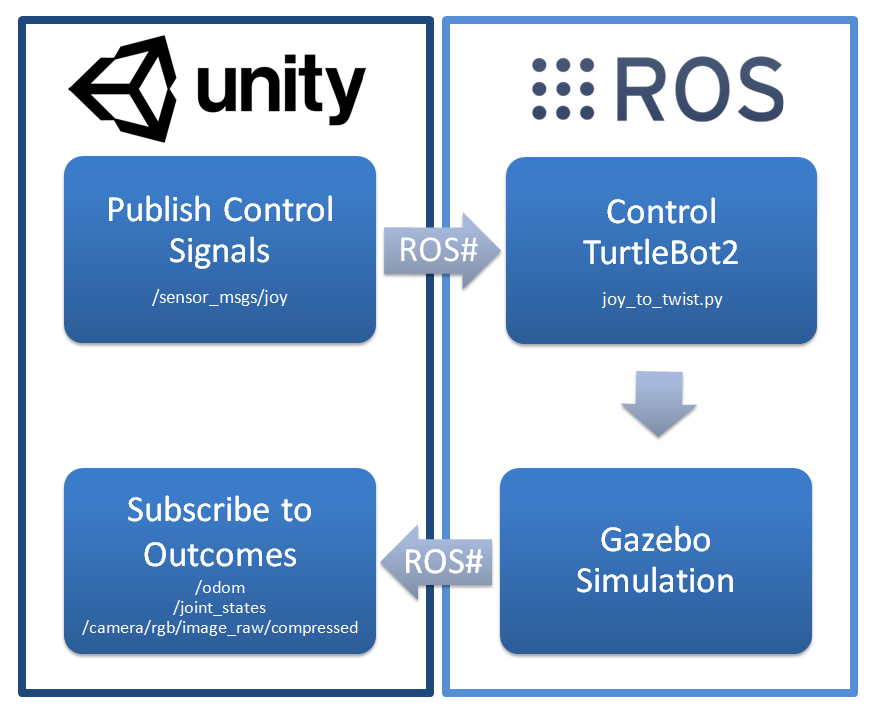
\includegraphics[height=12cm,width=21cm,keepaspectratio=true]{diagram}
		\caption{Dijagram sustava \cite{rossharpgazebosim}}
		\label{fig:maindiagram}
	\end{center}
\end{figure}
\clearpage

\section{Opis su�elja i Unity objekata}

\qquad U ovoj �e se sekciji opisati koji su i �emu slu�e glavni objekti u kori�tenim Unity scenama.

\subsection{Meni}
\qquad Napravljen je jednostavni inicijalni meni s nekoliko polja za upis:
\begin{enumerate}
	\item IP adresa - polje za unos IP adrese ROS-a, tj. robota. IP adresu, ako je nepromjenjiva, dovoljno je upisati jednom jer se sprema pomo�u Unity zna�ajke \emph{PlayerPrefs} koja slu�i za spremanje igra�evih (korisni�kih) postavka.
	\item Prefiks robota - opcionalno polje u slu�aju da postoji vi�e robota u simulaciji. 
\end{enumerate}

Postoje i dva gumba gdje svaki vodi na jednu scenu gdje je implementirana neka zna�ajka. Na svakoj od ovih scena se vr�i spajanje na ROS i zapo�inje interakcija:
\begin{enumerate}
	\item Gumb koji vodi na scenu (dalje u tekstu scena 1) gdje je implementirana kontrola robota, pogled u prvom licu s kamere, 2D mapiranje i prikaz podataka laserskog skena.
	\item Gumb koji vodi na scenu (dalje u tekstu scena 2) gdje se vr�i 3D mapiranje prostora.
\end{enumerate}

Sljede�e �e se navesti svi elementi (objekti) u sceni 1 te �emu slu�e.

\subsection{Ros Connector}

\qquad Na sceni 1 najbitniji element, tj. objekt, jest \textbf{RosConnector} koji prvobitno slu�i za otvaranje veze prema ROS-u, ali i za sadr�avanje svih skripta kojima je zada�a pretplata ili izdavanje poruka na ROS temu. \textbf{RosConnector} sadr�i sljede�e relevantne skripte:
\begin{enumerate}
	\item \emph{Image Subscriber} koji se pretpla�uje na jednu ROS temu kamere, u ovom slu�aju se koristi \emph{/camera/rgb/image\_raw/compressed}.
	\item \emph{Laser Scan Subscriber} koji se pretpla�uje na ROS temu laserskog skena (\emph{/scan}). 
	\item \emph{Map Subscriber} koji se pretpla�uje na ROS temu \emph{/map} koju izdaje �vor \emph{slam\_gmapping}. 
	\item \emph{Odometry Subscriber} koji se pretpla�uje na temu \emph{/odom} i dohva�a odometrijske podatke robota.
	\item \emph{Joystick Publisher} izdaje poruke na \emph{/joy} ROS temu, koja slu�i kao joystick kontrola robota.
	\item \emph{Twist Publisher Static} u�itava ulaz gumbova na glavnoj sceni za upravljanje smjerom robota. Isti izdaje poruke na \emph{/cmd\_vel} ROS temi koja upravlja linearnom i kutnom brzinom robota.
\end{enumerate}

\subsection{Plane}

\qquad Plane je 3D objekt koji slu�i kao podloga (pod ili teren) robotu. Bez podloge bi se trebalo isklju�iti svojstvo gravitacije u Unityju, no na taj na�in se mo�e podloga iskoristiti za projekciju generirane 2D mape okoline robota. Na na�in kada stavimo prikaz scene iznad navedenog objekta i robota, dobiva se efekt robota koji ide kroz mapu koja se paralelno izra�uje.

\subsection{Model robota}

\qquad Model robota se prikazuje kao zaseban objekt u sceni, u ovom slu�aju objekt \textbf{turtlebot3\_waffle\_pi}. Isti je generiran prija�nje navedenim alatom za uvoz URDF modela i sadr�i podobjekte po svojstvima robota kao na slici \ref{fig:robotmodel}.

\begin{figure}[!htbp]
	\begin{center}
		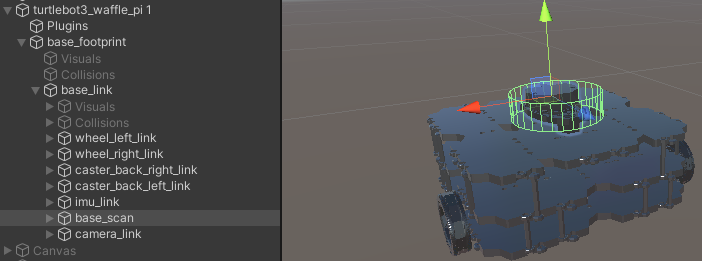
\includegraphics[height=8cm,width=14cm,keepaspectratio=true]{robotModel}
		\caption{Model robota u Unity-ju}
		\label{fig:robotmodel}
	\end{center}
\end{figure}

Pomi�ni podobjekti, npr. kota�i, se vrte isto kao i u simulaciji zahvaljuju�i pomo�nim skriptama ROS\#a koje u�itavaju stanja kota�a sa simulacije. 

\subsection{Canvas}

\qquad \textbf{Canvas} u Unityju je 2D objekt koji ve�inom slu�i za slaganje grafi�kih komponenta su�elja, npr. gumbovi, tekst ulazi i sl. Jedna od najve�ih prednosti Canvasa je responzivnost. Canvas-u se mo�e definirati bazna rezolucija, koja se onda mo�e skalirati ovisno o rezoluciji ure�aja gdje je aplikacija pokrenuta. Isto vrijedi za sve elemente u Canvasu. Elementi se mogu "usidriti" u nekom kutu ekrana, mogu se �iriti i smanjivati ovisno o rezoluciji, mijenjati poziciju ovisno o veli�ini ekrana i sl.

U ovoj aplikaciji Canvas se sastoji od sljede�ih elemenata:
\begin{enumerate}
	\item \emph{Camera Image} kao �to ime govori, je element Canvasa gdje nam se prikazuje slika s kamere. Slika kamere u�itava se kao tekstura te se ista preslikava kao \emph{Sprite} (grafi�ki element u Unityju - slika) na navedeni element koji sadr�i polje za sliku. Element je pro�iren po cijeloj du�ini i �irini Canvasa, tako da se ovisno o rezoluciji ekrana skalira.
	\item \emph{Control} je objekt koji sadr�i podobjekte koji su gumbovi za odre�ivanje linearne i kutne brzine robota. 
	\item \emph{Laserscan Button} je gumb koji uklju�uje i isklju�uje prikaz objekata generiranih laserskim skenom.
	\item \emph{Camera Button} je gumb koji mjenja prikaz kamere (topografski prikaz mape i robota te prikaz u prvom licu s kamere robota).
	\item \emph{2D Map Button} je gumb koji uklju�uje i isklju�uje crtanje i prikaz 2D mape na \emph{Plane} objekt.
	\item \emph{Switch Robot Camera} mjenja prikaz kamere u prvom licu na drugog robota (u slu�aju da ima vi�e robota u simulaciji). Ako u simulaciji postoji samo jedan robot, tada je taj gumb isklju�en.
	\item \emph{FPS} koji prikazuje trenutni FPS (broj a�uriranja slike u sekundi) u sceni.
\end{enumerate}

\subsection{Multi Robot Control}

\qquad \emph{Multi Robot Control} objekt slu�i samo za pokretanje skripte koja omogu�uje prikaz kamera dva robota odjednom.
\clearpage

\subsection{Scena 2}

\qquad Scena 2 sadr�i iste elemente kao scena 1 osim �to od Canvas gumbova ima samo \emph{Control}, \emph{FPS} i novi \emph{3D Map Button} koji slu�i za aktiviranje i deaktiviranje crtanja 3D objekata u sceni - 3D mape.

\section{Zna�ajke i mogu�nosti rje�enja}

\qquad U sljede�oj �e se sekciji navesti i opisati zna�ajke i mogu�nosti koje se implementiralo u ovom radu.

\subsection{Kamere}

\qquad U sceni postoje dvije kamere. Kamera u Unityju ozna�ava kako se scena prikazuje. Ona mo�e biti iz razli�itih kuteva, sa razli�itom �irinom i dubinom snimanja, bilo kojom pozicijom snimanja i jo� mnogo postavka. Jedna �e kamera biti postavljena iznad 3D objekata, a druga �e biti namje�tena da snima Canvas - u ovom slu�aju pozicija kamere nije bitna jer fiksno snima 2D Canvas.

Prikaz kamere iz prvog lica - Prva zna�ajka na koju se nailazi prilikom pokretanja aplikacije je prikaz kamere iz prvog lica. Slika se u stvarnom vremenu dohva�a sa robota te se kao tekstura postavlja na prija�nje navedenom Canvas objektu.

Prikaz kamere iz pti�je perspektive - U ovoj se perspektivi prikazuje 3D model robota na 2D mapi koja se izra�uje s dobivenim podacima iz \emph{/map} ROS teme, gdje se izra�uje nova tekstura koja se precrtava na \emph{Plane} objekt. U ovoj su perspektivi tako�er vidljive sfere (tako�er 3D objekti) koji se crtaju shodno podacima iz \emph{/scan} ROS teme (laserskog skena).


\subsection{Laserski sken}

\qquad ROS teme laserskog skena �alju poruke formata \emph{sensor\_msgs/LaserScan} u kojem se nalazi vi�e vrsta podataka, ali je u ovom slu�aju bitno float32 polje \emph{ranges}. Problem je �to ovo polje zna sadr�avati beskona�ne brojeve te tada ROS\# izbacuje gre�ku i ne nastavlja s procesiranjem tog polja. Iz tog razloga bilo je potrebno napraviti ROS �vor koji �e �itati temu laserskog skena, ROS tema \emph{/scan}, filtrirati podatke koji su beskona�ni te izdati novu ROS temu sa ispravljenim podacima. Dobiveni podaci se pomo�u ROS\# skripte \emph{Laser Scan Writer} i \emph{Laser Scan Visualizer} crtaju kao sfere u 3D prostoru oko robota. 

\subsection{2D mapiranje}

\qquad 2D mapiranje u Unityju se vr�i na na�in da se u�itavaju podaci iz ROS tema \emph{/map}. Ista �alje poruke tipa \emph{nav\_msgs/OccupancyGrid}. Najrelevantniji podaci ove teme su nam �irina i du�ina mape te int8 polje podataka u kojem se nalaze podaci vjerojatnosti u rasponu od 0 do 100 - vjerojatnost da je jedno skenirano polje zauzeto nekim objektom u prostoru. Kada se vjerojatnost ne mo�e izra�unati, u polju podataka bude broj -1.
Proces crtanja mape u Unityju je sljede�i:
\begin{enumerate}
	\item U�itava se du�ina i �irina mape.
	\item Inicijalizira se nova varijabla za mapu koja �e biti tipa \emph{Color} i biti �e iste duljine kao i polje podataka iz \emph{/map} teme.
	\item Iterira se po tom dobivenom polju podataka te se ovisno o dobivenom podatku u novoinicijalizirano polje boja dodaje nova definirana boja.
	\item Nakon iteriranja je potrebno postaviti zastavicu (flag) u \emph{true} koja predstavlja da je potrebno nacrtati novu mapu na su�elju.
	\item Unity funkcija \emph{Update()} koja se izvr�ava svako osvje�avanje ekrana, provjerava navedenu zastavicu i izra�uje novu teksturu na temelju definiranog polja boja, du�ine i �irine mape te se nova tekstura sprema na glavnu teksturu \emph{Renderer} komponente na \emph{Plane} objektu. 
\end{enumerate}

Kori�tena metoda mapiranja je \emph{SLAM (Simultana Lokalizacija i Mapiranje) gmapping} koja je bazirana na podacima laserskog skena i pozicije robota. Ista je stvoritelj prija�nje navedenih \emph{Occupancy Grid} podataka (mre�a popunjenosti) tj. mape. Mapa se a�urira u intervalu od 4 sekunde.

Ispunjavanje novog polja boja u petlji je vrlo ne optimiziran pristup. U aplikaciji se osje�ao trzaj u izvr�avanju tijekom izrade mape, pa se kao rje�enje na to izvr�avanje funkcije koja sadr�i petlju izvr�ava kao novi \emph{Task} koji u C\# ozna�uje asinkronu operaciju na novoj dretvi. Time se drasti�no smanjio trzaj u aplikaciji.

\subsection{Upravljanje}

\qquad Upravljanje robotom se mo�e vr�iti na dva na�ina: 
\begin{itemize}
	\item Kori�tenjem gumbova na su�elju - Svaki gumb inkrementira ili dekrementira brzinu za definirani korak. Trenutno definirani korak za linearnu brzinu iznosi 0.05, a za kutnu 0.02. Svakom promjenom se na \emph{/cmd\_vel} ROS temi �alje poruka tipa \emph{geometry\_msgs/Twist} s novom brzinom. Poruka sadr�i Vector3 tip varijable za linearnu i kutnu brzinu. \emph{/cmd\_vel} ROS tema proslije�uje naredbe brzine samom robotu.
	\item Kombinacijom tipka (w, a, s, d) ili tipka strelica - Unity pomo�u ROS\# pomo�nih skripti koje u�itavaju promjenu u ulazu \emph{Input Managera}, pretvara ulaze u upravlja�ku naredbu za \emph{/joy} ROS temu. Nakon toga ROS\# �vor \emph{joy\_to\_twist} pretvara poruke \emph{/joy} ROS teme u poruke formata \emph{geometry\_msgs/Twist} te �alje na ROS temu \emph{/cmd\_vel}. Unity \emph{Input Manager} je dio postavka gdje se mogu konfigurirati na�ini ulaza naredba u aplikaciju.
\end{itemize}

Samo se jedna od navedenih metoda mo�e koristiti odjednom iz razloga �to obe metode �alju poruke na istu ROS temu (\emph{/cmd\_vel}) pa �e u slu�aju kori�tenja obe metode, metoda joysticka ili tipka premostiti metodu gumbova. 

Povratna informacija s \emph{/odom} ROS teme se koristi za a�uriranje odometrijskih podataka robotskog modela u Unity prostoru.

\subsection{Prikaz s vi�e robota}

\qquad U svrhu istra�ivanja, omogu�eno je da se mogu prikazivati slike kamera u simulaciji gdje postoje dva robota iste vrste. Kao primjer je uzeta i adaptirana Turtlebot 3 simulacija s vi�e robota.

U po�etnom izborniku potrebno je upisati prefiks ROS tema ispred teme robota, npr. postoji simulacija s vi�e Turtlebotova gdje svaki Turtlebot ima svoje ROS teme koje su ina�e istog naziva, njima je potrebno dodati prefiks ispred naziva ROS teme da bi se znalo na kojeg Turtlebota se ta ROS tema odnosi (slika \ref{fig:multirobotexample}). Prefiks je potrebno definirati u glavnoj \emph{launch} datoteci simulacije kao �to je u sljede�em isje�ku XML koda gdje je prefiks string \emph{tb} u \emph{default} svojstvu argumenata. \\

\begin{lstlisting}
<launch>
	<arg name="model" default="$(env TURTLEBOT3_MODEL)" doc="model type [burger, waffle, waffle_pi]"/>
	<arg name="first_tb3"  default="tb1"/>
	<arg name="second_tb3" default="tb2"/>
</launch>
\end{lstlisting}

Ova je funkcija napravljena na na�in da u sceni postoji dodatni neaktivni \emph{RosConnector} i model robota, koji se ovisno o ulazu na glavnom izborniku uklju�uje. Pri pretpla�ivanju pojedina�nog robota na ROS teme, u glavnoj se ROS\# \emph{Unity Subscriber} skripti provjerava broj robota te se u ovom slu�aju dodaje spomenuti prefiks u ROS temu. Promjena robota (kamere) se vr�i na na�in da se uklju�uje kamera jednog robota a isklju�uje kamera drugog robota a obe kamere su namje�tene kao glavni prikaz.

Pri pokretanju i spajanju na simulaciju, prija�nje navedenim gumbom mogu�e je mijenjati pogled s jednog robota na drugi. U ovoj se simulaciji roboti kre�u sami te su ostale funkcije onemogu�ene.

\begin{figure}[!htbp]
	\begin{center}
		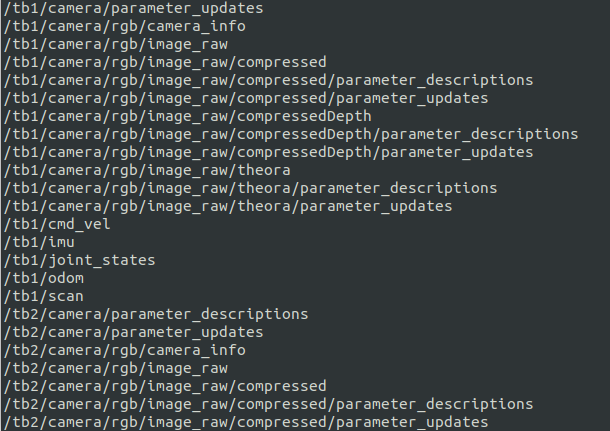
\includegraphics[height=8cm,width=16cm,keepaspectratio=true]{multiRobotExample}
		\caption{Primjer ROS tema s vi�e robota}
		\label{fig:multirobotexample}
	\end{center}
\end{figure}

\clearpage

\subsection{3D mapiranje}

\qquad Za izradu podataka 3D mape kori�ten je \emph{octomap\_mapping} koji izra�uje 3D mre�u popunjenosti (eng. 3D occupancy grid). Navedena metoda se koristi pokretaju�i \emph{octomap\_server} �vor koji omogu�ava inkrementalno izgra�ivanje i spremanje mape te distribuira mapu ostalim �vorovima preko svojih ROS tema. \cite{octomap}

\qquad Analizom dostupnih \emph{octomap} �vorova odlu�eno je da bi najprikladniji �vor za Unity bio \emph{/octomap\_point\_cloud\_centers} koji �alje poruke formata \emph{sensor\_msgs/PointCloud2}. PointCloud2 je prikladan format za Unity iz razloga �to sadr�i kolekciju N-dimenzionalnih to�aka, u tom slu�aju 3 dimenzije (x, y, z). Navedeni �vor objavljuje to�ke u stvorenoj 3D mapi napravljenoj od strane \emph{octomap} alata. Naime, odabrani �vor je potrebno procesirati da bi se iz njega dobilo x, y, z to�ke. U tom cilju potrebno je napraviti dodatni �vor koji se pretpla�uje na odabrani �vor, procesira podatke te ih procesirane objavljuje u novi �vor na kojega �e se Unity pretpla�ivati. Za procesiranje podataka kori�tena je gotova funkcija za tu svrhu iz \emph{ros\_numpy} knji�nice koja adaptira poznati Pythonov \emph{numpy} za ROS, \emph{point\_cloud2.pointcloud2\_to\_array}. Dobiveno polje podataka nije mogu�e objaviti bez da postoji ROS poruka tog formata. U tu svrhu napravljene su dvije nove ROS poruke, \emph{CustomPointCloud} i \emph{CustomPointCloudMsg}.

\emph{CustomPointCloud} sadr�i to�ke (x, y, z) u float32 formatu dok \emph{CustomPointCloudMsg} sadr�i polje \emph{CustomPointCloud} poruka. Kombiniranjem dvije poruke jedini je na�in za napraviti intuitivni format podataka za lak�e naknadno procesiranje u Unityju.

Imaju�i na raspolaganju prilago�ene ROS poruke za potrebe ovog rada sada je mogu�e u prija�nje navedenom novom �voru napraviti novu poruku formata \emph{CustomPointCloudMsg} u kojem �e se spremiti sve to�ke u 3-dimenzionalnom prostoru te objavljivati na novi �vor \emph{/octomap\_point\_cloud\_centers\_filtered}.

Sljede�e je potrebno izmijeniti ROS\# knji�nicu, tj. dodati nove ROS poruke jer ina�e Unity nebi mogao primati poruke stvorenog �vora. U ROS\# .NET projekt dodaju se dvije nove klase u mapu \emph{MessageTypes} koje implementiraju isti format podataka kao stvorene ROS poruke. Projekt treba ponovno izgraditi te izmijenjene .dll datoteke dodati u Unity projekt.

U aplikaciji se vr�i klasi�nu pretplatu na novi �vor \emph{/octomap\_point\_cloud\_centers\_filtered} te dobivene poruke spremamo u novostvoreni format. Stvaranje i prikaz 3D mape se vr�i na sljede�i na�in:

\begin{enumerate}
	\item Pri primitku nove poruke, pokre�e se funkcija za stvaranje objekata u sceni koji �e reprezentirati dobivene to�ke 3D mape.
	\item Petljom prolazimo kroz sve dobivene to�ke. Za svaku to�ku stvara se kocku kojoj se dodijeljuje veli�ina i (x, y, z) pozicija u Unity prostoru.
	\item Primitkom nove poruke, ponovno se pokre�e funkcija za stvaranje objekata (a�uriranje mape) samo ako je prija�nje pozivanje funkcije gotovo.
\end{enumerate}
Ovim koracima stvara se 3D mapa u Unity aplikaciji.

\subsection{RQT graf sustava}

\qquad Na slici \ref{fig:rqtgraph} prikazan je cjelovit RQT graf sustava. \emph{rqt\_graph} je grafi�ki alat za prikaz ROS grafa pokrenutog sustava/aplikacije. U njemu su prikazane poveznice izme�u pokrenutih ROS tema i �vorova.

U grafu je vidljivo da sve ROS teme s povratnim informacijama idu u \emph{/ros\_websocket} a iz njega odlaze poruke u ROS teme za upravljanje robotom.

\begin{figure}[!htbp]
	\begin{center}
		\includegraphics[height=8cm,width=16cm,keepaspectratio=true]{rqtGraph}
		\caption{RQT graf sustava}
		\label{fig:rqtgraph}
	\end{center}
\end{figure}

 
% !TeX encoding = windows-1250
\chapter{Rezultati}

\section{Aplikacija}

\qquad Uspje�no su napravljene funkcionalne aplikacije za sve �eljene platforme (Windows, Linux i Android). Razvijanje sveukupnog sustava vr�ilo se na Linux Ubuntu operacijskom sustavu, a za ostale platforme napravilo se samo potrebne promjene, izgra�ivanje i testiranje aplikacije. Na slici \ref{fig:winunity} prikazana je aplikacija u Unity Editor-u.

\begin{figure}[!htbp]
	\begin{center}
		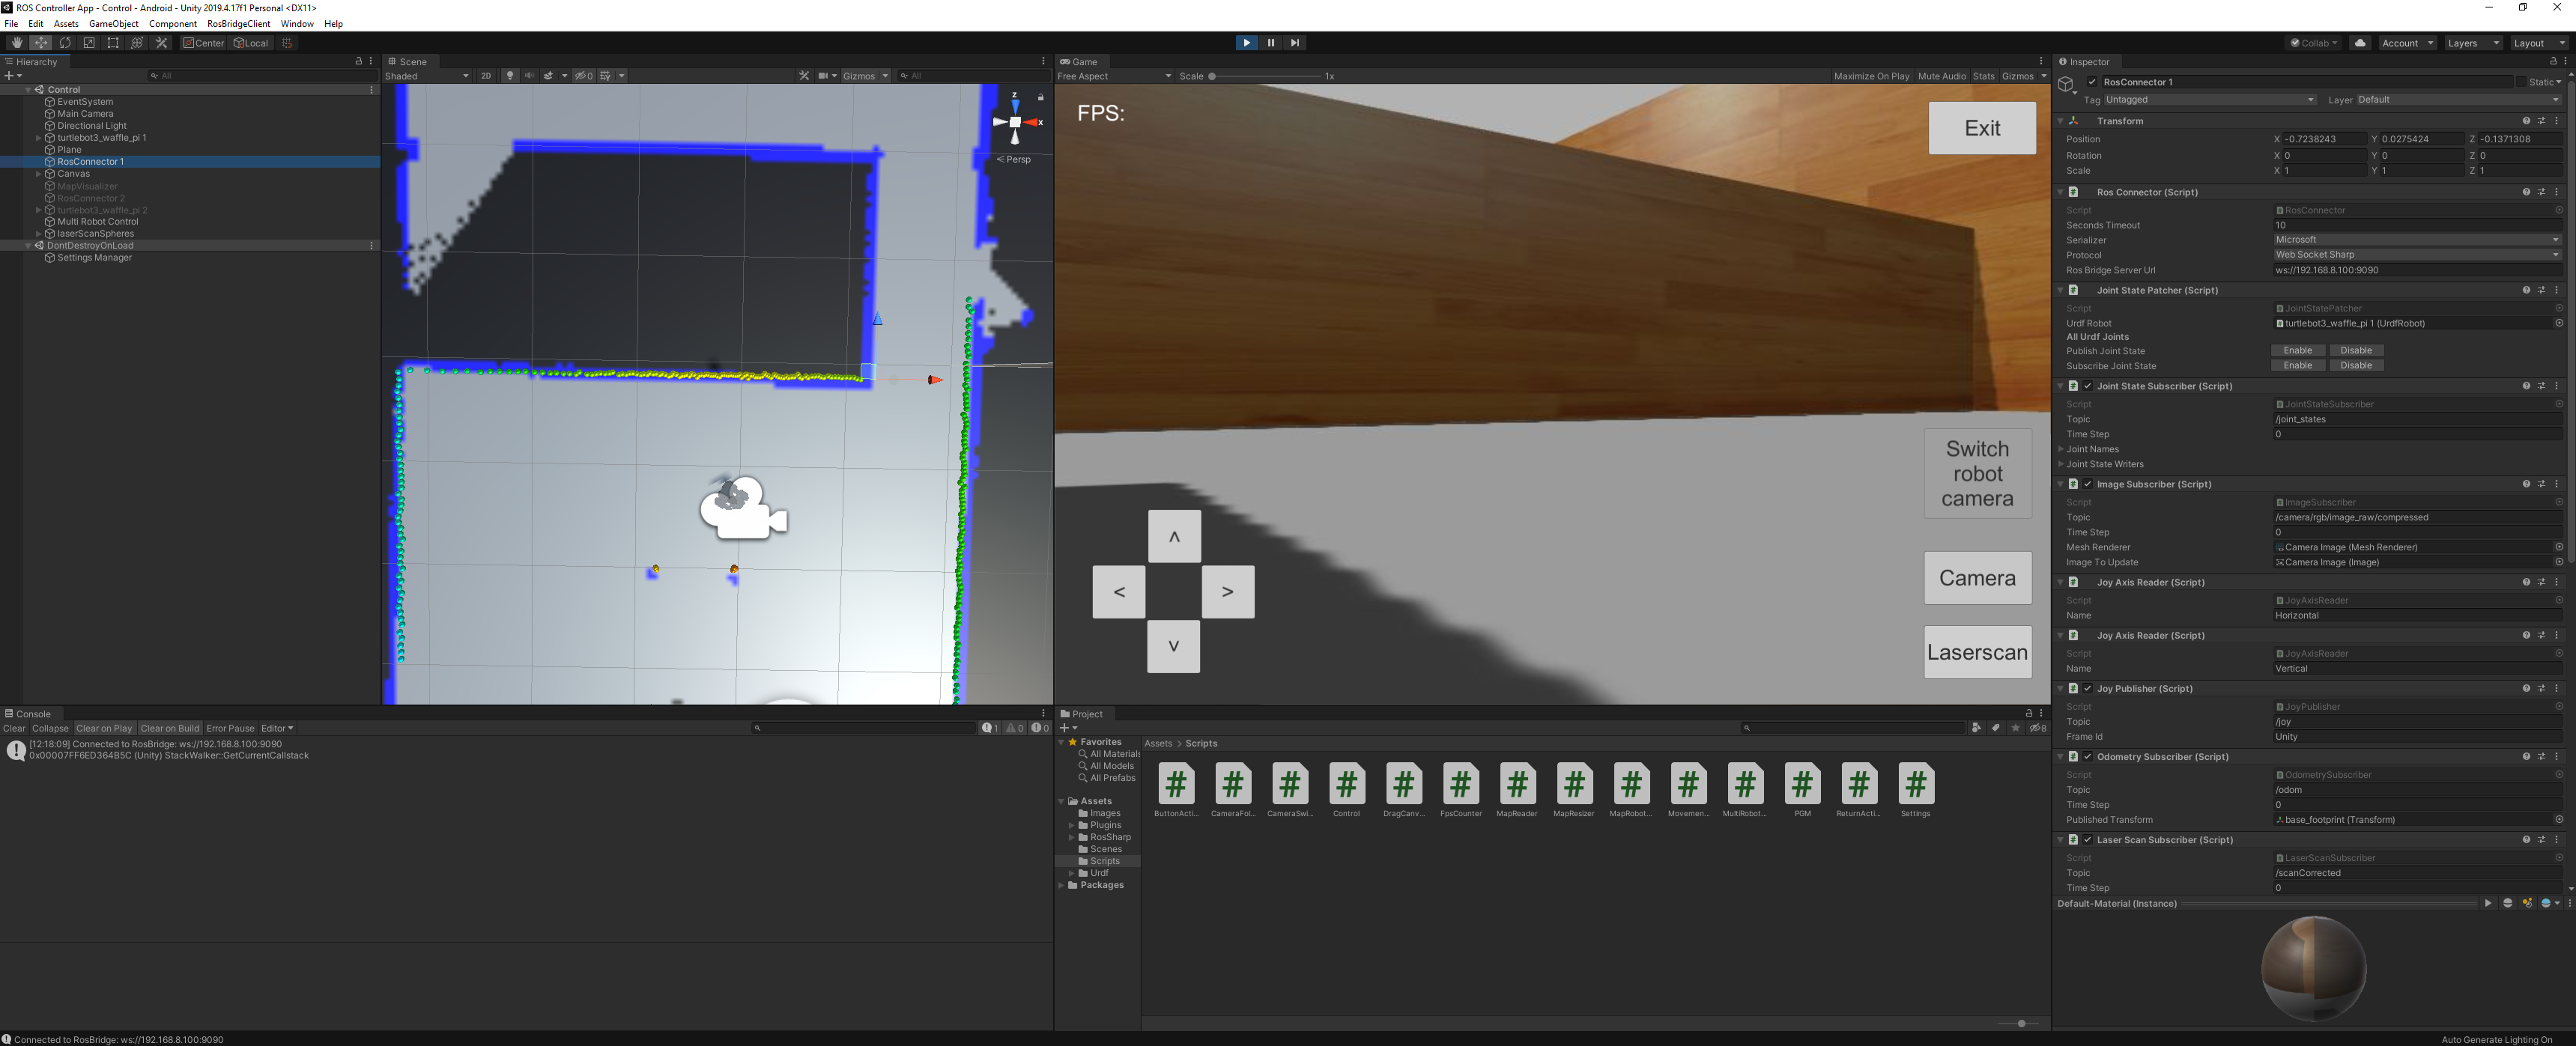
\includegraphics[height=12cm,width=16cm,keepaspectratio=true]{winUnity}
		\caption{Aplikacija u Unity Editor-u}
		\label{fig:winunity}
	\end{center}
\end{figure}

Unity podr�ava WebGL, pa je i to poku�ano napraviti, ali neuspje�no. Pretpostavka ovog neuspjeha le�i u tome �to Unity WebGL koristi \emph{WebAssembly} tehnologiju, koja ne podr�ava uvijek sve module koje se �eli koristiti. \emph{WebAssembly} je noviji tip koda koji se mo�e izvr�avati na modernim web preglednicima. Isti je low-level programski jezik sli�an \emph{asembleru} u binarnom formatu koji se izvr�ava sa sli�nim performansama kao u nativnoj aplikaciji. On omogu�uje aplikacije koje su napisanu u C-u, C++-u, C\#-u i Rust-u da se prekompajlaju i omogu�i im se izvr�avanje na web-u \cite{webassembly}.

\subsection{Linux i Windows}

\qquad Linux i Windows desktop aplikacije su po izgledu iste, ali se razlikuju u performansama. Windows se pokazao najlo�iji u izvedbi aplikacije, unato� puno superiornijim hardverom. Linux Ubuntu u drugu ruku, unato� �to se na njemu izvr�avala i simulacija, performanse nisu padale. U tablici \ref{tab:pchardver} vidljive su razlike u hardveru, gdje su Windows komponente, komponente stolnog ra�unala pa su puno mo�nije te rade na vi�oj frekvenciji.

\begin{table}[!htbp]
	\scriptsize
	\renewcommand{\arraystretch}{1.2}
	\caption{Windows i Linux hardver ra�unala}
	\centering
	\begin{tabular}{|c|c|c|}
		\hline
		Komponenta & Windows & Linux Ubuntu (prijenosno ra�unalo)
		\\ [0.5ex]
		\hline \hline
		CPU & Intel Core i7-10700 (8 jezgri, 16 dretvi) & Intel Core i7-9750H (6 jezgri, 12 dretvi) \\ [0.5ex] 
		GPU & NVIDIA GeForce GTX 1660 6GB Super & NVIDIA GeForce RTX 2060 6GB mobile \\ [0.5ex]
		RAM & 16GB XMP & 16GB \\ [0.5ex]
		\hline
	\end{tabular}
	\label{tab:pchardver}
\end{table}

Na slici \ref{fig:laserscan} prikazan je pogled iznad objekata u sceni gdje obojane sfere prikazuju podatke laserskog skena kojima je intenzitet boje sve ja�i �to je robot bli�e predmetu u prostoru, dok je podloga ispod robota i sfera generirana mapa. Slika \ref{fig:win2} prikazuje pogled iz kamere robota - u ovom na�inu rada aplikacija bude najfluidnija zbog konstantnog dotoka informacija (slike) koja zahtjeva minimalno dodatno procesiranje sa strane aplikacije.

\newpage

\begin{figure}[!htbp]
	\begin{center}
		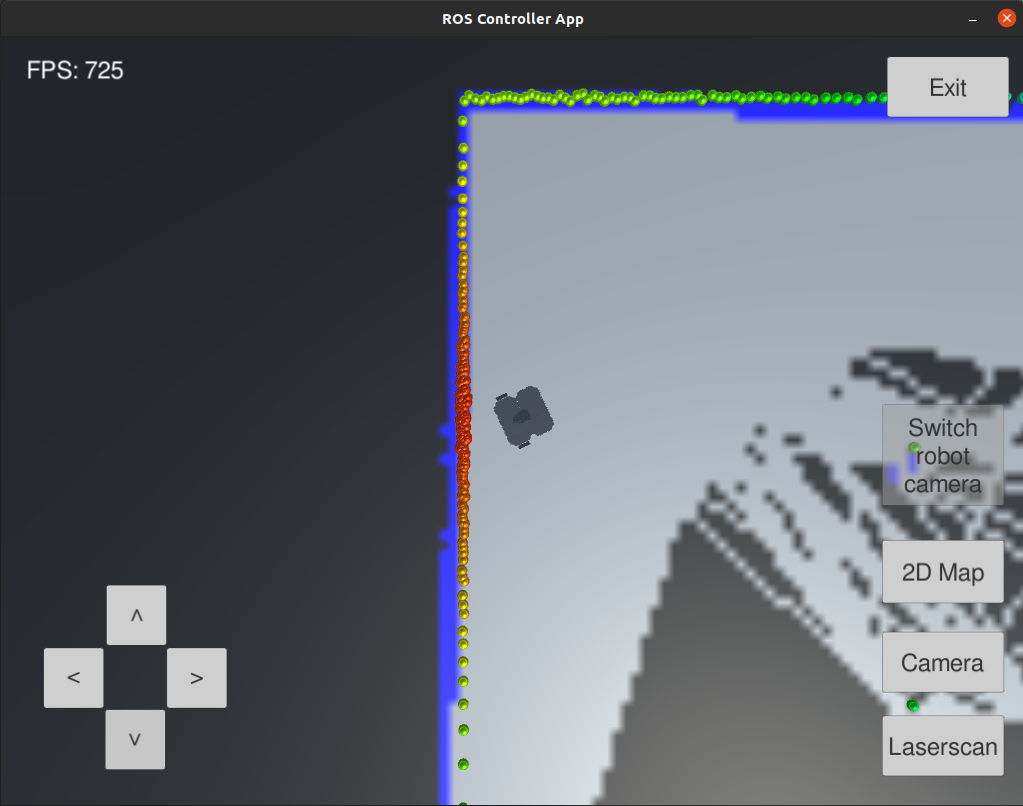
\includegraphics[height=10cm,width=10cm,keepaspectratio=true]{laserscan}
		\caption{Linux aplikacija - mapa, robot i laserski sken}
		\label{fig:laserscan}
	\end{center}
\end{figure}

\begin{figure}[!htbp]
	\begin{center}
		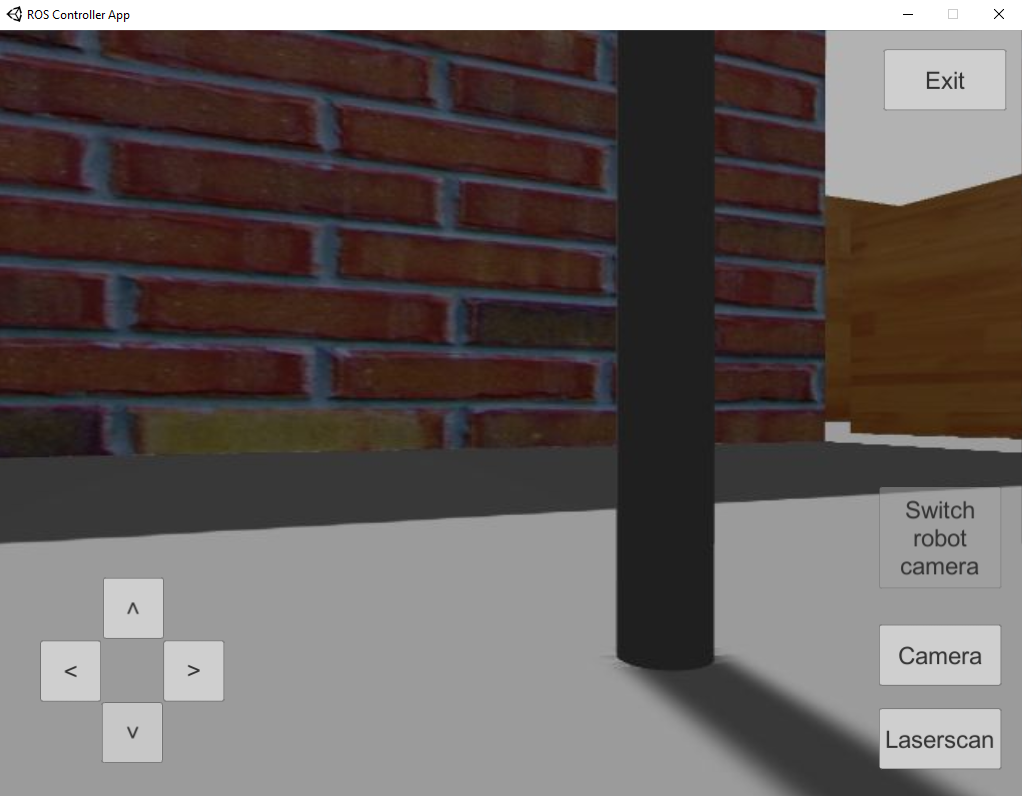
\includegraphics[height=10cm,width=10cm,keepaspectratio=true]{win2}
		\caption{Windows aplikacija - pogled iz kamere}
		\label{fig:win2}
	\end{center}
\end{figure}


\subsection{Android}

\qquad Android verzija aplikacije zahtjevala je dodatnu adaptaciju da bi uspje�no funkcionirala. Preplate na ROS teme su radile bez dodatnih modifikacija, no upravljanje robotom tj. slanje poruka na ROS teme zahtjevalo je novu vrstu upravljanja - tu se kao rje�enje prikazala metoda upravljanja gumbovima. S obzirom da spajanje tipkovnice na pametni telefon nije najbolje rje�enje, donesena je odluka da se napravu gumbovi za upravljanje na samom grafi�kom su�elju aplikacije. Jo� jedno mogu�e rje�enje bilo bi koristiti senzore mobilnog telefona tj. brzinomjer i �iroskop. Vrlo zanimljiva stvar kod Android verzije je ta �to radi bolje od Windows verzije, unato� limitiranom hardveru. Aplikacija je testirana na Samsung Galaxy A8 ure�aju koji raspola�e 4GB RAM-a, Mali-G71 grafi�kom karticom i procesorom s 8 jezgri, 2 na 2.2GHz a ostale na 1.6Ghz, �to je neusporedivo s dva navedena ra�unala. Razlog u dobrim performansima na mobilnom ure�aju le�i u tome �to se Unity jako usredoto�uje na razvoj mobilnih igara, pa su se potrudili dobro optimizirati proces izrade i izdavanja svojih produkata na mobilnim platformama.

Na slikama \ref{fig:a2} i \ref{fig:a3} prikazane su snimke zaslona s mobilnog ure�aja, gdje se vidi iste zna�ajke kao kod ra�unalnih verzija. 

\begin{figure}[!htbp]
	\begin{center}
		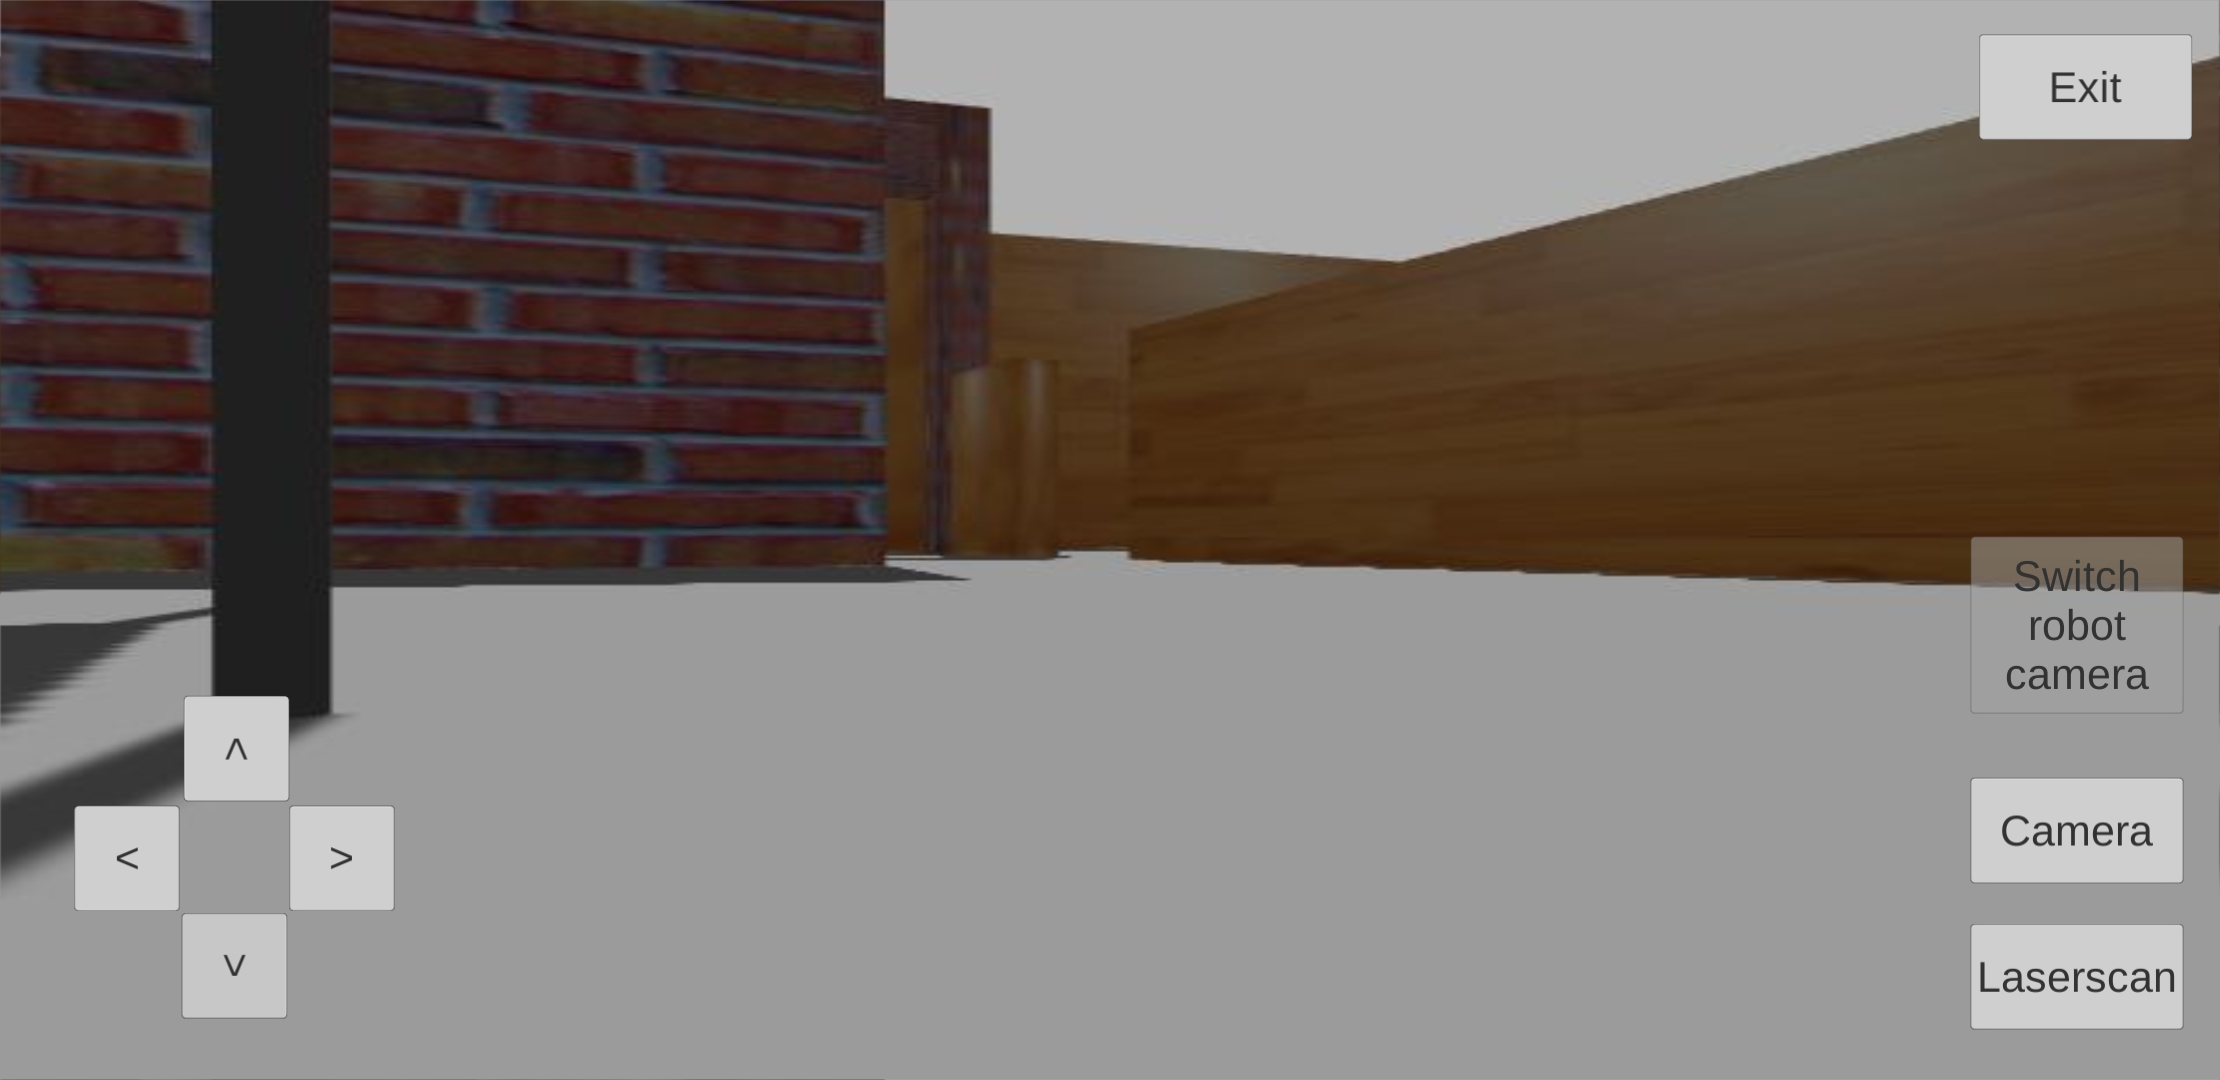
\includegraphics[height=10cm,width=10cm,keepaspectratio=true]{a2}
		\caption{Mobilna aplikacija - mapa, robot i laserski sken}
		\label{fig:a2}
	\end{center}
\end{figure}

\begin{figure}[!htbp]
	\begin{center}
		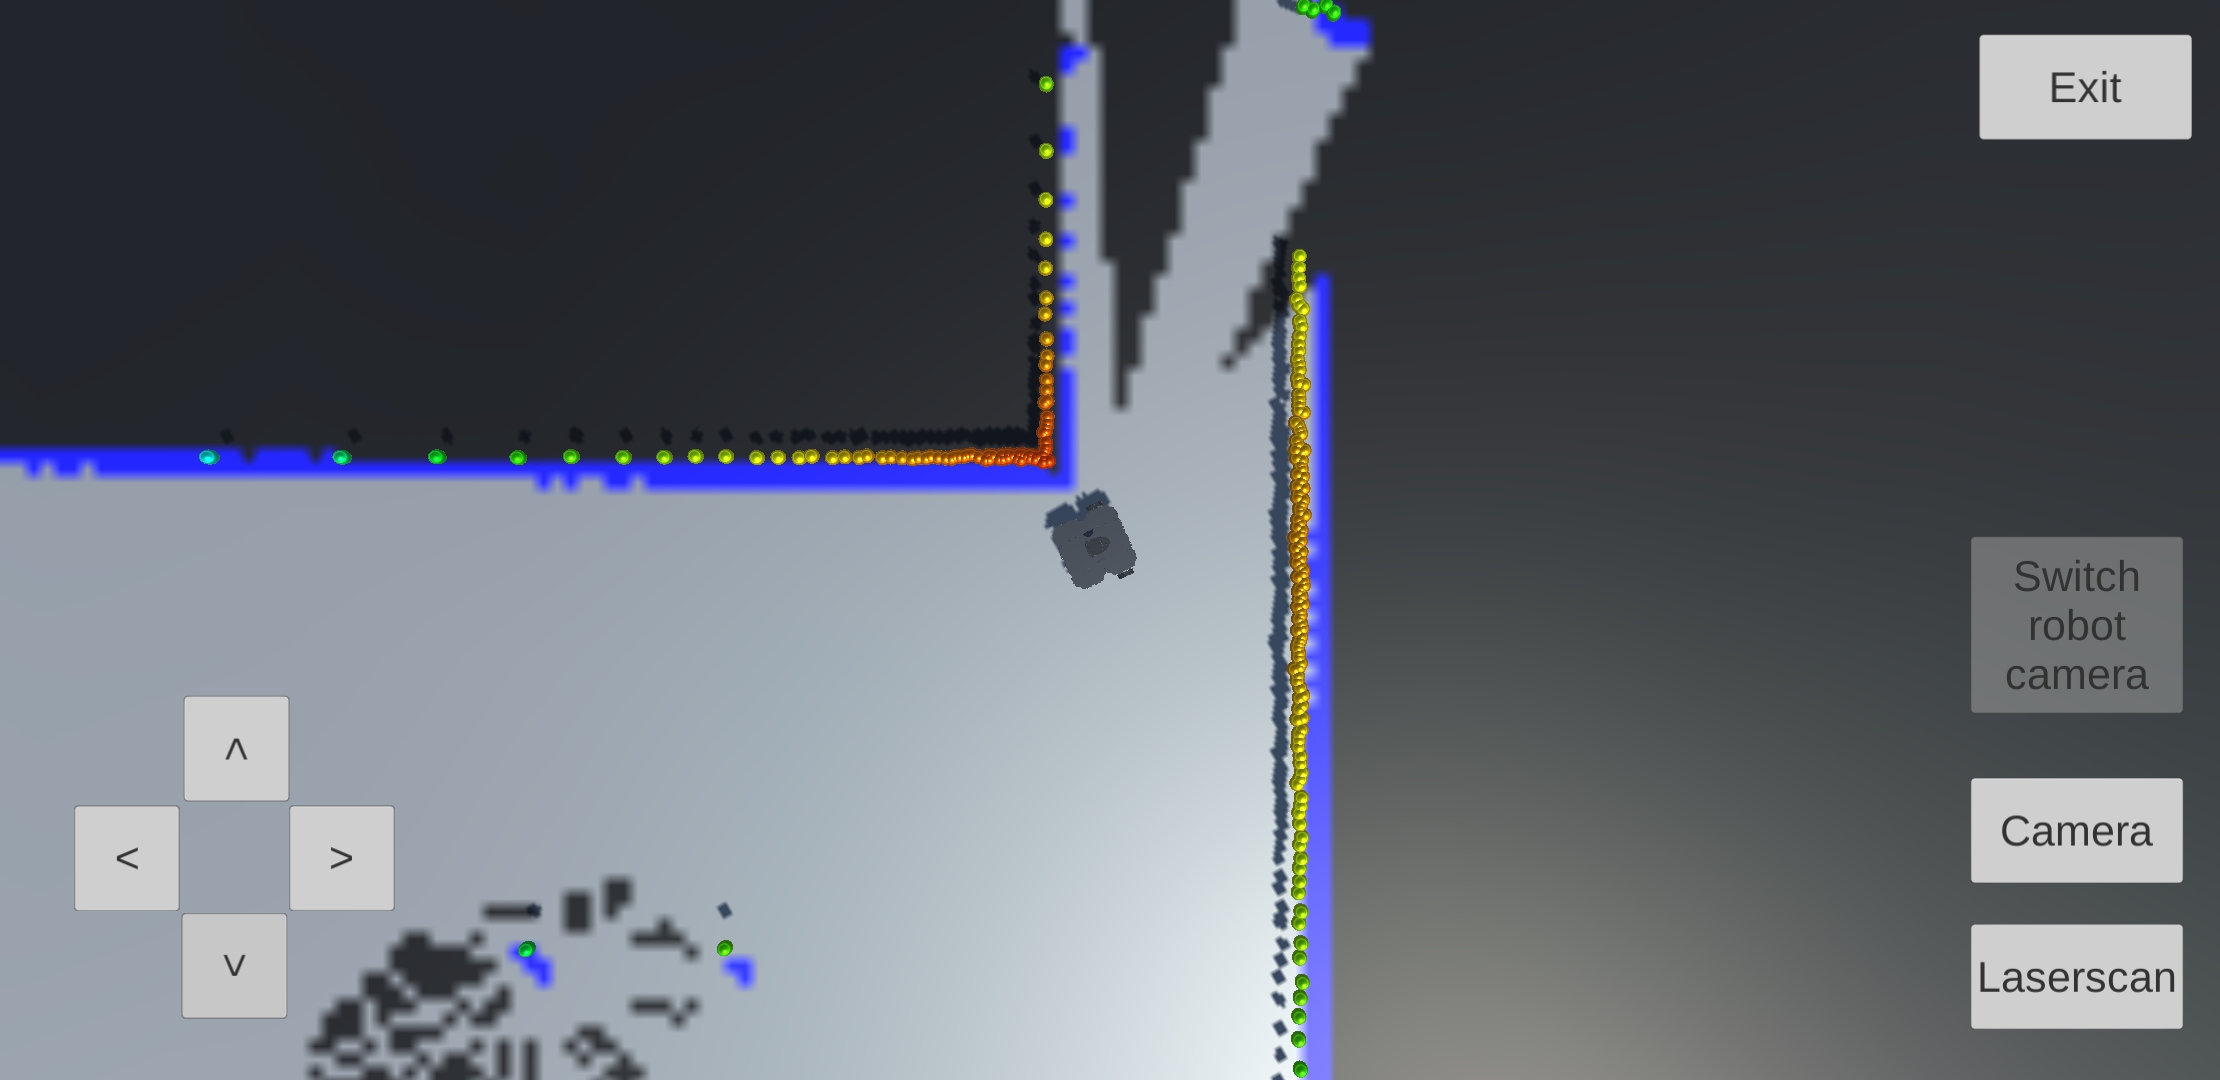
\includegraphics[height=10cm,width=10cm,keepaspectratio=true]{a3}
		\caption{Mobilna aplikacija - pogled iz kamere}
		\label{fig:a3}
	\end{center}
\end{figure}
\newpage

Na slici \ref{fig:a1} prikazana je ista scena samo u okomitom radu mobilnog ure�aja, gdje se vidi kako elementi su�elja dr�e omjer i prilago�avaju se ekranu. Potrebno je napomenuti i da se nije mijenjalo ni�ta na su�elju pri adaptaciji desktop i mobilne aplikacije ve� je to zna�ajka Unity-ja koji skalira i adaptira su�elje temeljem veli�ine ekrana, uz pretpostavku da su postavke dobro namje�tene od strane osobe koja je razvijala frontend u Unity-ju.

\begin{figure}[!htbp]
	\begin{center}
		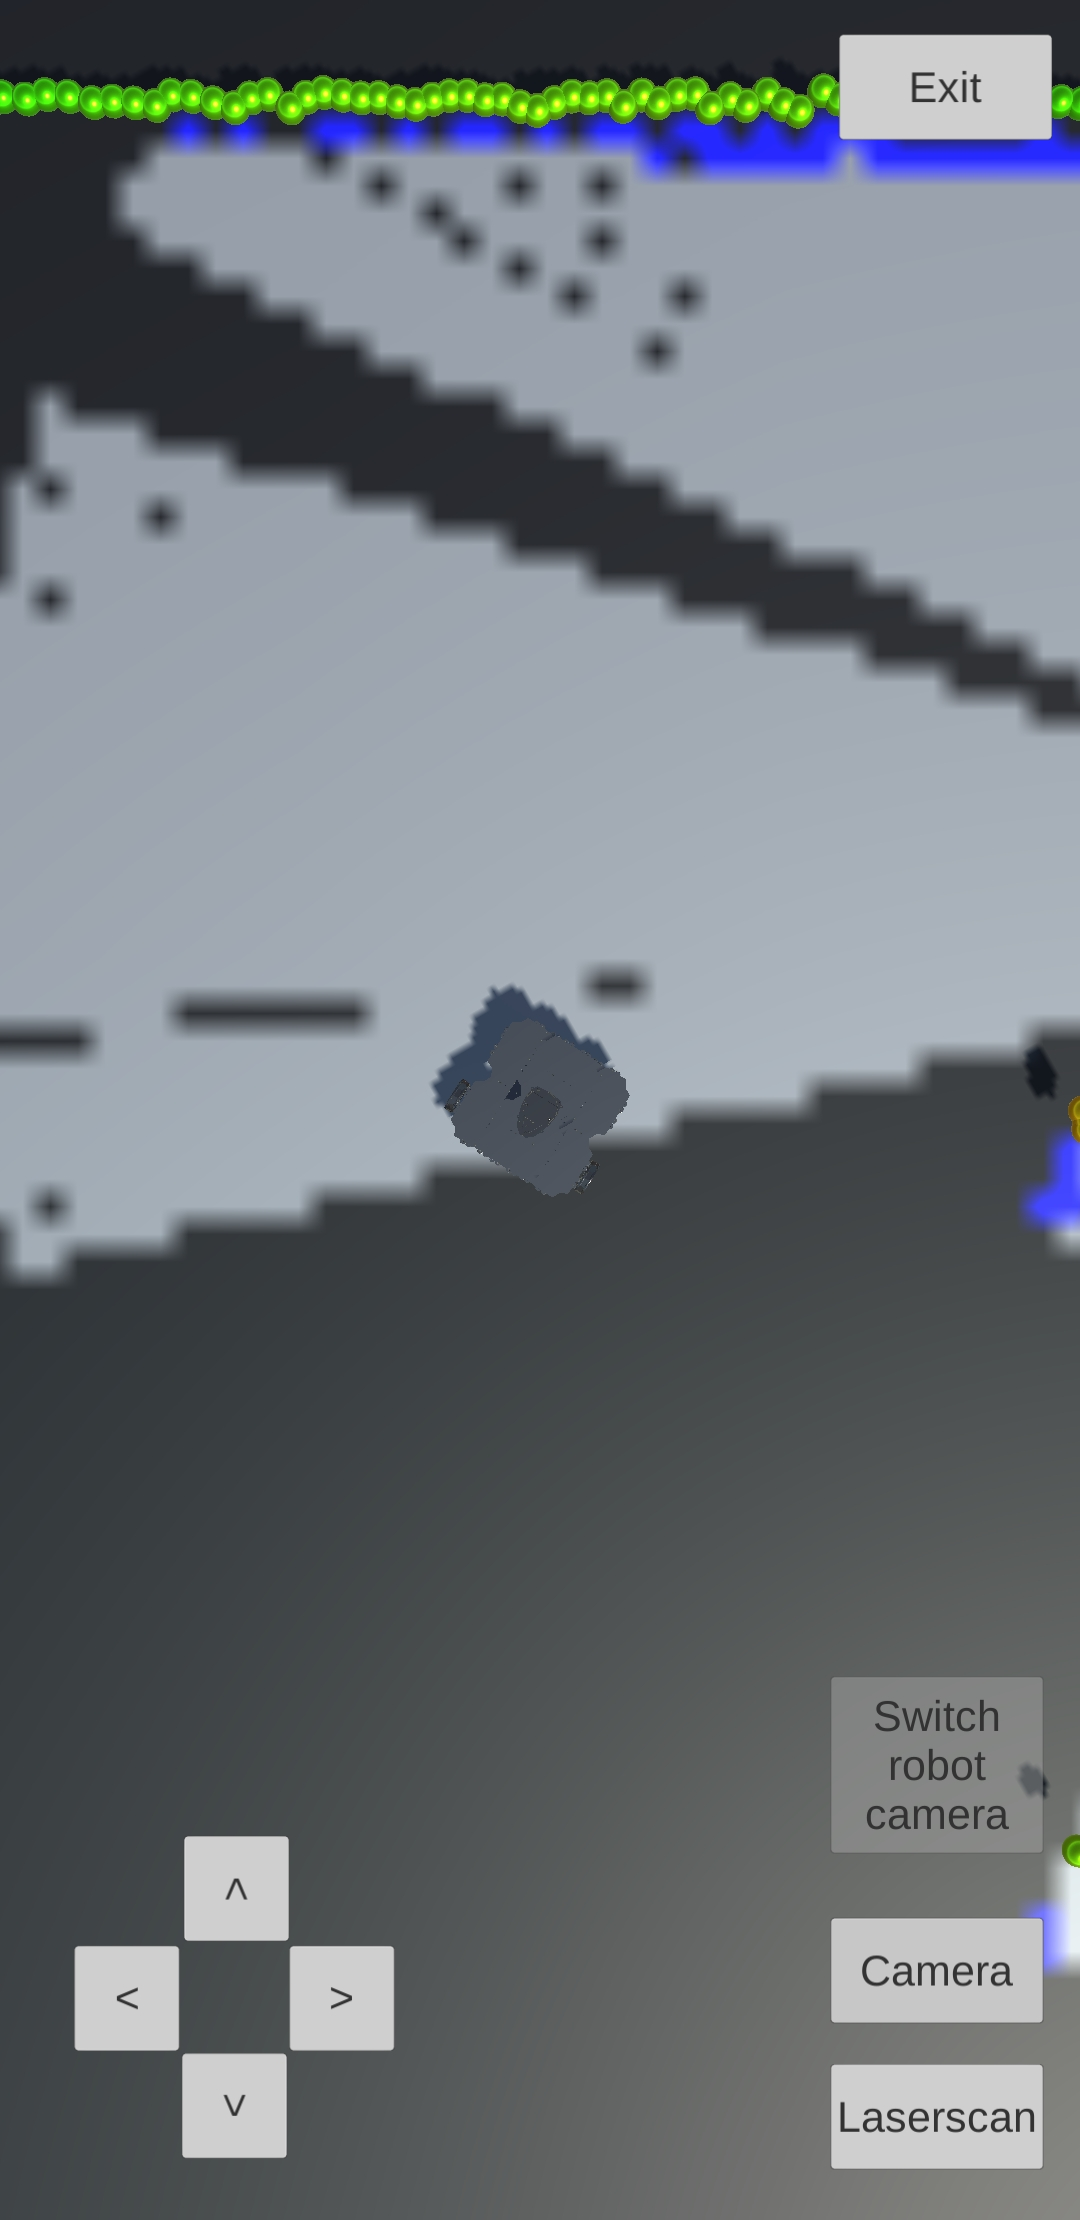
\includegraphics[height=10cm,width=10cm,keepaspectratio=true]{a1}
		\caption{Mobilna aplikacija - okomita orijentacija ure�aja}
		\label{fig:a1}
	\end{center}
\end{figure}
\clearpage

\section{Vi�e robotski prikaz}

\qquad Na sljede�oj slici, \ref{fig:linuxmulti}, prikazan je pogled s kamere jednog od dvaju robota u simulaciji. Zna�ajka prikaza kamera s oba robota radi isto na svim platformama.

\begin{figure}[!htbp]
	\begin{center}
		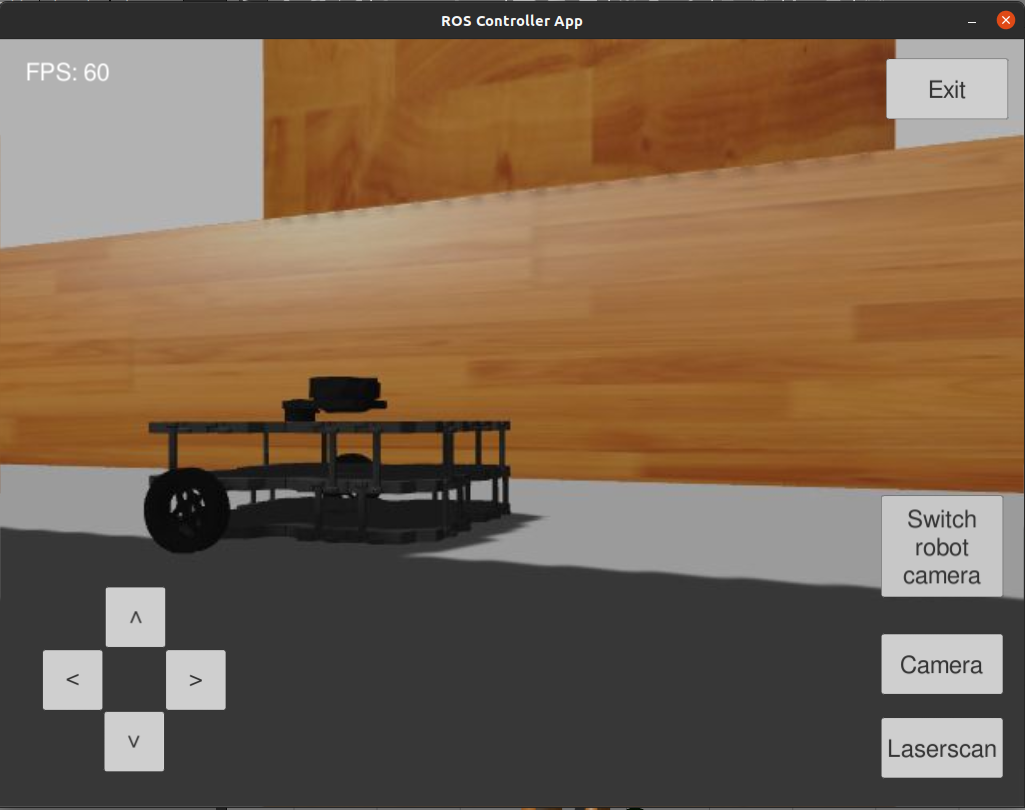
\includegraphics[height=10cm,width=10cm,keepaspectratio=true]{linuxMulti}
		\caption{Standalone aplikacija - simulacija s dva robota}
		\label{fig:linuxmulti}
	\end{center}
\end{figure}
\clearpage

\section{Problemi i pote�ko�e}

\qquad Tokom cijelog razvijanja sustava bilo je vi�e problema i pote�ko�a, od raznih inkompatibilnosti pa do ne funkcioniranja odre�enih elemenata, ali najbitnija bi bila dva problema u krajnjem rezultatu: performanse i pozicioniranje mape u Unity-ju.

Jedan od ostalih problema bio bi Unity Editor u Linux operacijskom sustavu. Unato� tome �to kroz godine podr�ka za Linux verziju Unity-ja je postala dobra te napravljena je stabilna verzija, te�ko je ne primjetiti poneke manjkavosti. Jedna od tih je slu�aj da u procesu implementiranja rje�enja, projekt se u Linux-u vi�e nije mogao pokrenuti, dok isti projekt u Windows-u je radio bez gre�aka.

\subsection{Performanse}

\qquad Kako se ve� napomenulo, performanse u Windows operacijskom sustavu su najlo�ije, dok su u ostala dva operacijska sustava solidne, no nisu savr�ene. Analiza broja a�uriranja slike u sekundi (FPS-ova - Frames Per Second), upu�uje da nije problem u tome (tablica \ref{tab:fpscompare}). Mogu�i problem bi bio u tome kako pojedina aplikacija procesira dobivene podatke zbog pretpla�ivanja na ROS teme koje stalno �alju nove poruke, no procesiranje tih poruka vr�i ROS\# i njegove skripte.

\begin{table}[!htbp]
	\scriptsize
	\renewcommand{\arraystretch}{1.2}
	\caption{FPS usporedba}
	\centering
	\begin{tabular}{|c|c|c|}
		\hline
		Android & Windows & Linux Ubuntu (prijenosno ra�unalo)
		\\ [0.5ex]
		\hline \hline
		10 - 100 & konstantno oko 99 & 100 - 1000 (integrirani ekran), manje od 100 uz vanjski monitor\\ [0.5ex]
		\hline
	\end{tabular}
	\label{tab:fpscompare}
\end{table}


\subsection{Pozicioniranje mape u Unity-ju}

\qquad Pozicioniranje mape u Unity-ju podrazumijeva na koji se na�in slika mape nacrta na \emph{Plane} objekt. Problem ovdje je taj �to se je relativno ograni�eno zbog na�ina �itanja \emph{nav\_msgs/OccupancyGrid} podataka i slijedno tome crtanju teksture gdje je vrlo te�ko napraviti precizan pomak.

Mapa se generira sukladno SLAM gmapping-u pa je ona ve�inom to�na. No kad se pozicija mape poremeti, daljnjim skeniranjem (�etanjem) prostora ona se ve�inom vrati u normalnijim okvirima (ilustracija \ref{fig:mappingsteps}). Tako�er, testiranjem se utvrdilo da je pozicija robota to�na u Unity prostoru.

\begin{figure}
	\centering	
	\subfloat[]{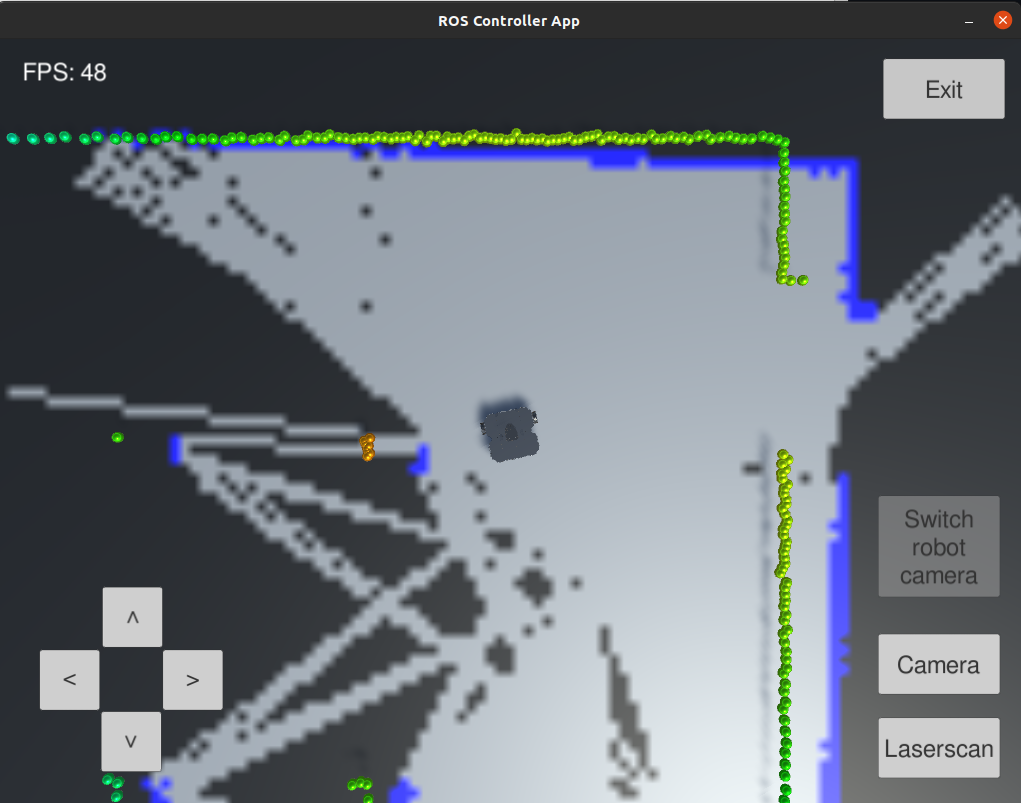
\includegraphics[width=\dimexpr(\textwidth-15pt+3pt*2)/3\relax]{map1}}\vspace{1cm}
	\subfloat[]{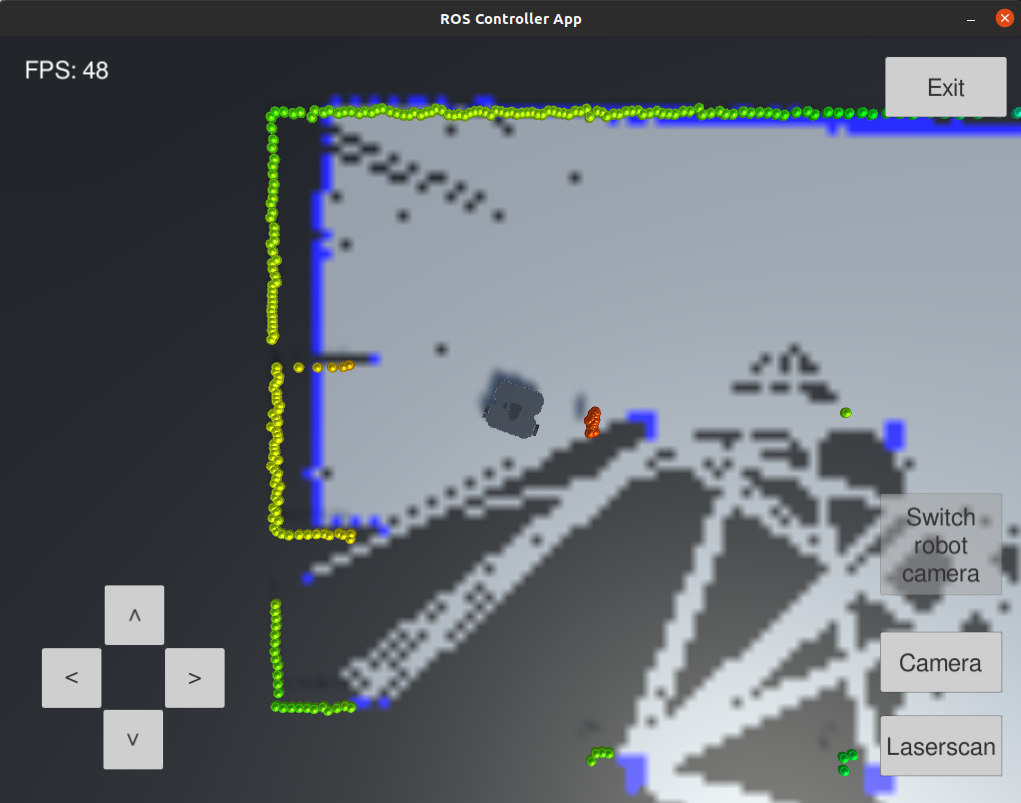
\includegraphics[width=\dimexpr(\textwidth-15pt+3pt*2)/3\relax]{map2}}\vspace{1cm}
	\subfloat[]{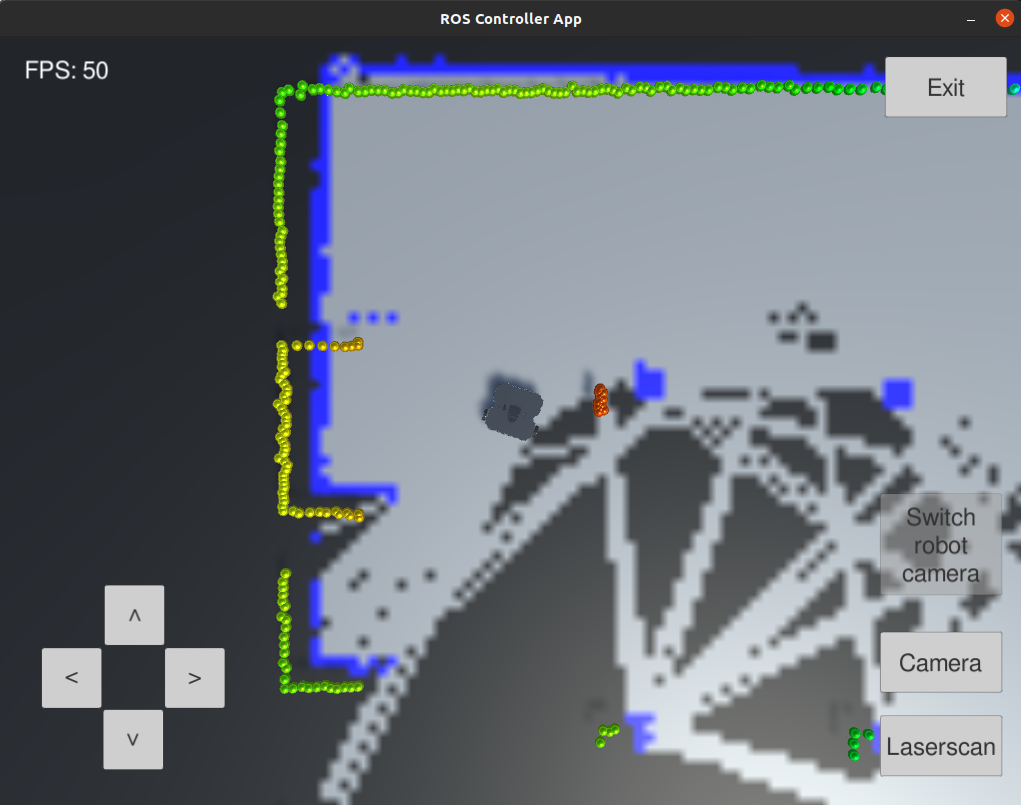
\includegraphics[width=\dimexpr(\textwidth-15pt+3pt*2)/3\relax]{map3}}\\
	\subfloat[]{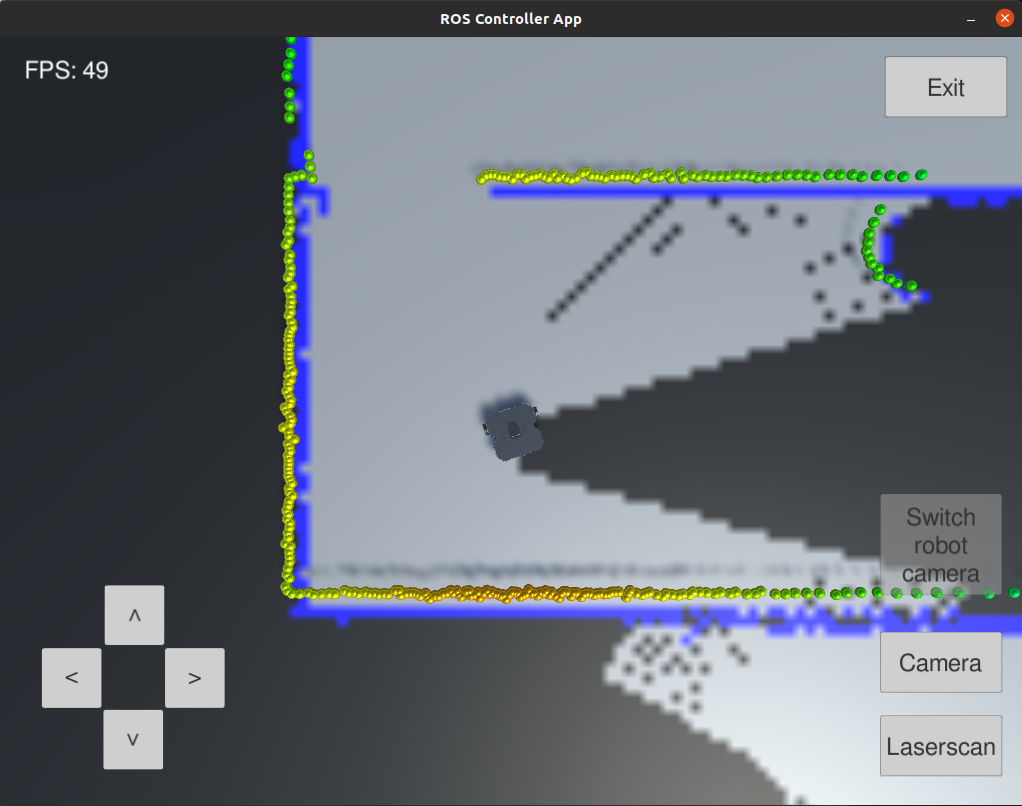
\includegraphics[width=\dimexpr(\textwidth-15pt+3pt*2)/3\relax]{map4}}\vspace{1cm}
	\subfloat[]{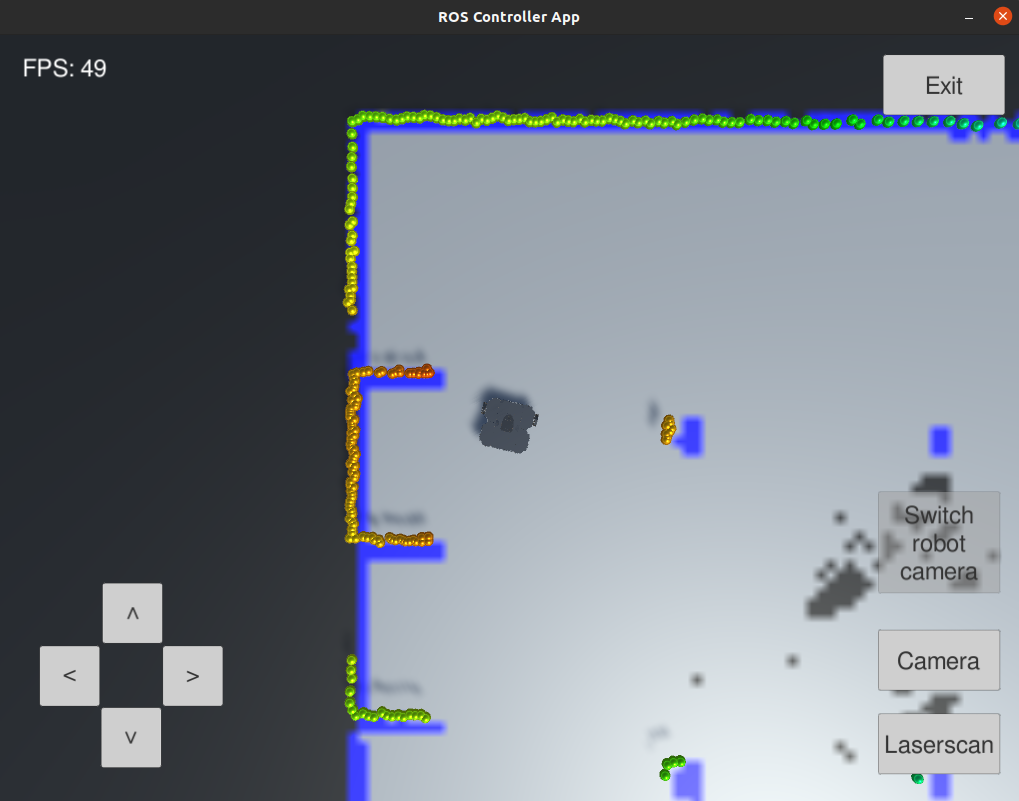
\includegraphics[width=\dimexpr(\textwidth-15pt+3pt*2)/3\relax]{map5}}
	\caption{Koraci mapiranja}
	\label{fig:mappingsteps}
\end{figure}

 
% !TeX encoding = windows-1250
\chapter{Zaklju�ak}

\qquad U ovom se radu razvila aplikacija za upravljanje robotom i mapiranje prostora koriste�i \emph{SLAM gmapping} za 2D mapu te \emph{Octomap mapping} za 3D mapu. Paralelno s upravljanjem robota generira se 2D mapa prostora, nalik tlocrtu zgrade. Tako�er, omogu�eno je generiranje sfera iz podataka laserskog skena, kao i prikaz iz prvog lica kamere robota. U slu�aju vi�e robota u simulaciji, mogu�a je promjena perspektive s jedne kamere robota na kameru drugog robota. Napravljeno je i generiranje 3D mape prostora u stvarnom vremenu koje se odra�uje u zasebnoj sceni.

Aplikacija je ra�ena isklju�ivo koriste�i Turtlebot 3 - Waffle simuliranog robota. Za adaptaciju na drugu vrstu robota dovoljno je u�itati novi URDF model te eventualno izmijeniti ROS teme u \emph{RosConnectoru} u slu�aju da se razlikuju.

Aplikacija je izgra�ena i testirana na tri platforme: Windows, Linux Ubuntu i Android. Mogu�e je uz minimalne promjene aplikaciju izgraditi i za Mac OS. Performanse aplikacija nisu savr�ene kao �to je navedeno u zadnjem poglavlju rada, gdje iste ovise o fazi rada i kori�tenom hardveru. U fazi 1 gdje je kori�tena \emph{Waffle Pi} ina�ica Turtlebota aplikacija za Windows je drasti�no lo�ija od ostalih iako je sve prakti�ki isti kod. Naime, u fazi 2 je kori�tena \emph{Waffle} ina�ica Turtlebot-a s kamerom koja omogu�ava 3D percepciju prostora gdje je fluidnost slike kamere drasti�no pala. Me�utim, scena koja generira 3D mapu sa�uvala je logi�nost izme�u kori�tenog hardvera i performansa aplikacije gdje su ra�unalne verzije odr�ale normalan i konstantan broj a�uriranja slike u sekundi (FPS), a mobilna se verzija uvelike usporila.

ROS\# se pokazao kao alat s vrlo velikim potencijalom za izradu konkretnijih aplikacija, kao i za edukacijske svrhe te za entuzijaste koji rade s Unity razvojnim okru�enjem.

Zaklju�no, glavni cilj ovog rada - spajanje robota na Unity i implementiranje multiplatformske aplikacije, dodatno podi�e mogu�nosti ROSa i Unityja koji zajedno mogu dovesti do vrlo zanimljivih i korisnih rezultata. 
% !TeX encoding = windows-1250
%I) rucno upisati svaku referencu redoslijedom kojim se prvi puta pozivaju u tekstu
%\begin{thebibliography}{99}
%
%\bibitem{html} .....opis reference .........
%
%\bibitem{php} .......opis reference ........
%
%\bibitem{ajax}  .........opis reference..........
%
%\end{thebibliography}


%II) bolji nacin: pomocu programa JabRef opisati svoje reference i pohraniti u datoteku ``Literatura.bib''. U tekstu samo pozivati zeljene reference, a lista se sama formira.

\bibliographystyle{tex_aux/IEEEtranHR}  % ``unsrt'', ``IEEEtran'', ``ieeetr''
% argument is your BibTeX string definitions and bibliography database(s)

\bibliography{Literatura}
  % ovo je ime Bibtex datoteke koju korisnik kreira


%:::::::::: ukljucenje popisa kratica u tekst ::::::::
% Blok linija koda ispod ovoga generira ukljucenje popisa kratica u tekstu. Za uporabu, vidjeti Upute.
% Nije obavezno. Ako se ne zeli koristiti, onda ovaj blok staviti u komentar pomocu znaka %
%\printglossary[type=\acronymtype]
%\pagestyle{plain}
%\begin{glossary}{Longest string}%
%	%%%%%%%%%%%%%%%%%%%%%%%%%%%%%%%%%%%%%%%%%%%%%%%%%%%%%%%%%%%%%%%%%%%%%%%%%%%%%%%%%%%%%%%%%%%%%%%%%
%% ovo je jednostavniji (ali neautomatski) primjer definiranja liste akronima, a student neka to zamijeni svojim kraticama i doda sve koje zeli
%% ako se ne zeli deklarirati popis kratica, onda ga staviti pod komentar u glavnoj datoteci
%
%   \item[{\bf HTML}]	Hypertext Markup Language
%   \item[{\bf AJAX}]	Asynchronous JavaScript and XML

%%%%%%%%%%%%%%%%%%%%%%%%%%%%%%%%%%%%%%%%%%%%%%%%%%%%%%%%%%%%%%%%%%%%%%%%%%%%%%%%%%%%%%%%%%

%%%%%%%%%%%%%%%%%%%%%%%%%%%%%%%%%%%%%%%%%%%%%%%%%%%%%%%%%%%%%%%%%%%%%%%%%%%%%%%%%%%%%%%%%%
% Sofisticiraniji nacin definiranja i uporabe kratica je preko sljede�e sintakse

 \addcontentsline{toc}{chapter}{Pojmovnik}
% primjeri definicije kratica
% ove pojmove zamijenite nekim svojima i po tom predlosku nadogradite listu po potrebi
\newacronym{nfc}{NFC}{Near Field Communication}
\newacronym{wlan}{WLAN}{Wireless Local Area Network} 
\newacronym{gsm}{GSM}{Global System for Mobile (Communications)}


%::::::::: UPORABA KRATICA U TEKSTU :::::::::::::::::
% u tekstu jednostavno na mjestu gdje �elite koristiti odre�enu kraticu, upotrijebite naredbu 
%  \gls{id_kratice}, kao npr. \gls{nfc}
% i u tekstu �e vam automatski biti uba�ena kratica kako je definirana u drugoj zagradi u gornjim definicijama, a ako je u uporabi prvi puta, tada �e prvo biti naveden puni naziv, kako je definiran u tre�oj zagradi, a potom kratica. Za sve ostale slu�ajeve uporabe, bit �e navedena samo kratica.

%:::::::::::::::::::::::::::::::::::::::::::::::::::::
%  podsjetnik nekoliko mogu�ih oblika sintakse
% op�a uporaba: \gls{nfc} % mo�e i za rje�nik i za kratice. Prvi poziv daje dugi i kratki naziv (redoslijedom koji je specificiran u preambuli pomocu \setacronymstyle, a od drugi puta nadalje samo kraticu.
% ako �elite nametnuti ba� neki oblik kori�tenja kratice, imate sljede�e naredbe
%\acrshort{nfc} \\  % samo akronim
%\acrfull{nfc} \\   % akronim i puni naziv
%\acrlong{nfc} \\   % samo puni naziv

%::::::::::::::::::::::::::::::::::::::::::::::::::::
% Kako se generira Pojmovnik u tekstu:
%1. pokrenite LaTeX kompilaciju 1x
%2. u Command Promptu odite radnu mapu gdje su vam datoteke diplomskog rada i utipkajte
%	makeindex -s myDoc.ist -o myDoc.gls   myDoc.glo
%	
%	gdje myDoc zamijenite imenom svoje glavne .tex datoteke (JMBAG_Ime_Prezime.tex)
%3. pokrenite LaTeX kompilaciju jos jednom

%::::::::::::::::::::::::::::::::::::::::::::::::::::
%\end{glossary}


%:::::::::::: blok za definiranje Sazetka/Abstracta rada 
\begin{abstract}
	% !TeX encoding = windows-1250
\vspace{5pt}

%:::::::::::::::::::::::::::::::::::::::::::::::::::::
%:::::::::::: HRVATSKI :::::::::::::::::::::::::::::::
\noindent
Cilj ovog rada bio je napraviti funkcionalnu aplikaciju za upravljanje robotom i mapiranje prostora. Mapiranje se vr�i paralelno uz upravljanje robotom. Izra�uje se 2D mapa koja se prikazuje ispod robota. Omogu�en je prikaz podataka s laserskog skena u obliku sfera i prikaz iz prvog lica kamere robota. U svrhu istra�ivanja implementirano je da se u slu�aju dvaju robota u simulaciji mo�e mjenjati pogled kamere s jednog robota na drugi. Aplikacija je funkcionalna na tri platforme: Windows, Linux i Android. Performanse aplikacije su dobre, osim na Windows operacijskom sustavu.
%:::::::::::::::::::::::::::::::::::::::::::::::::::::

\vspace{5pt}
%
\noindent \textbf{\textit{Klju�ne rije�i} --- ROS, Unity, ROS\#, upravljanje robotom, mapiranje} 

%:::::::::::: KRAJ HRVATSKOG DIJELA :::::::::::::::::::


%::::::::::::::::::::::::::::::::::::::::::::::::::::::
%:::::::::::: ENGLESKI ::::::::::::::::::::::::::::::::

%\vspace{-10pt}
\section*{Abstract}
\vspace{-10pt}
The objective of this thesis was to make a functional application for robot control and mapping. Mapping is done in parallel with the robot control. A 2D map is being made which is shown under the robot. Laser scan data is displayed in a form of spheres and a first person view from the robot camera was also enabled. For research purposes in the case of two robots in the same simulation, a feature was implemented for switching the camera view from one robot to another. The application is functional on three platforms: Windows, Linux and Android. Performance of the applications is good, except on the Windows operating system.
%:::::::::::::::::::::::::::::::::::::::::::::::::::::::

\vspace{5pt}
%
\noindent \textbf{\textit{Keywords} --- ROS, Unity, ROS\#, robot control, mapping}

%::::::::::::::::::::::::::::::::::::::::::::::::::::::
%:::::::::::: KRAJ ENGLESKOG DIJELA :::::::::::::::::::

	  % sazetak rada i kljucne rijeci na HR i EN
\end{abstract}


%:::::::::::: PRILOZI (neobavezno) ::::::::::::::::::::
% ispod \appendix zaglavlja pomocu \include dodati poglavlja s prilozima
% ukoliko nemate priloga, ovaj blok linija staviti u komentar
\appendix
% !TeX encoding = windows-1250
\chapter{Konfiguracija radne okoline}
\qquad U ovom �e se poglavlju opisati postupak konfiguriranja radne okoline. Ovo je potrebno iz razloga �to ve�ina alata nije testirana na najnovijim Ubuntu i ROS verzijama pa su odre�ene adaptacije bile potrebne.

\qquad Instalaciju i konfiguraciju se mo�e podijeliti u nekoliko koraka, od kojih �e se pojasniti samo one koji su zahtjevali dodatne korake:
\begin{enumerate}
	\item Instalacija Ubuntu 20.04 OS-a.
	\item Instalacija ROS-a Noetic Ninjemys-a gdje je potrebno pratiti upute na slu�benim stranicama. Vr�i se instalacija potpunog paketa.
	\item Instalacija Unity-ja. Dobro je povremeno instalirati noviju verziju jer sadr�i korisna a�uriranja.
	\item Instalacija Visual Studio Code-a - text editor koji �e se koristiti uz Unity za programiranje skripta. Razlog odabira Visual Studio Code-a je taj �to je potrebno imati podr�ku za Unity i mogu�nost spajanja i pokretanja alata za otklanjanja pogre�ka (debugger).
	\item Instalacija .NET Core radne okoline za omogu�iti rad Unity-ja s Visual Studio Code - podr�ka za C\#. \cite{netcoreinstall}
	\item Visual Studio Code konfiguracija za Unity. \cite{vscodeconfig} 
	\item Instalacija \textit{Mono} radne okoline. \cite{monoinstall} Preporu�ljivo je nakon ovog koraka pokrenuti i naredbu \textit{sudo apt install mono-complete} da bi se instalirali eventualni segmenti koji fale.
	\item Instalacija Turtlebot 3 paketa za ROS 1. \cite{turtlebotinstall}
\end{enumerate}

\section{Dodatni koraci}
\qquad Ovdje �e biti navedeni i eventualno poja�njeni dodatni koraci. Neki od tih su jednostavna instalacija dodatnog paketa, a neki promjene da bi odre�ena stvar mogla proraditi.

\qquad Kada je neki alat ili knji�nicu u ROS-u potrebno instalirati iz izvornog koda, to se u osnovi radi na sljede�i na�in (eventualni alati imaju specificirana potrebna dodatna pode�avanja):
\begin{enumerate}
	\item Preuzimanje i spremanje mape s datotekama izvornog koda u ROS radni folder (workspace - \textit{~/catkin\_ws/src/}) - ova mapa je proizvoljna ali ROS standard je \textit{catkin\_ws} u \textit{home} direktoriju Linux Ubuntu OS-a.
	\item U korijenskom \textit{catkin\_ws} direktoriju pokre�e se naredba \textit{catkin\_make} koja izgradi sav kod u njemu. Tada se pojave dvije nove mape - \textit{build} i \textit{devel}. Nakon toga treba pozvati izgenerirani \textit{setup.bash} sljede�om naredbom koja omogu�ava kori�tenje novo izgra�enih paketa:
	
\textit{source /home/user/catkin\_ws/deve/setup.bash} ili \textit{source /opt/ros/noetic/setup.bash}
\end{enumerate}

\begin{itemize}
	\item Za omogu�iti mapiranje robotske okoline potrebno je dodatni instalirati \textit{slam} pakete za mapiranje. Instalacija se vr�i iz izvornog koda kojeg je mogu�e dohvatiti s git repozitorija paketa \cite{percgit} gdje se nalazi i drugih paketa za robotsku percepciju. 
	\item Osnovna spona koja omogu�uje slanje podataka izme�u ROS-a i Unity-ja je \textit{RosBridge} paket kojeg ina�e dohva�amo naredbom \textit{sudo apt-get install ros-noetic-rosbridge-server}. Istoga koristi ROS\#. ROS Noetic-u instalacija ovog paketa na klasi�an na�in ne radi, ali vi�e o tome u sljede�em odlomku.
	\item Za kori�tenje �eljenog robota u Unity, prvi korak je unijeti njegov model. Koristi se URDF (Universal Robotic Description Format - univerzalni robotski opisni format). URDF je pisan u XML formatu i koristi se za opisati sve elemente opisanog robota. 
\end{itemize}

\subsection{Uvoz URDF modela u Unity}
\qquad Za uvoz URDF modela potrebno je pokrenuti odre�enu \textit{launch} datoteku koja se nalazi u ros-sharp (datote�no prihvatljiv naziv za ROS\#) paketu. Datoteka se nalazi u \textit{ros-sharp/ROS/file-server/launch}, odnosno \textit{catkin\_ws/src/file-server/launch} direktoriju koja se pokre�e \textit{roslaunch publish\_description\_turtlebot.launch} no prije samog pokretanja potrebno ju je urediti iz razloga �to je to samo primjer za Turtlebot 2 robot, koji ima druga�ije specifikacije od Turtlebot 3 robota.

\qquad \textit{Launch} datoteke su tako�er pisane u XML formatu i one slu�e za pokretanje vi�e �vorova odjednom. U datoteci se mo�e podesiti i dodatne parametre za pokretanje odre�enih �vorova. \textit{Roslaunch} je kori�ten za pokretanje tih datoteka i to se mo�e u�initi pozivanjem paketa i specifi�ne \textit{launch} datoteke ili direktno pozivanjem \textit{launch} datoteke definiranjem njezine datote�ne putanje:

\qquad - \textit{roslaunch ime\_paketa launch\_datoteka}

\qquad - \textit{roslaunch ../catkin\_ws/src/paket/launch/launch\_datoteka}

\qquad Osim ure�ivanja robotskih vrijednosti, potrebno je i urediti i argument \textit{urdf\_file} na na�in da se iz \textit{xacro.py} izbaci \textit{.py} te doda flag \textit{--inorder}. To se mora iz razloga �to su sve prija�nje verzije ROS-a bile na Python 2, ali je ROS Noetic na Python-u 3. (slika~\ref{fig:urdfimportlaunch})

\begin{figure}[!htbp]
	\begin{center}
		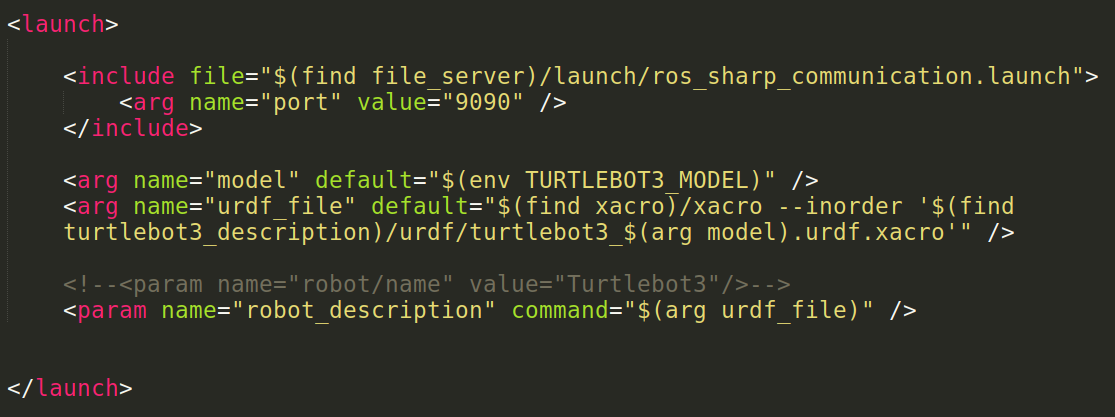
\includegraphics[height=6cm,width=12cm,keepaspectratio=true]{URDFImportLaunch}
		\caption{Launch datoteka za URDF uvoz}
		\label{fig:urdfimportlaunch}
	\end{center}
\end{figure}

\qquad Jo� jedna promjena koja je potrebna a povezana je s verzijama Python-a je za uspje�no pokretanje \textit{RosBridge} poslu�itelja. Naime, ako se izvr�i instalacija standardnom \textit{apt install} naredbom, RosBridge ne�e raditi jer se kose vrste varijabla (\textit{str} i \textit{byte}) koje su druga�ije definirane u svakoj verziji Python-a, pa je iz tog razloga potrebno instalirati cijeli RosBridge iz izvornog koda \cite{rosbridgegit} uz namje�tenu to�nu verziju Python-a (2).

\qquad Nakon ovih koraka mo�e se pokrenuti Unity i u izborniku odabrati \textit{RosBridgeClient - Transfer URDF from ROS} gdje se otvara prozor�i� (slika~\ref{fig:urdfimport}) u kojemu je potrebno izmijeniti IP adresu gdje �e se prona�i RosBridge poslu�itelj. Ostale vrijednosti bi trebale biti dobre po zadanim vrijednostima. Prije spajanja, potrebno je pokrenuti TurtleBot simulaciju i gore navedenu \textit{launch} skriptu. Dovr�etkom ovog koraka, u Unity projekt se sprema URDF model kojega se mo�e prikazati i koristiti u scenama.

\begin{figure}[!htbp]
	\begin{center}
		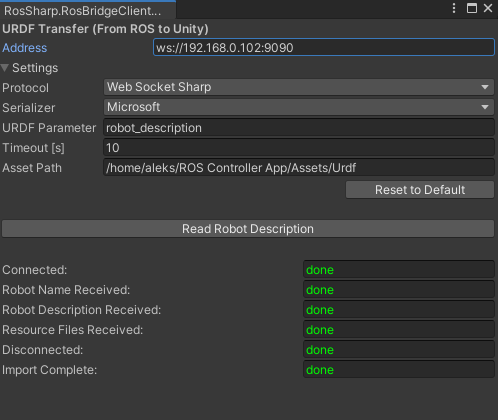
\includegraphics[height=6cm,width=12cm,keepaspectratio=true]{URDFImport}
		\caption{URDF uvoz}
		\label{fig:urdfimport}
	\end{center}
\end{figure}


\qquad Za kori�tenje simuliranog okru�enja koristi ste \textit{Gazebo} softver, no iz razloga limitirane kompatibilnosti umjesto zadnjeg Gazebo 11, u slu�aju da simulacija ne radi, potrebno je instalirati Gazebo 9 pakete:

\qquad \textit{sudo apt install gazebo9-common}

\qquad \textit{sudo apt-get install libgazebo9-*}

\qquad \textit{sudo apt install ros-noetic-gazebo-ros-pkgs}


\subsection{Dodatno}

\qquad Dodatne informacije o konfiguriranju dostupne su na slu�benom ros-sharp repozitoriju u sekciji wiki stranica. \cite{rossharprepo}

\qquad Tako�er, u slu�benom repozitoriju nalaze se Unity testne scene s kojima se mo�e testirati osnovne funkcionalnosti.

% !TeX encoding = windows-1250

\section{Glavna launch datoteka}

\begin{lstlisting}
<launch>
	<include file="$(find rosbridge_server)/launch/rosbridge_websocket.launch">
	<param name="port" value="9090"/>
	</include>
	<include file="$(find turtlebot3_slam)/launch/turtlebot3_slam.launch">
	<param name="slam_methods" value="gmapping"/>
	</include>
	
	<!-- One robot -->
	<include file="$(find turtlebot3_gazebo)/launch/turtlebot3_house.launch">
	</include> 
	
	<!-- Multiple robots 	
	<include file="$(find turtlebot3_gazebo)/launch/multi_turtlebot3.launch">
	</include> -->	
	
	<node name="file_server" pkg="file_server" type="file_server" />
	
	<node name="joy_to_twist" pkg="gazebo_simulation_scene" type="joy_to_twist.py"/>
	
	<node name="rqt_graph" pkg="rqt_graph" type="rqt_graph" />
	
	<node name="laserScanCorrector" pkg="gazebo_simulation_scene" type="laserScanCorrector.py" />
</launch>
\end{lstlisting} 
% !TeX encoding = windows-1250

\section{Ostalo}

\qquad Ostale relevantne launch datoteke, Unity projekt i drugo biti �e prilo�eni kao zasebne datoteke.
  



\end{document}
